\documentclass[conf]{new-aiaa}
%\documentclass[journal]{new-aiaa} for journal papers
\usepackage{preamble}

\begin{document}


\begin{titlepage} % Suppresses displaying the page number on the title page and the subsequent page counts as page 1
	\newcommand{\HRule}{\rule{\linewidth}{0.5mm}} % Defines a new command for horizontal lines, change thickness here
	
	\center % Centre everything on the page
	
	%------------------------------------------------
	%	Headings
	%------------------------------------------------
	
	\textsc{\LARGE University of Illinois at Urbana-Champaign\\ \vspace{10pt}Department of Aerospace Engineering}\\[1.5cm] % Main heading such as the name of your university/college
	
	\textsc{\Large Team Toucans}\\[0.5cm] % Major heading such as course name
	
	\textsc{\large SAM Mk. I}\\[0.5cm] % Minor heading such as course title
	
	%------------------------------------------------
	%	Title
	%------------------------------------------------
	
	\HRule\\[0.4cm]
	
	{\huge\bfseries Final Design Report}\\[0.4cm] % Title of your document
	
	\HRule\\[1.5cm]
	
	%------------------------------------------------
	%	Author(s)
	%------------------------------------------------
	
	\begin{minipage}{0.4\textwidth}
		\begin{flushleft}
			\large
			\textit{Authors}\\
			Joshua \textsc{Clements}\\
			Chris \textsc{Endres}\\
			Jack \textsc{Johnson}\\
		\end{flushleft}
	\end{minipage}
	~
	\begin{minipage}{0.4\textwidth}
		\begin{flushright}
			\large
			\textit{}\\
			Mateusz \textsc{Korzen}\\
			Kacper \textsc{Piechnik}\\
			Nicole \textsc{Zaworski}
		\end{flushright}
	\end{minipage}
	
	%------------------------------------------------
	%	Pictures
	%------------------------------------------------
	
        \begin{figure}[H]
            \centering
            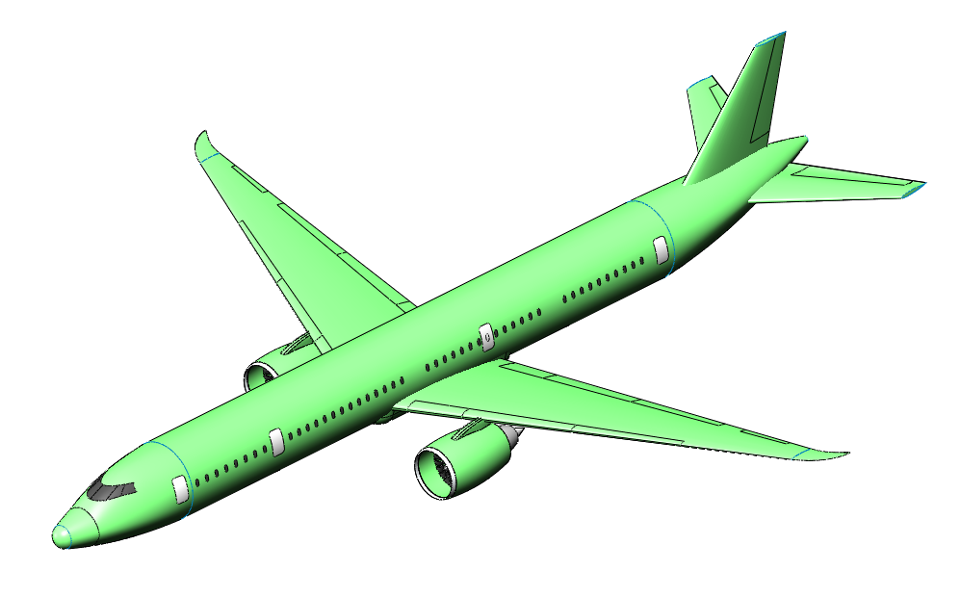
\includegraphics[width=0.98\linewidth]{Photos/Toucan SAM Mk. I Isometric FDR.jpeg}
            \label{figISO}
        \end{figure}
	%Isometric_Aircraft__2-12-20_-Transparent Background.png
	%------------------------------------------------
	%	Date
	%------------------------------------------------
	
	\vfill\vfill\vfill % Position the date 3/4 down the remaining page
	
	{\large April 30\textsuperscript{th}, 2020} % Date, change the \today to a set date if you want to be precise
	
	%------------------------------------------------
	%	Logo
	%------------------------------------------------
	
	\vfill\vfill
	\begin{minipage}{\linewidth}
		\begin{flushright}
	        
\includegraphics[scale=0.5]{Photos/Illinois-Logo-Full-Color-RGB.png}\\[1cm]
		\end{flushright}
	\end{minipage}
	 
	%----------------------------------------------------------------------------------------
	
	\vfill % Push the date up 1/4 of the remaining page
	
\end{titlepage}




% \begin{titlepage}
%     \begin{center}
%         \vspace*{1cm}
%         {\LARGE \textbf{Design Readiness Report} \\
%         \vspace{0.5cm}
%         \textbf{Team Toucan}} \\
%         \vspace{0.5cm}
%         {\normalsize
%         \textbf{by} \\
%         \vspace{0.5cm}
%         \textbf{Joshua Clements, Chris Endres, Jack Johnson,\\ Mateusz Korzen, Kacper Piechnik and Nicole Zaworski} \\
%         \vspace{0.5cm}
%         {\large\textbf{AE443 Senior Design II}}\\
%         \vspace{0.5cm}
%         \textbf{February 13th, 2020}} \\
%         \vspace{0.5cm}
%         {\large University of Illinois at Urbana-Champaign \\ Department of Aerospace Engineering \\ 104 S Wright St, Urbana, IL 61801} \\
%         \vspace{2.0cm}
        
%         \begin{figure}[H]
%             \centering
%             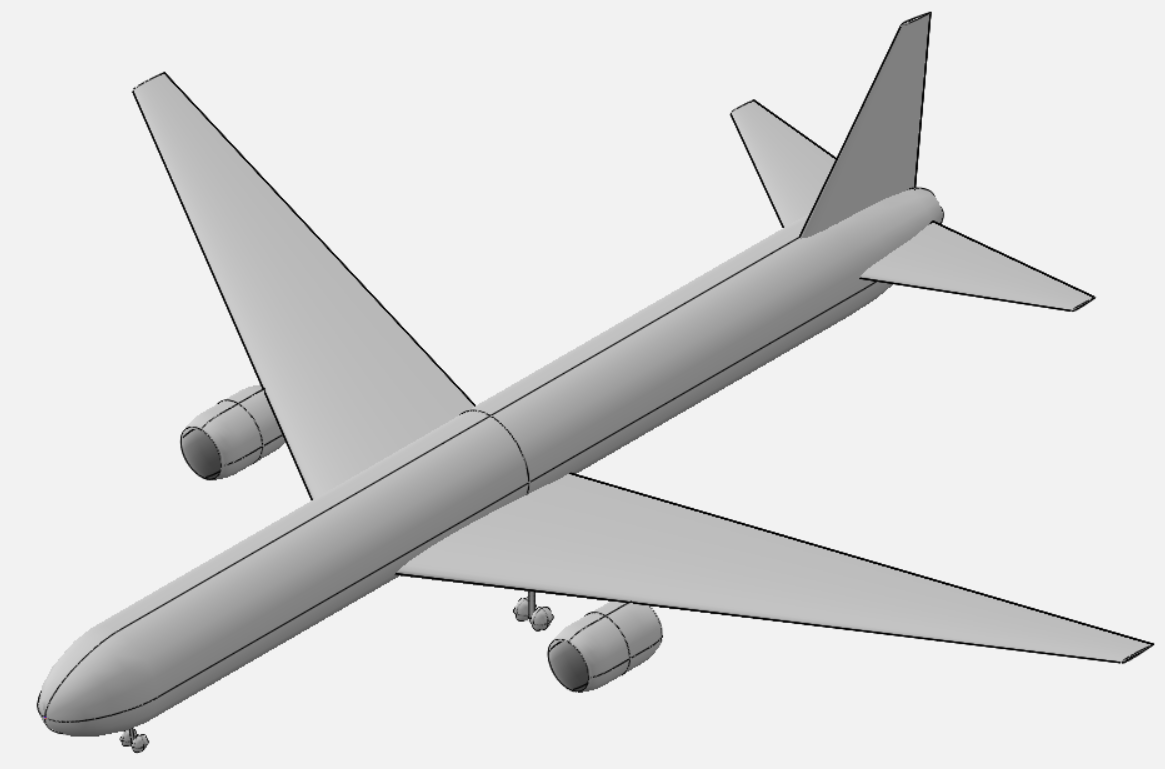
\includegraphics[width=0.70\linewidth]{Photos/Isometric_Aircraft (2-12-20).png}
%             \label{figISO}
%         \end{figure}
%         \vspace{2.0cm}
%         %{\Large
%         %$\bullet$\\
%         %\vspace{2.5cm}
%         %$\bullet$\\
%         %\vspace{2.5cm}
%         %$\bullet$\\
%         %\vspace{1.75cm}}
%         {\normalsize
%         \textbf{Faculty Advisor:} Dr. Jason Merret}\\
%         %\textcolor{red}{Include A/C drawings or team logo}
%     \end{center}
% \end{titlepage}

\newpage

\pagenumbering{roman}
\begin{figure}[!h]
    \centering
    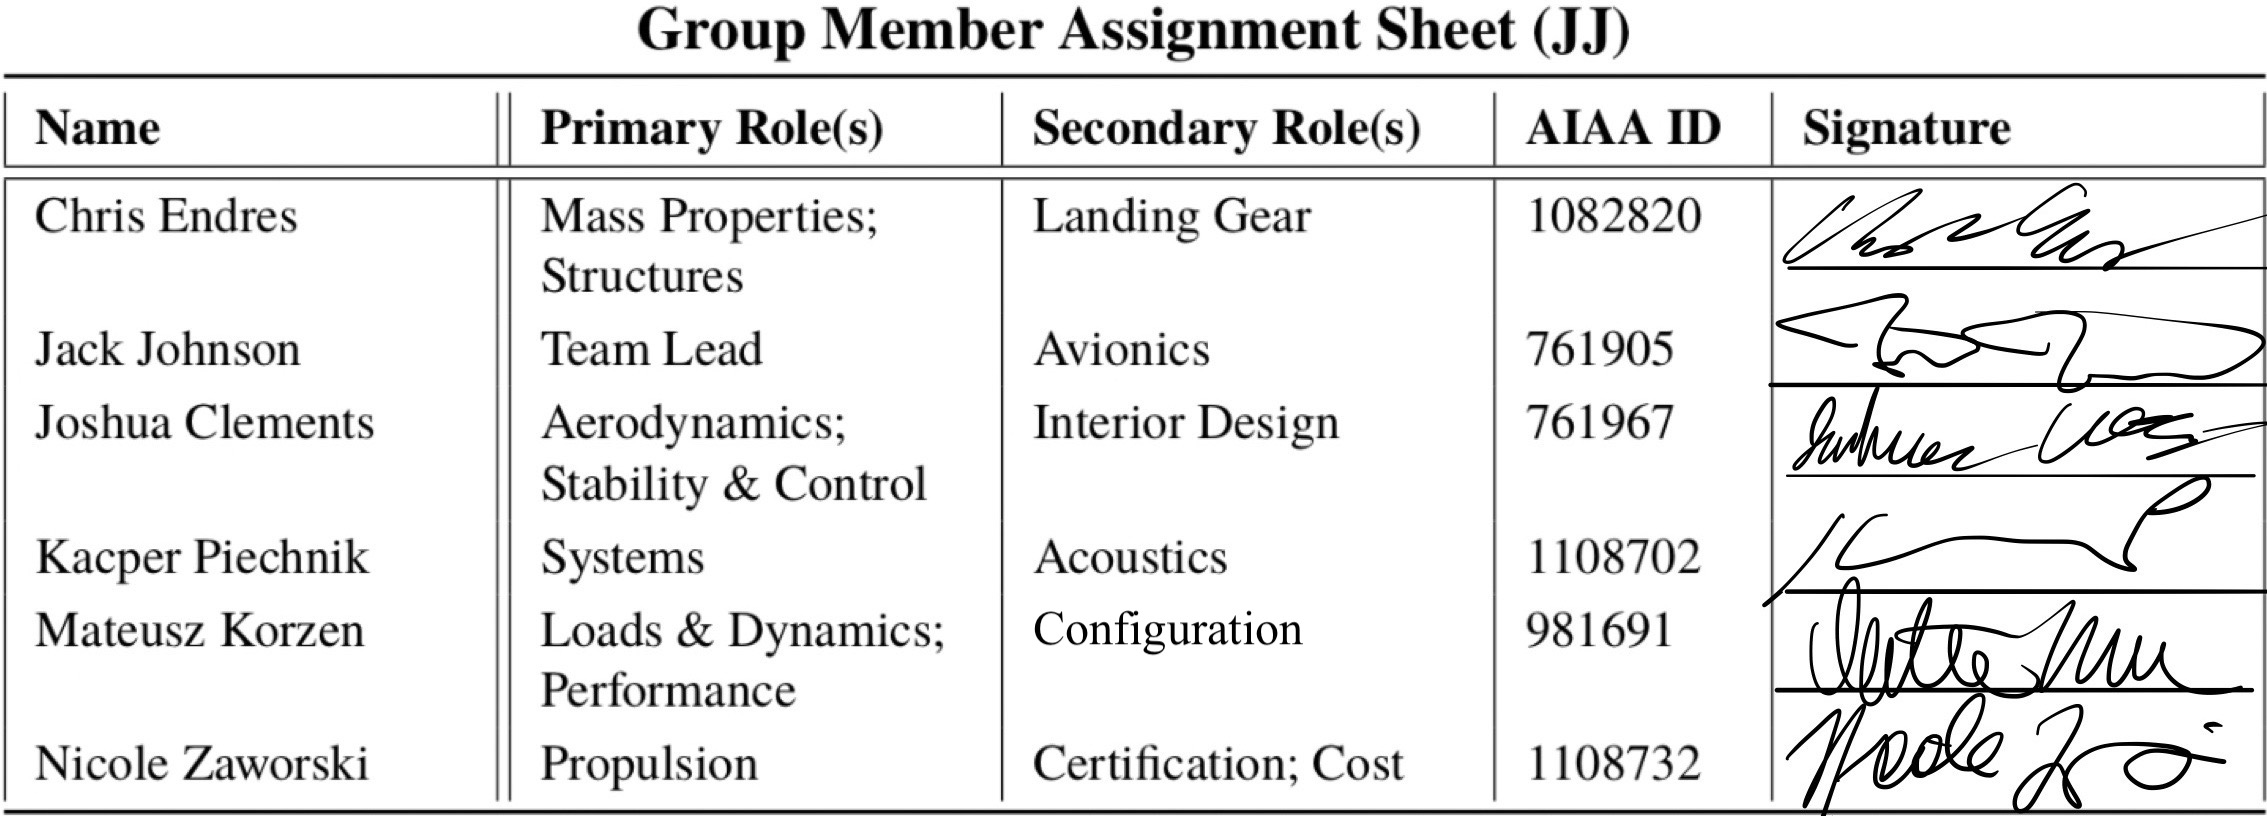
\includegraphics[width=\linewidth]{Photos/signatures.JPG}
    \label{fig:my_label}
\end{figure}

\begin{center}
\large{ \textbf{Team Toucan}}
\end{center}

\begin{figure}[!h]
    \centering
    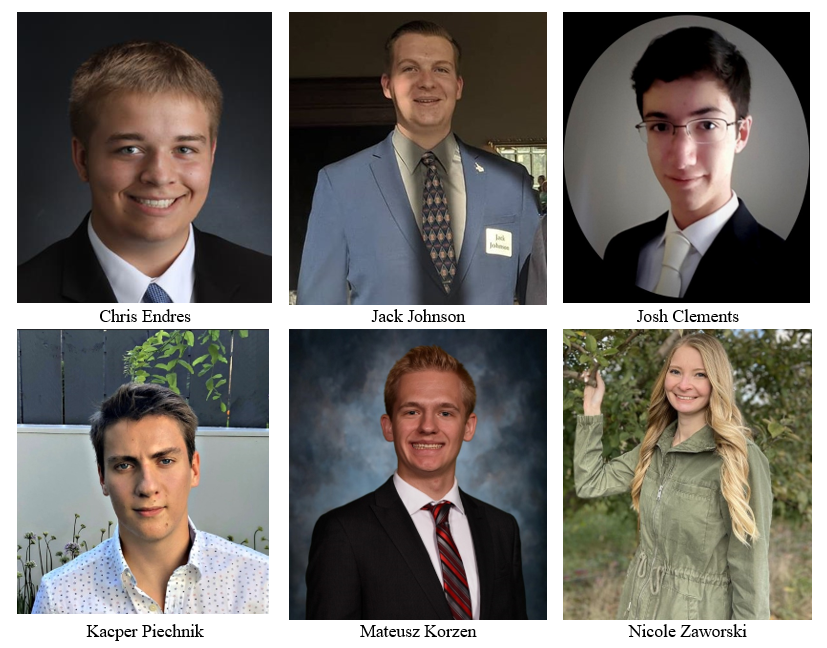
\includegraphics[width=\linewidth]{Photos/Toucan Headshots.png}
    \label{fig:my_label}
\end{figure}



% \section*{Group Member Assignment Sheet (JJ)}
% \begin{center}
%     \begin{tabular}{ |p{3cm}||p{3cm}|p{3cm}|p{1.5cm}|p{3cm}| }\toprule
%         %  \multicolumn{5}{c}{Team Roster} \\\midrule
%          \textbf{Name} & \textbf{Primary Role(s)} & \textbf{Secondary Role(s)} & \textbf{AIAA ID} & \textbf{Signature} \\\hline \hline
%          Chris Endres & Mass Properties; \newline Structures & Landing Gear & 1082820 & \\
%          Jack Johnson & Team Lead & Avionics & 761905 & \\ 
%          Joshua Clements & Aerodynamics; \newline Stability \& Control & Interior Design & 761967 & \\ 
%          Kacper Piechnik & Systems & Acoustics & 1108702 & \\ 
%          Mateusz Korzen & Loads \& Dynamics; \newline Performance & Configuration & 981691 & \\ 
%          Nicole Zaworski & Propulsion & Certification; Cost & 1108732 & \\\bottomrule 
%     \end{tabular}
% \end{center}

\newpage
\tableofcontents
\renewcommand{\thesection}{\arabic{section}}

\section{List of Figures}
\makeatletter
\@starttoc{lof}% Print List of Figures
\makeatother

\section{List of Tables}
\makeatletter
\@starttoc{lot}% Print List of Tables
\makeatother

\newpage


\section{Nomenclature}
\hspace{-0.5in}\textbf{Abbreviations and Acronyms}
{\renewcommand\arraystretch{1.0}
\noindent\begin{longtable*}{@{}l @{\quad=\quad} l@{}}
    A/C & Aircraft \\
    AIAA & American Institute of Aeronautics and Astronautics \\
    ALT & Approach, Landing, and Taxi \\
    AR & Aspect Ratio \\
    % AEI & All Engines Inoperative \\
    APU & Auxiliary Power Unit \\
    % BFL & Balanced Field Length \\
    % BL & Boundary Layer \\
    % BPR & Turbofan engine bypass ratio \\
    % CAD & Computer Aided Design \\
    % CAS & Calibrated Airspeed \\
    % CER & Cost Estimated Relationship \\
    CFD & Computational Fluid Dynamics \\
    CFR & Code of Federal Regulations \\
    CFRP & Carbon Fiber Reinforced Polymer \\
    CG & Center of Gravity \\
    ConOps & Concept of Operations \\
    % CTOL & Conventional Take-off and Landing \\
    % DARPA & Defense Advanced Research Projects Agency \\
    % DoD & Department of Defense \\
    % EAS & Equivalent Airspeed \\
    ECU & Engine Control Unit \\
    ENCU & Environmental Control Unit \\ 
    EDP & Engine Driven Pump \\
    FAA & Federal Aviation Administration \\
    FADEC & Full Authority Digital Engine Control \\
    FWB & Fly-By-Wire \\
    FEA & Finite Element Analysis \\
    FAR & Federal Aviation Regulations (certification specs) \\
    % FAR & Federal Acquisition Regulations \\
    FBW & Fly By Wire \\
    FCS & Flight Control System \\
    % FOD & Foreign Object Damage \\
    FLXXX & Flight Level of XXX Hundreds of Feet \\
    FQIS & Fuel Quantity Indicating System \\
    % GA & General Aviation \\
    GPS & Global Positioning System \\
    IAS & Integrated Avionics System \\
    ICAO & International Civil Aviation Organization \\
    IDG & Integrated Drive Generator \\
    IFR & Instrument Flight Rules \\
    ILS & Instrument Landing System \\
    % IPPD & Integrated Product and Process Development \\
    % IR & Infrared \\
    % IOS & International Standards Organization \\
    % JATO & Jet-Assisted Take off \\
    % KISS & KEEP IT SIMPLE, STUPID! (Ed Heinemmann) \\
    % LCC & Life-cycle cost \\
    % LOX & Liquid Oxygen \\
    % L\&P & Leakage and Protuberances \\
    LPV & Localizer Performance with Vertical Guidance \\
    % MDO & Multidisciplinary Design Optimization \\
    Mk. & Mark \\
    % MSL & Mean Sea Level \\
    in & inch \\
    ISA & International Standard Atmosphere \\
    KCAS & Knots Calibrated Airspeed \\
    KEAS & Knots Equivalent Airspeed \\
    kts & Knots \\
    lb & Pound \\
    LFL & Landing Field Length \\
    MAC & Mean Aerodynamic Chord \\
    MLS & Microwave Landing System \\
    MTOW & Maximum Take-off Weight \\
    MZFW & Maximum Zero Fuel Weight \\
    % NASA & National Aeronautics and Space Administration \\
    % NAV & Navigation \\
    NM & Nautical Mile  \\ % \cite{nautical}
    % NS & Navier-Stokes (high-end CFD) \\
    NVIS & Near Vertical Incidence Skywave \\
    % OEM & Original Equipment Manufacturer \\
    OEI & One Engine Inoperative \\
    % OML & Outer Mold Lines \\
    % RCS & Radar Cross Section \\
    % RCS & Reaction Control System \\
    % RFI & Request for Information \\
    RFP & Request for Proposals \\
    % RFQ & Request for Quotations \\
    RNP & Required Navigation Performance \\
    % RPM & Revolutions per Minute \\
    RVSM & Reduced Vertical Separation Minimum \\
    S\&C & Stability and Control \\
    SFC & Specific Fuel Consumption \\
    % SL & Sea Level \\
    % SOP & Standard Operating Procedure \\
    % STOL & Short Take-off and Landing \\
    % TAS & True Airspeed \\
    TO & Take Off \\
    TOFL & Takeoff Field Length \\
    % TVC & Thrust Vector Control \\
    % UAV & Unmanned Aerial Vehicle \\
    USD & US Dollar \\
    VFR & Visual Flight Rules \\
    VNAV & Vertical Navigation \\
    VOR & Very High Frequency (VHF) Omni-Directional Range \\
    % VTOL & Vertical Take-off and Landing \\
    WAAS & Wide Area Augmentation System \\
    WUTTO & Warm-up, Taxi, and Takeoff \\
    ZFW & Zero Fuel Weight\\
\end{longtable*}}

\hspace{-0.5in}\textbf{Coefficients}
{\renewcommand\arraystretch{1.0}
\noindent\begin{longtable*}{@{}l @{\quad=\quad} l@{}}
    $\alpha$ & Angle of Attack \\
    b & Wing Span \\
    c & Chord length \\
    $C_D$ & Wing Drag Coefficient \\
    $C_d$ & Airfoil Drag Coefficient \\
    $C_{D,i}$ & Induced Drag Coefficient \\ %will this later apply to the whole plane?
    $C_{D,0}$ & Zero-Lift Drag / Parasitic Drag \\
    $C_{D,W_{NL}}$ & Wave Drag due to shock induced on non-lift generating surfaces \\
    $C_{D,W_{L}}$ & Wave Drag due to shock induced on lift generating surfaces \\
    $C_{D_{EXCR}}$ & Drag due to surface roughness \\
    $C_{D,trim}$ & Drag due to Trim surfaces \\
    $C_f$ & Skin Friction Coefficient \\
    $C_L$ & Wing Lift Coefficient \\ %will this later apply to the whole plane?
    $C_l$ & Airfoil Lift Coefficient \\
    e & Oswald Efficiency Factor \\
    % FF & Form Factor Term for parasitic drag calculation \\
    % g & Gravity (Earth = 9.81 $\frac{m}{s^2}$ \\
    $h_p$ & Pressure Altitude \\
    % Isp & Specific Impulse \\
    % K & Drag due to lift factor \\
    $\lambda$ & Wing Taper Ratio ($C_{tip} / C_{root}$) \\
    % L/D & Lift to Drag ratio \\
    % LE & Leading Edge \\
    M & Mach Number \\
    % m & Total aircraft mass \\
    % $M_{cr}$ & Critical Mach number \\
    % $M_{dd}$ & Drag Divergent Mach number \\
    % n & Load factor \\
    % Q & Interference factor for parasitic drag calculation \\
    % $q_{\infty}$ & Dynamic pressure \\
    % Re & Reynolds Number \\
    % S & LE Suction \\
    % $\mathcal{S}$ & Wing Area \\
    T/W & Thrust-to-weight ratio \\
    % t & Airfoil thickness \\
    t/c & Airfoil thickness-to-chord length ratio \\
    TE & Trailing Edge \\
    % TO & Take-off \\
    % $V_{NE}$ & Never Exceed Speed \\
    % $V_{1}$ & TO Decision Speed \\
    % $V_2$ & TO Safety Speed \\
    $W_e$ & Empty Weight\\
    $W_f$ & Fuel weight \\
    % $W_o$ & TO Gross Weight \\
    % W/S & Wing Loading \\
\end{longtable*}}
% \hspace{-0.5in}\textbf{Greek Symbols}
% {\renewcommand\arraystretch{1.0}
% \noindent\begin{longtable*}{@{}l @{\quad=\quad} l@{}}
%     $\alpha$ & Angle of Attack \\
%     % $\beta$ & Prandtl-Glauert Compressibility correction \\
%     % $\delta_f$ & Flap Deflection \\
%     % $\Lambda$ & Sweep Angle \\
%     % $\epsilon$ & Unit Strain \\
%     % $\gamma$ & Shearing Strain \\
%     % $\Gamma$ & Wing Dihedral Angle \\
%     % $\eta$ & Efficiency \\
%     $\lambda$ & Wing Taper Ratio ($C_{tip} / C_{root}$) \\
%     % $\mu$ & Viscosity \\
%     % $\rho$ & Air Density \\
%     % $\sigma$ & Air density ratio ($=\rho/\rho_o$) \\
%     % $\tau$ & Unit Shear Stress \\
% \end{longtable*}}



\newpage
\doublespacing


\section{Executive Summary (\textit{JJ})}
\label{section: Exec Summary}
%\begin{singlespace}

The following design report represents the basis for a new aircraft developed by Team Toucan at the University of Illinois at Urbana-Champaign in response to AIAA's Request for Proposal \cite{RFP} (RFP) addressing the industry need for a high capacity, short to medium haul widebody capable of mitigating the increased traffic and congestion found at many modern airports.  While the design aircraft will be capable of carrying up to 400 passengers up to 3,500 NM, it has been engineered to bridge the gap between low capacity, short range regional jets and high capacity, long range twin jets currently on the market.  This report validates the possibility of addressing the prescribed requirements in a commercial aircraft.

 Prominent driving design points of the SAM Mark I include takeoff and landing distances under 9,000 ft, maximum range of 3,500 NM, capacity of 400 passengers and their respective luggage, 10 person crew (two pilots, eight flight attendants), adherence to FAA 14 CFR Part 25 regulations and fundamental desire to maximize customer value through minimizing fuel consumption as well as other operating costs.  The proposed aircraft will be service-ready by 2029 and has been designed as a twin engine, twin aisle widebody with a traditional tail.  Most notably, the entire wing including its sub-structure will be designed and manufactured utilizing modern composites to minimize structural weight while not sacrificing performance or longevity.  Other value-added design points include leading and trailing edge high lift devices, visual flight rule (VFR) and instrument flight rule (IFR) flight with autopilot, and de-icing capability for flight in less than ideal weather conditions.

\begin{table}[!h] 
    \centering
    \caption{At a Glance: Toucan Aviation's SAM Mark I}
    \begin{tabular}{ |c|c|c|c|c|c| }\toprule
    \textbf{Capacity} & \textbf{MTOW} & \textbf{Range} & \textbf{TOFL} & \textbf{LFL} & \textbf{Cruise Speed} \\\hline 
    400 Passengers & 457,390 [lb] & 3,500 [NM] & 9,000 [ft] & 9,000 [ft] & Mach 0.775  \\\hline \hline
    \textbf{SFC} & \textbf{TO Thrust} & \textbf{Wing Span} & \textbf{AR} & \textbf{MAC} & \textbf{Service Ceiling}  \\\hline 
    0.545 [lbm/lbf/hr] & 231,080 [lb] & 184 ft 5 in & 8.5 [$\sim$] & 25 ft 6 in & FL480  \\\hline \hline
    \textbf{Wing Loading} & \textbf{Thrust/Weight} & \textbf{Wing} & \textbf{Fuselage} & \textbf{Cost/Flight Hour} & \textbf{Flyaway Cost/1000}  \\\hline 
    114.35 [lb/ft$^2$] & 0.505 [$\sim$] & Composite & Metallic & \$82,379 [USD] & \$181,204,000 [USD] \\ \bottomrule

    \end{tabular}\label{tab:ataglance}
\end{table}

Important aircraft parameters are illustrated in Table \ref{tab:ataglance}.  These values have evolved from the original seed and fundamental based design after an in-depth analysis of their aerodynamic and performance implications.  Leading edge slats and trailing edge,  Fowler-type flaps are designed and integrated into the wing structure to efficiently generate lift under critical conditions such as take-off and landing.  Presentation of this final design follows a detailed finite element analysis (FEA) and computational fluid dynamics (CFD) analysis of the complete aircraft's aerodynamic surfaces and structure in order to ensure flight worthiness and is accompanied a thorough approximation of assembly cost, timeline, and life cycle maintenance costs.  A complete review of FAA 14 CFR Part 25 \cite{cfr} and the AIAA RFP \cite{RFP} has been completed to ensure delivery of a safe, value-driven aircraft for the AIAA 2020 undergraduate design competition.

%Considerable effort will continue to be put into meeting or exceeding applicable FAA 14 CFR Part 25 requirements for commercial aircraft, and final design will be completed by April 26, 2020 leaving adequate time for review, system integration check, FAR compliance check and submission of a safe, value-driven aircraft design by May 14th, 2020.

% \begin{table}[h!] 
%     \centering
%     \caption{Design Timeline $\&$ Team Waypoints}
%     \begin{tabular}{ |c||c| }\toprule
%     \textbf{Date} & \textbf{Task(s)} \\\hline\hline
%     3/30/2020 & Revision per FDR Comments Deadline \\\hline
%     4/6/2020 & Absolute Geometry Deadline \\ \hline
%     4/20/2020 & Computer-analysis/Derivation $\&$ Presentation Deadline \\ \hline
%     4/21/2020 & Final Design Presentation Deadline \\ \hline
%     4/26/2020 & Final Design Report Writing $\&$ Review Deadline \\ \hline
%     4/30/2020 & Final Design Submission \\ \hline
%     5/14/2020 & AIAA Submission \\\hline
%     \end{tabular}\label{deadlines}
% \end{table}

%\end{singlespace}

% \textcolor{red}{
% \begin{itemize}
%     \item Briefly discuss motivation for the aircraft, key requirements, and your design drivers. (JC \checkmark)
%     \item Briefly  summarize the proposed aircraft, including key  characteristics (e.g. general configuration, \textbf{TOGW, primary dimensions), key performance metrics, key differentiators, and a cost summary.} (JC \checkmark)
%     \item Include any requirements not met, struggling with, or have chosen to exceed. \textbf{(none?)}
%     \item Discuss the near term milestones and provide a project timeline for the semester. 
%     \item Maximum length: one page, single-spaced if necessary. (JC \checkmark)
% \end{itemize}}

%FROM DRR:
%Additionally, a component wise weight build up of corrected values for hybrid construction will supplement an in-depth stability and control analysis.  


\clearpage
\setcounter{section}{0}
\renewcommand{\thesection}{\Roman{section}}
\pagenumbering{arabic} % MODIFYING PAGINATION FROM ROMAN TO ARABIC

\section{Introduction (\textit{JJ})}
\label{section: Intro}
The SAM Mark I has been developed to solve one of aviation's biggest challenges: congested airports in urban areas prone to significant delays.  As airlines continue to embrace the hub and spoke model, it becomes ever apparent modern aviation has ignored one of the biggest necessities in the market - a high capacity plane optimized to handle shorter routes while still retaining the capability of long-haul nonstop flight between the world's major destinations. A twin engine wide body, the Sam Mark I will be capable of comfortably carrying 400 passengers in a 50/350 two-class configuration with adequate range to fly transatlantic from the Eastern seaboard to popular European destinations, as well as many other routes under 3,500 nmi.  Unlike many competitors, the SAM Mark I takes full advantage of contemporary composites and high-lift devices in order to feature a fully composite wing adjacent to traditional fuselage, resulting in a significant increase in performance and added value to the end user.  This value will only increase as populous economies across the world mature, resulting in an increased demand on commercial aviation that not only fits within but also fully utilizes the existing infrastructure. 

% \textcolor{red}{
% \begin{itemize}
%     \item Discuss motivation, design objectives (e.g design drivers, key requirements), and a summary of key design characteristics and capabilities. \checkmark (\textit{JC})
%     \item This section should identify your niche (i.e. who your target customers are), convince the reader to read the rest of the report, and provide context for the remaining discussion.\checkmark (\textit{JC}) 
%     \item Discuss any unique attributes to your design philosophy. \checkmark (\textit{JC})
%     \item Start pagination as: 1, 2, 3,... \checkmark
% \end{itemize}}

% \clearpage
\section{Concept of Operations}
\label{section: Conops}
\subsection{Design Requirements (\textit{JJ})}
The design requirements that are followed in this report are given by AIAA RFP \cite{RFP}, which are outlined in Table \ref{uno}.  Unlike many modern aircraft capable of seating 400+ passengers, the Toucan SAM Mark I has a maximum range of 3,500 nmi, less than half of a Boeing 777-200, the seed aircraft for this project \ref{section: Sizing Analysis}.  This is the most significant required design factor to consider while engineering this aircraft, as simply scaling a proven design is not realistic.  Furthermore, a design mission of 700 nmi is referenced in the RFP \cite{RFP}, significantly altering the cruise portion of a design mission for this aircraft.  

\begin{table}[h!] 
    \centering
    \caption{RFP Requirements}
    \begin{tabular}{ |c||c| }\toprule
    \textbf{Category} & \textbf{Requirement} \\\hline\hline
    Capacity & 410 (10 crew, 400 passengers) \\\hline
    Payload & 94,000 lb (200lb per person, 30lb per occupant) \\\hline
    Range & 3,500 nmi \\\hline
    Takeoff Field Length & 9,000 ft with a 35 ft obstacle \\\hline
    Landing Field Length & 9,000 ft \\\hline
    Approach Speed & 145 kts at end of design mission\\\hline
    Pressure & 8,000 ft pressure altitude at maximum flight altitude \\\hline
    Certification & Flying qualities should meet FAA 14 CFR Part 25.\\\hline 

    \end{tabular}\label{uno}
\end{table}
\clearpage
One self-imposed, yet extremely significant requirement Team Toucan placed on this aircraft is a fully composite wing and wing structure. While certainly not required, nor chosen out of necessity, this adaptation is driven by the desire to deliver maximum customer value over the decades of service seen by commercial aircraft.  Furthermore, it helps mitigate operations costs in the future, as fuel prices and their associated taxes continue to show a tendency to rise, especially in maturing markets.  Further quantitative discussion of the decision to utilize a hybrid design can be found in Section \ref{section: Structures and Loads}.

\subsection{Mission Profile (\textit{MK})}
The mission profile consists of ten distinct subsections: Warm-up, Taxi, and Takeoff (WUTTO), climb to a starting cruise altitude of 37,000 ft, cruise/step climb, descend, loiter for five minutes at 5,000 ft, divert to an alternate airport 200 nmi away, loiter for 30 minutes, descend, loiter for another five minutes at 5,000 ft, and finally approach, land, and taxi (ALT). During cruise, SAM Mk. 1 will start at a cruise altitude of 37,000 ft, where it will step climb in two intervals of 2,000 ft to 39,000 ft and 41,000 ft, respectively. This profile is illustrated below in Figure \ref{fig:missionprof}. 

\begin{figure}[!h]
    \centering
    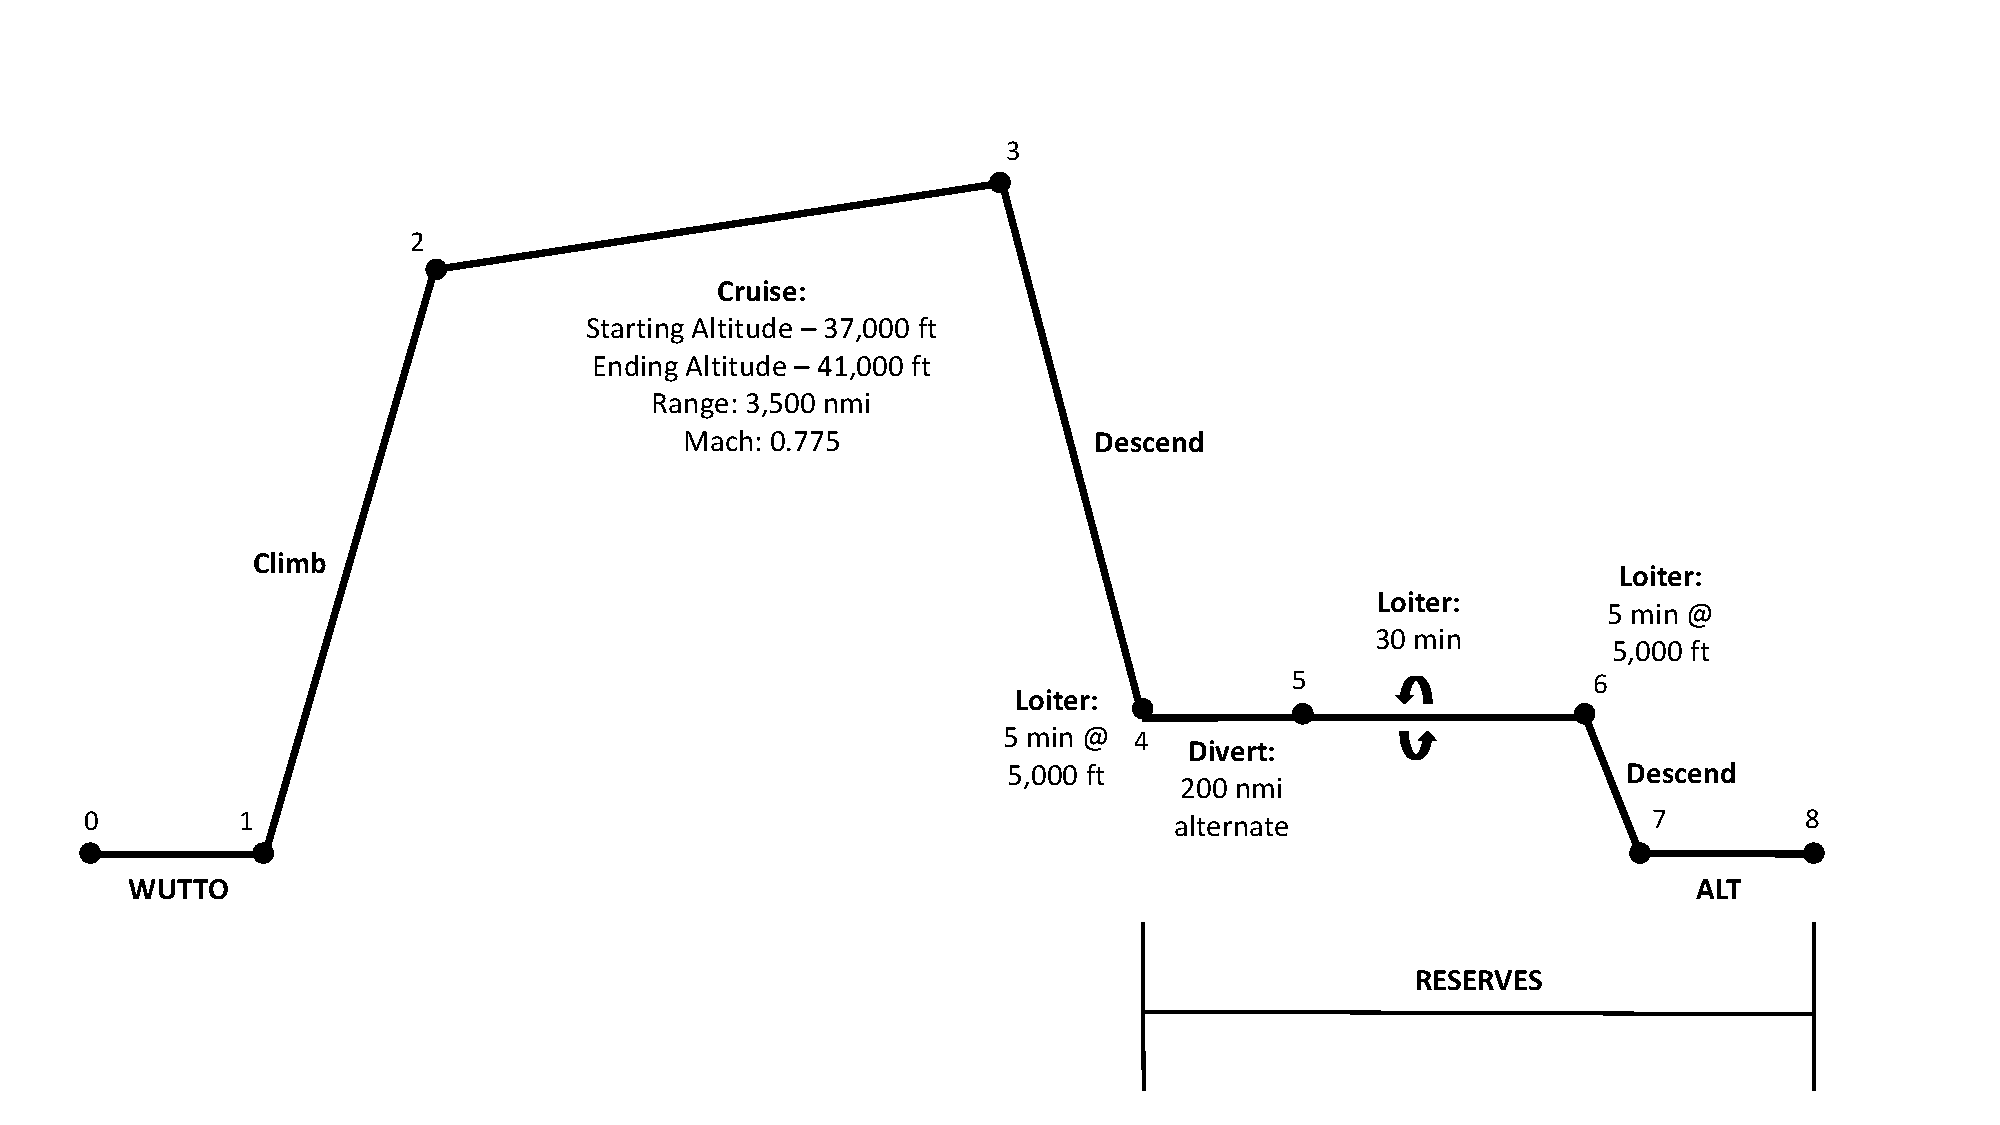
\includegraphics[width=1.0\textwidth]{Photos/Mission_Profile_(3-9-20).pdf}
    \caption{Typical Mission Profile}
    \label{fig:missionprof}
 \end{figure}

%\textcolor{red}{
%\begin{itemize}
    %\item AIAA: A description of the design missions defined for the proposed concepts for use in
%calculations of mission performance as per design objectives. This includes the
%selection of cruise altitude(s) and cruise speed/cruise Mach supported by pertinent
%trade analyses and discussion.
    %\item Discuss requirements (including those from the RFP and any additional derived requirements), constraints, and the design mission. \checkmark JJ
    %\begin{itemize}
        %\item Include a table of requirements.\checkmark JJ
        %\item \hl{Include a figure of the design mission with key mission segments labeled and details noted (e.g. cruise range and altitude).}
    %\end{itemize}
%\end{itemize}}

\clearpage
\section{Sizing Analysis (\textit{KP})}
\label{section: Sizing Analysis}
The initial sizing analysis was conducted by examining a variety of similar aircraft and making sure to satisfy all the requirements given by the AIAA RFP \cite{RFP}. Some of the analyzed aircraft included the Boeing 777-200, Boeing 787, Airbus A340-600, and the Lockheed L-1011-100, which all featured similar capacities and ranges. Once compiled, the aircraft were assigned a quantitative rank from one to seven based on  capacity and range. Sorting by composite score, the Boeing 777-200 was chosen as the main seed aircraft due to its highest perceived similarity to a hypothetical aircraft developed for the RFP \cite{RFP}. A seed aircraft is one whose major design characteristics are first used to help grow and fabricate what will become an iterative loop between major disciplines to find a balance that will become the final design.  Some key parameters derived from seed analysis and RFP mandates are presented in Table \ref{tab:req}; a list of all candidate aircraft considered in the sizing analysis is listed in Table \ref{tabmk1}, as the same subjects were used in the Section \ref{section: Configuration} trade study.

\begin{table}[h!] 
    \centering
    \caption{Key Sizing Parameters}
    \begin{tabular}{ |c||c| }\toprule
    \textbf{Parameter} & \textbf{Value} \\\hline\hline
    Payload & 94,000 [lb]  \\\hline
    Range & 3,500 [Nmi] \\\hline
    Takeoff Field Length with a 35 ft obstacle & 9,000 [ft]  \\\hline
    Landing Field Length & 9,000 [ft] \\\hline
    Cruise Speed & 487 [kts]\\\hline
    Cruise Altitude & 37,000 [ft] \\\hline
    Max Takeoff Weight & 364,626 [lb]\\\hline 
    L/D & 17.83 [$\sim$]\\\hline 
    $C_{L_{max}}$ & 1.65 [$\sim$]\\\hline 
    SFC & 0.65 [lb/lbf/hr]\\\hline 

    \end{tabular}\label{tab:req}
\end{table}

Parameters compiled from the similarity analysis were approximated by taking historic averages of those respective to the different analyzed aircraft. Preliminary cruise speed was obtained by assuming an average cruise Mach number of 0.9, while initial cruise altitude was estimated by taking averages of similar aircraft. Many other sizing parameters, specifically the wing geometries, were calculated using equations from Raymer \cite{raymer}. The wing area, however, was calculated by taking a couple averages of seed aircraft as an initial value of 4,600 ft$^2$. This value was used to determine other wing related parameters, and was fine tuned as the sizing process went along. With all estimated parameters, an iterative process was used with a sizing spreadsheet dynamically running through all of Raymer's \cite{raymer} fundamental sizing equations to converge all sizing values for the initial SAM Mk I. This step was necessary due to the significant differences in range from all contemporary widebody, 300+ capacity commercial aircraft which could have been used as a seed.

\clearpage
The aircraft's weights were calculated using two build up methods, instead of taking the seed aircraft's weights, by utilizing equations from Raymer \cite{raymer} and Roskam parts II \cite{roskam_2} and V \cite{roskam_5} and an initial assumption of 110,000 lb of fuel. A separate first-cut trade study was also conducted to address some key sizing parameters regarding the aircraft's fuselage to make sure that the SAM Mk I featured enough room for the designed seating arrangement. The trade study is demonstrated in Table \ref{tab:trade_params}.

\begin{table}[!h] 
    \centering
    \caption{Trade Study}
    \begin{tabular}{ |c||c||c| }\toprule
    \textbf{Aircraft} & \textbf{Fuselage Length [ft]} & \textbf{Max Takeoff Weight [lb]} \\\hline\hline
    Boeing 777-200 & 205.7 & 535,087  \\\hline
    Boeing 787-10 & 224.0 & 560,000  \\\hline
    Lockheed L-1011-100 & 177.8 & 466,079  \\\hline
    Airbus A340-600 & 228.2 & 390,307  \\\hline

    \end{tabular}\label{tab:trade_params}
\end{table}

After analyzing multiple aircraft, a fuselage length of 210 ft was decided in order to both hold more passengers than the Boeing 777-200 and to support a 3-4-3 economy seat arrangement. After utilizing a weight build up method, a max takeoff weight of 364,626 lb was calculated, which is about 200,000 lb heavier than the main seed aircraft. Once the weights were calculated, the total drag was able to be computed at desired takeoff conditions. This in turn allowed for a computation of required takeoff thrust to be about 71,500 lbf. 

\clearpage
% \textcolor{red}{\begin{itemize}
%     \item AIAA: A description or graphical representation of the aircraft sizing based on the
% requirements and design objectives given. \hl{This should describe or represent the
% quantitative justification for the wing area and thrust of the aircraft that was selected.} 
%     \item Discuss the team’s similarity analysis and the rationale behind the aircraft selection. \checkmark JJ
%     \item Discuss what data was extracted from the similarity analysis. \checkmark JJ
%     \item Discuss a part by part build up and how it compares to the seed analysis \checkmark JJ
%     \item Discuss initial sizing and constraint analysis. 
%     \begin{itemize}
%         \item Include a table of key parameters used with justification for their values. \checkmark JJ
%         \item Include at least takeoff, landing, cruise, service ceiling, and \hl{loiter constraints.}
%     \end{itemize}
%     \item Include at least two trade studies that uses quantitative analysis to support design decisions made. \hl{I split into the sizing \& then fuse sizing as the "second" one}  Maybe tie into the trade study Mat outlined right below? I put a possible bridge in the first paragraph to it if you want to go that route. 
%     \item Include the aircraft allocated and derived requirements and their justifications: \hl{(I think he might want this for all of the aircrafts we used? Open to interpretation)}
%     \begin{itemize}
%         \item $\frac{L}{D}$
%         \item $C_{L,max}$
%         \item SFC
%         \item Weights
%     \end{itemize}
% \end{itemize}}

% \clearpage
\section{Configuration (\textit{MK})}
\label{section: Configuration}
\subsection{External Configuration  (\textit{MK})}
Many configurations of aircraft were considered during initial design phase. First, a trade study was performed over similar aircraft that are either currently in service or have flown in the past. Table \ref{tabmk1} describes seven aircraft and some of their prominent external configuration characteristics. 

\begin{table}[!h]
    \centering
    \caption{Quantitative Trade Study of Similar Aircraft}
    \begin{tabular}{|m{2cm}||c|c|c|c|c|}
    \toprule
    \label{tabmk1}
    \textbf{Aircraft} & \textbf{Tail Type} & \textbf{Wing Type} & \textbf{\# of Engines} & \textbf{2-class Seating} & \textbf{Deck Layout} \\
    \hline\hline
    B777-200 & Conventional & Low & 2 & 375 & Single \\ 
    \hline
    A340-600 & Conventional & Low & 4 & 440 & Single \\
    \hline
    B787-10 & Conventional & Low & 2 & 330 & Single \\
    \hline
    MD-11 & Conventional (w/ engine) & Low & 3 & 323 & Single \\
    \hline
    L1011-100 & Conventional (w/ engine) & Low & 3 & 304 & Single \\
    \hline
    B747-400 & Conventional & Low & 4 & 496 & Double \\
    \hline
    A350-900 & Conventional & Low & 2 & 315 & Single \\
    \bottomrule
    \end{tabular}
\end{table}
\clearpage
From the trade study, all seven of described aircraft feature a low wing along with a conventional tail. This is most likely due to the low wing providing space for a retractable landing gear along with simplicity of design. Thus, the team decided to go with a low wing.

The next external configuration decision was between a T-tail and a conventional tail. While the T-tail does reduce the risk of the tail stalling, it is much more difficult to design as the vertical tail has to support the entire weight of the horizontal tail. Alternatively, conventional tails are lighter and provide more simplicity in terms of design. Another benefit of conventional tails is that it allows for easier implementation of control surfaces to the aircraft. Additionally, the team had already decided to utilize wing mounted engines, which provides more resistance from the wing bending too much and saves on structural weight of the wing. As shown from the trade study, conventional tails are very widely used in similar configuration commercial aircraft in today's market; thus the team decided to use a conventional tail configuration as illustrated in Figure \ref{fig:threeview}.

Next, the number of engines on SAM Mk. 1 along with the number of decks on the aircraft remained to be decided. The team decided to go with a single-level to provide simplicity in design as well reduced cost in manufacturing. Furthermore, two engines were chosen for SAM Mk. 1, mainly for the reduced maintenance cost, reduced cost in total price of engines for the aircraft (four engines typically cost more than two engines), and an assumed low cost of fuel. The proven reliability of modern engines in trans-oceanic flights also played a role in deciding to have two engines. Finally, the landing gear of our aircraft was determined to be a retractable, tricycle configuration further discussed in Section \ref{section: Landing Gear}. 

Figure \ref{fig:threeview} shows a top, left, front, and isometric view of the CAD model of the aircraft. The SAM Mark 1 has a total length of 233 ft, 4 in and a wingspan of 184 ft, 5 in. The coordinate system for the aircraft starts at the tip of the nose cone of the aircraft, with the x-direction pointing out of the coordinate system, y-direction in the direction of the right wing, and z-direction down. Moreover, Figure \ref{grndline} shows the ground line of the aircraft with the landing gear extended.

\newpage

\begin{figure}[H]
    \centering
    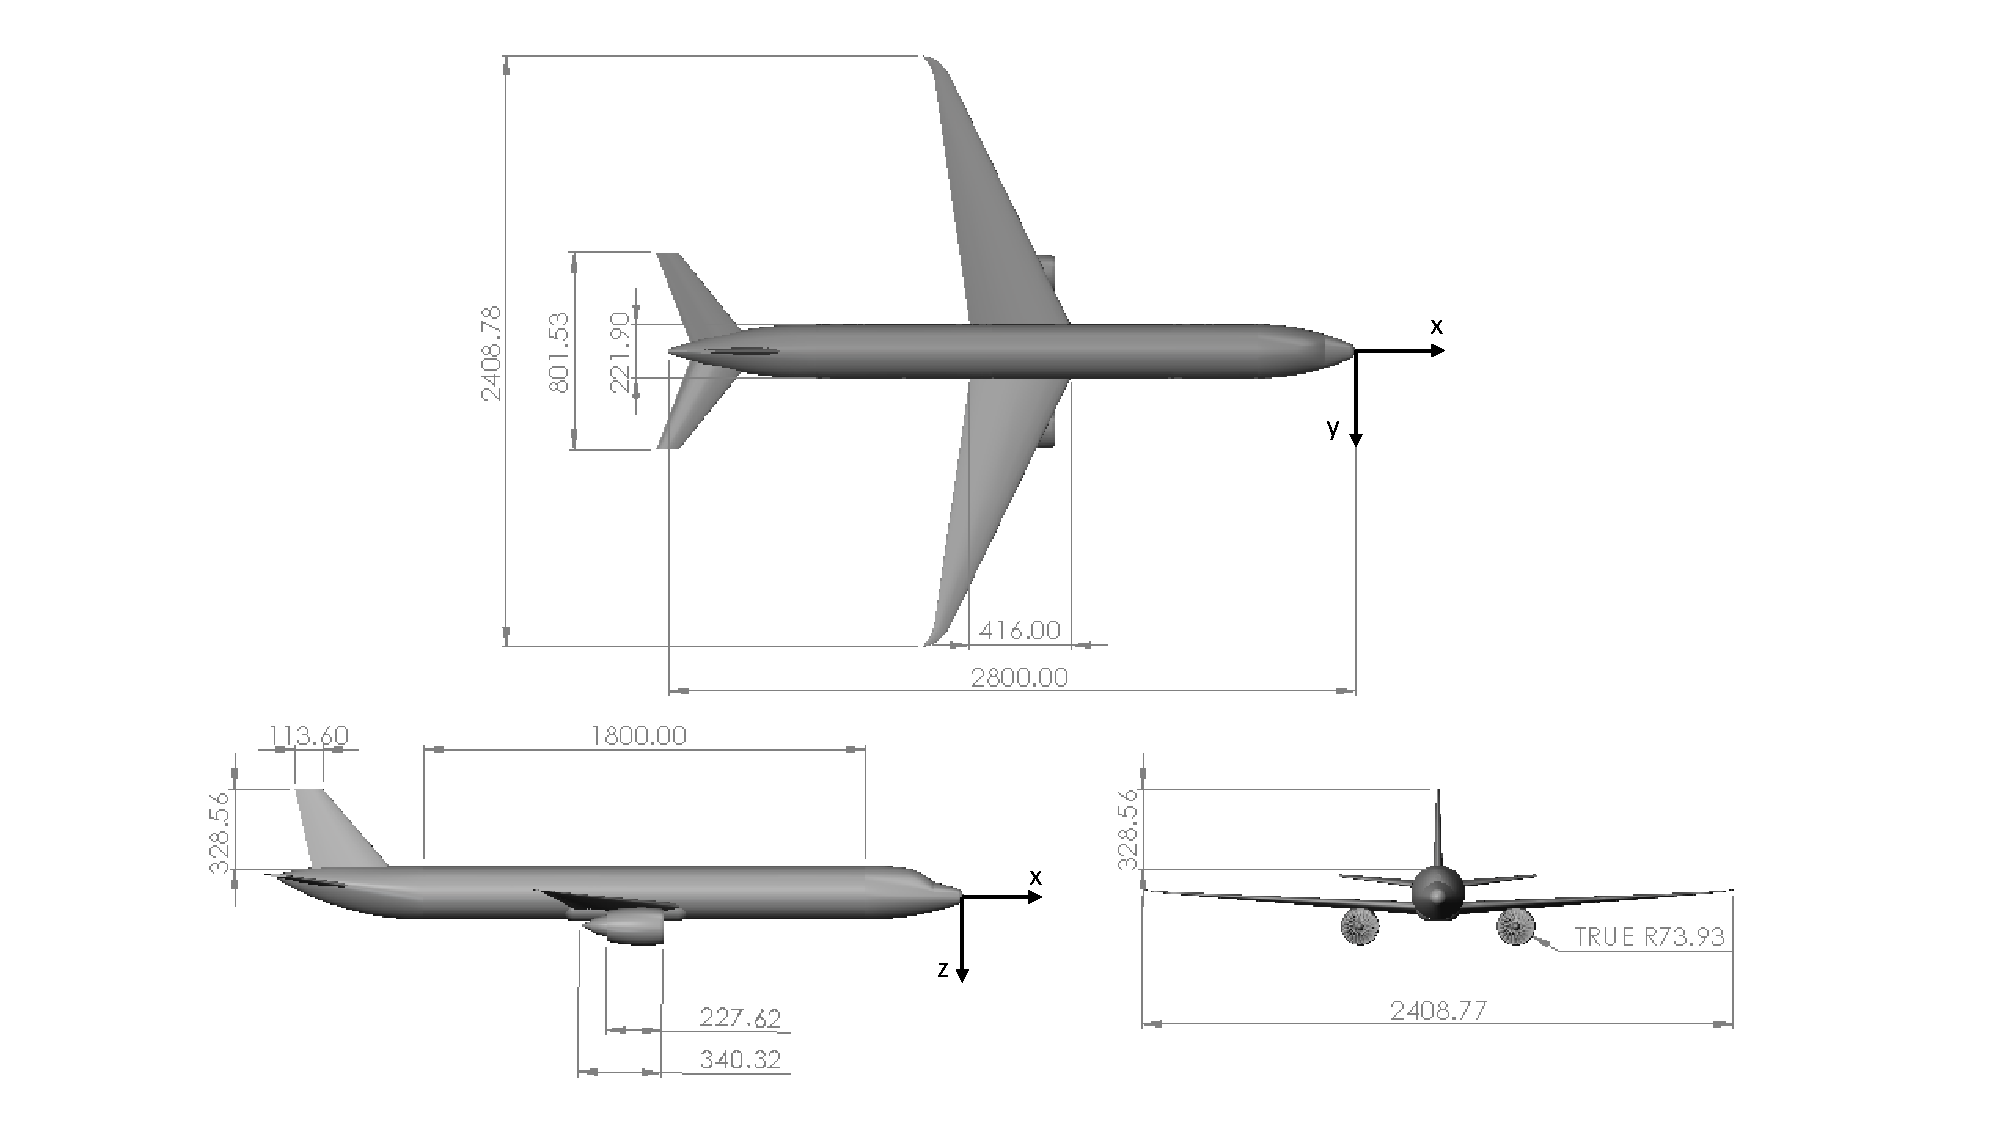
\includegraphics[width=1.4\linewidth, angle =90 ]{Photos/3-view_with_coords.pdf}
    \caption{3-View Drawing of SAM Mark 1 [in]}
    \label{fig:threeview}
\end{figure}
\clearpage

\begin{figure}[!h]
    \centering
    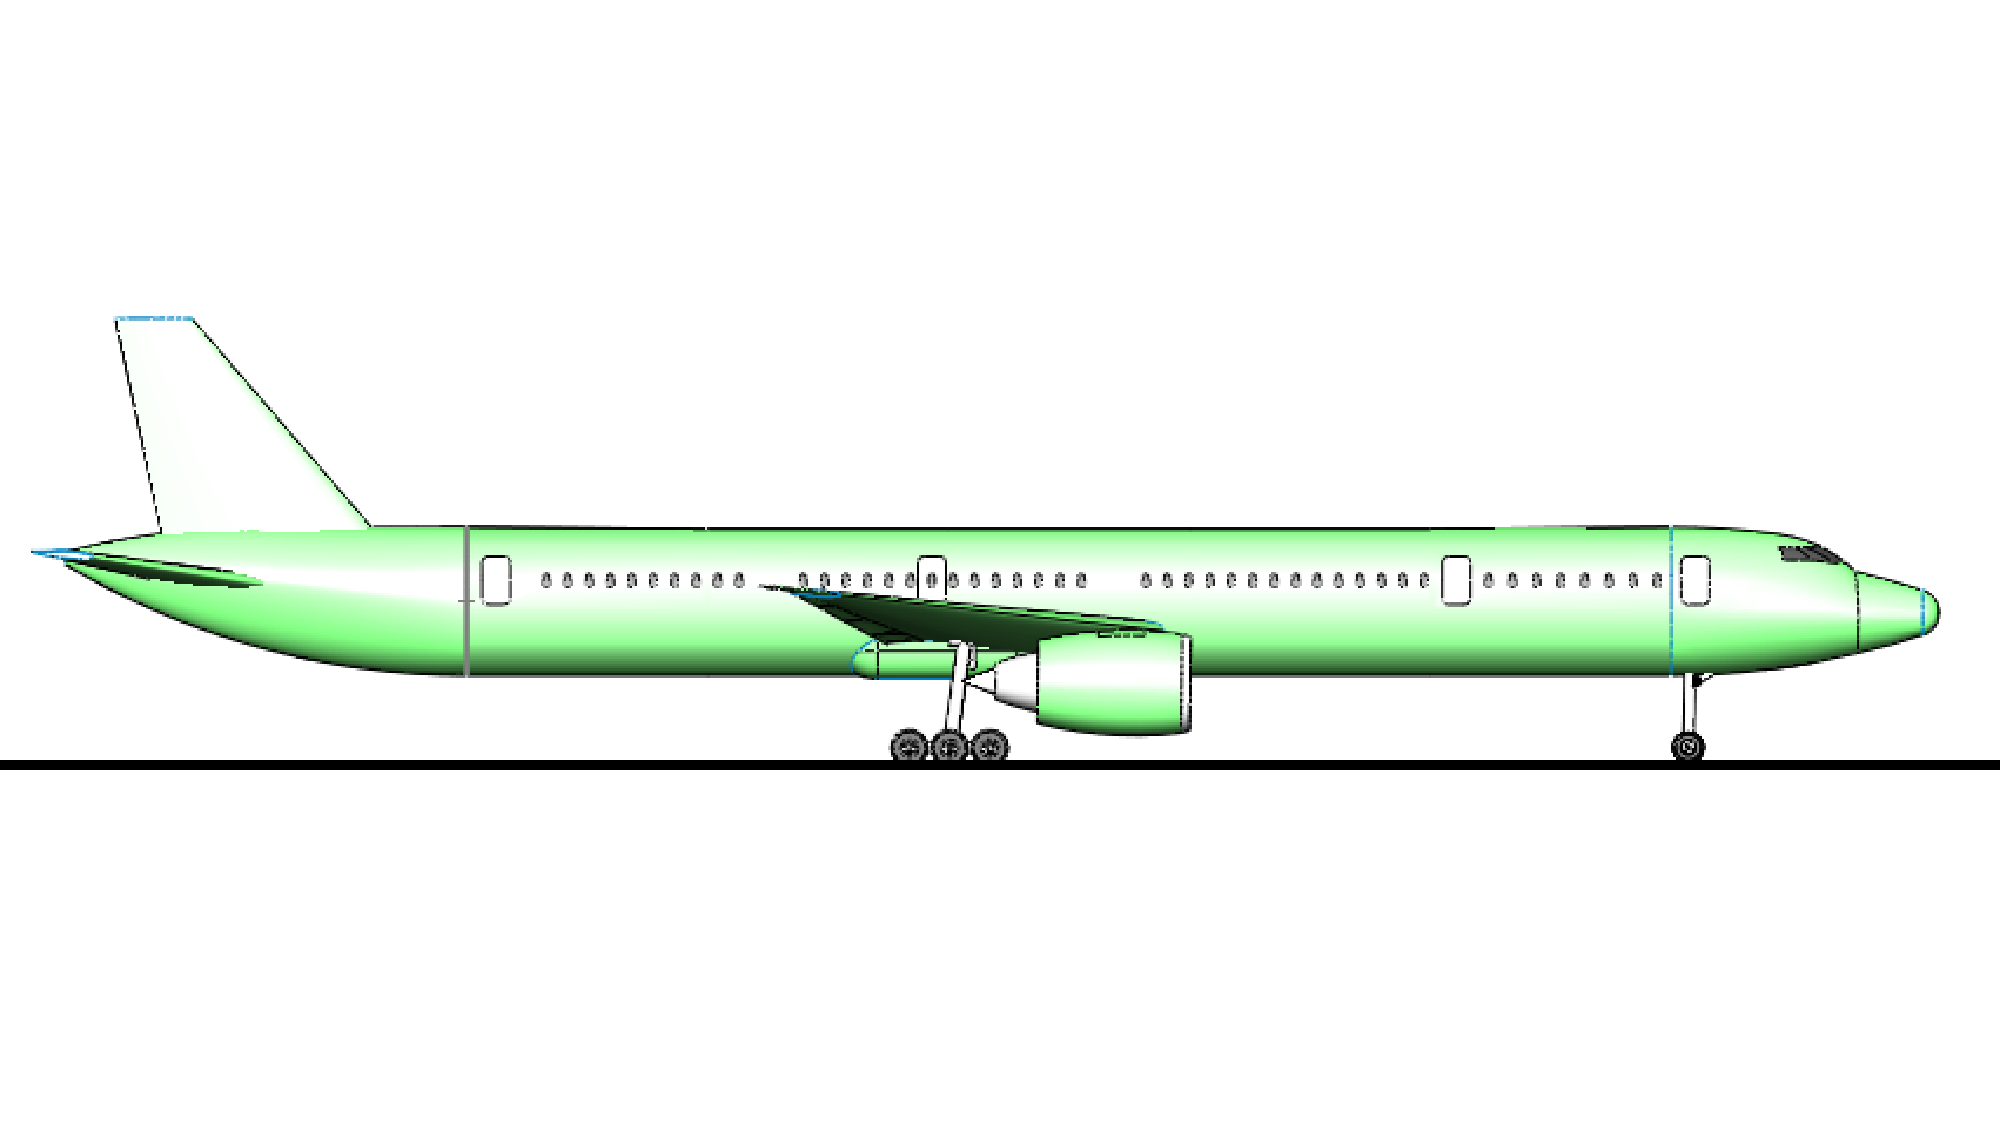
\includegraphics[width=1.0\textwidth]{Photos/Ground_Line.pdf}
    \caption{Side View of SAM Mk. 1 with Ground Line}
    \label{grndline}
 \end{figure}

\subsection{Internal Configuration (\textit{JC})}
\label{section: internal config}
\subsubsection{Flight Deck Configuration}
The flight deck is configured for two pilots.  Adjustable seats enable ease of access to control panels the flight deck includes seating accommodation for two pilots, traditional of most commercial aircraft.  

\subsubsection{Seating Configuration (JC)}
The aircraft internal configuration is presented as two-class seating combining both business and economy seating accommodations.  Per AIAA RFP \cite{RFP} requirements, the aircraft is designed with 50 business-class and 350 economy-class seats to accommodate 400 total customers.  

\begin{table}[!h]
    \centering
    \caption{Seating Configuration}
    \begin{tabular}{|c|c||c|c|} \toprule
        \multicolumn{2}{c}{\textbf{Business Class}} & \multicolumn{2}{c}{\textbf{Economy Class}} \\ \hline
        Configuration (a) & 2 - 2 - 2 & Configuration (a) & 3 - 4 - 3 \\ \hline
        Row Count (a) & 8 & Row Count (a) & 28 \\ \hline
        Configuration (b) & 1 - 0 - 1 & Configuration (b) & 2 - 3 - 2 \\ \hline
        Row Count (b) & 1 & Row Count (b) & 10 \\ \hline
        Pitch & 36 [in] & Pitch & 32 [in] \\ \hline
        Width & 21 [in] & Width & 18 [in] \\ \bottomrule
    \end{tabular}
    \label{tab:seating}
\end{table}

Two different seating configurations are proposed for each class in Table \ref{tab:seating}, above.  The business class contains 8 rows with a 2 - 2 - 2 configuration to provide a spacious flight experience while making efficient use of the space provided.  The purpose of selecting a 2 - 2 - 2 style is to provide business passengers the opportunity to have aisle access.  The 1 - 0 - 1 row is provided to accommodate ADA passengers \cite{adaseating} and may be further customized by the client.  The economy class has two sections with a 3 - 4 - 3 and 2 - 3 - 2 configuration.  The 3 - 4 - 3 section provides high capacity seating while the 2 - 3 - 2 seating enables airliners to offer a highly competitive yet still profitable seating arrangement.

\begin{figure}[!h]
    \centering
    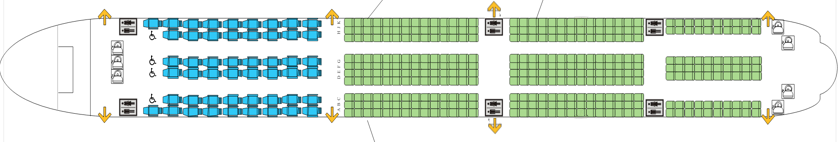
\includegraphics[width=0.7\textwidth]{Photos/Config undimensioned.png}
    \caption{Internal Configuration}
    \label{fig:internalConfig}
\end{figure}

Crew seating can be oriented per customer request in the front and aft galleys and complies with 14 CFR \S 121.391(d).

\subsubsection{Galley Configuration}
SAM Mk 1 provides 2 galley locations, at the front and rear sections of the cabin.  This configuration optimizes crew capability of evenly servicing the two classes with minimal cross traffic.  By using the front entrance and aft sections of the cabin for galley and flight crew seating, there is 20 $ft^2$ of available space for airline partners to customize the galley sections to fit specific needs.

\subsubsection{Lavatory Configuration}
SAM Mk 1 offers up to 6 lavatories in its 3,500 Nm configuration to provide ease of access and mitigate aisle traffic.  Each lavatory is equipped with internal lighting, toilet facility, sanitation wipes, ash tray, emergency assistance button, and trash bin.  A sink and hand soap dispenser may be included per customer request; though sanitation wipes are provided as a weight saving measure.  The toilet facility uses negative pressure vacuum disposal system to vacate contents into a disposal tank stowed in the aft of the fuselage.\cite{toilet}  Lavatory doors are designed to lock from both the interior and the exterior for security.  Flight crew may be provided the key access to lock the lavatory doors from the exterior if a member on-board violates 14 CFR 91.11, 121.580, 135.120, 125.328, 49 USC 46318 \& 46504.

Configuration of lavatory may be modified to fit airline partner's needs.

\subsubsection{Door Configuration}
Sam Mk 1 provides 4 pairs of emergency doors, pursuant to 14 CFR 25.807.  The front and aft emergency exits are a minimum of 24 inches wide and 48 inches high and when unlocked and activated, translates outwards and along the side of the fuselage.  The method of opening the emergency door is to allow maximum door clearance without requiring special boarding adapters from the jet bridge \cite{cfr}.








% \textcolor{red}{
% \begin{itemize}
%     \item Discuss external configuration alternatives considered and design choices made.
%     \begin{itemize}
%         \item \hl{Include a morphology wherein primary design alternatives are shown (via OpenVSP visual) and discussed (i.e. advantages/disadvantages) for different areas of consideration (i.e. wing placement, engine placement).}
%     \end{itemize}
%     \item Discuss selected aircraft configuration design (i.e. distinctions between variants, major features, design characteristics/objectives).
%     \begin{itemize}
%         \item \hl{Include a scaled 3-view drawing as comprehensive visuals that detail all major dimensions and parameters of the external configuration.}
%         \item \hl{Use a separate foldout for the 3-view.}
%         \item \hl{Show dimensions for: length, height, CG, and neutral point of entire aircraft; span, root and tip chord for wings, vertical tail, horizontal tail/stabilizer, flaps, ailerons, elevators, and rudder; length and diameter (width and height if non-circular) for fuselage and inlet(s); width and height of major door; height of landing gear.}
%         \item \hl{Show an overlay (dotted) of stowed landing gear (if applicable)}
%         \item \hl{Show ground lines.}
%     \end{itemize}
%     \item \hl{Discuss internal configuration design to meet objectives (i.e. customer appeal) and requirements (i.e. baggage capacity). !!!! for Josh to do}
%     \begin{itemize}
%         \item \hl{Include internal configuration drawing.}
%         \item \hl{Show dimensions for: cabin length, cabin width, cabin height, aisle width, passenger seats' length and width, width of door, and baggage compartment length and width.}
%     \end{itemize}
%     \item Include at least one trade study that uses quantitative or qualitative analysis to support design decisions made.
%     \item Discuss the landing gear philosophy.
%     \item 3-View drawing (VSP acceptable).
%     \item Discuss future work
%     \item AIAA: Complete geometric description, including dimensioned drawings, control surfaces sizes and hinge locations, and internal arrangement of the aircraft illustrating sufficient volume for all necessary components and systems to fulfill \#7 as seen \href{https://www.aiaa.org/docs/default-source/uploadedfiles/education-and-careers/university-students/design-competitions/undergraduate-team-aircraft-design-competition/undergraduate-aircraft-high-capacity-short-range-transport-aircraft.pdf?sfvrsn=b6081273_0}{here}: )
% \end{itemize}}

\clearpage
\section{Propulsion (\textit{NZ})}
\label{section: Propulsion}



In order to create a basis for the engine choice, a trade study was performed on the engines of similar aircraft. These aircraft, such as the Boeing 777-300, Airbus A330-300, Airbus A330-900, and Airbus A350 XWB, have a similar passenger capacity as the one required in the design competition, however all have a much higher range capability. The primary drivers for the design of the propulsion system are the power requirement for the aircraft, as well as reliability. Since the aircraft will be used as a high capacity transport for short mission durations, it is vital that the engines can withstand a constant cycle of maximum take off thrust at a higher interval than tradition engines which experience longer flight durations. 

\subsection{Engine Comparisons}

The following engines, seen below, are used in similar aircraft with great success: Pratt \& Whitney PW4000, General Electric GE90-115B, Rolls-Royce Trent XWB, and Rolls-Royce Trent 7000.

\begin{table}[!h]
    \centering
        \caption{Comparison of Engines on Similar Aircraft}
    \begin{tabular}{|c||c|c|c|c|}\toprule
         & \textbf{PW4000} & \textbf{GE90-115B} & \textbf{RR Trent XWB} & \textbf{RR Trent 7000} \\\hline \hline
         \textbf{Aircraft} & Airbus A330-300 & Boeing 777-300 & Airbus A350 XWB & Airbus A330-900\\ \hline
         \textbf{Maximum Takeoff Thrust [lb]} & 52,000 - 62,000 \cite{PW} & 110,000  \cite{ge90} & 84,200  \cite{xwb} & 71,110  \cite{butterworth}\\ \hline
         \textbf{Dry Weight [lb]} & 12,900  \cite{FAApw} & 19,316  \cite{ge90} & 16,043  \cite{xwb2} & 10,550 \cite{butterworth} \\ \hline
         \textbf{Cost per Unit [USD]} & - & \$ 27.5 million \cite{gecost} & - & \$ 11 million \cite{butterworth} \\ \hline
         \textbf{Bypass Ratio} & 4.9 : 1 \cite{PW} & 9 \cite{safran} & 9.6 : 1 \cite{xwb} & 4.89 : 1 \cite{butterworth} \\ \hline
         \textbf{Fan Diameter [in]} & 94 \cite{PW} & 135 \cite{ge} & 118 \cite{xwb} &  97 \cite{butterworth}\\ \hline
         \textbf{SFC [lb/lbf/hr]} & 0 & 0.545 \cite{butterworth} & 0 &  0.565 \cite{butterworth} \\ \hline
         \textbf{Thrust to Weight} & 4.80-4.03 & 5.69 & 5.24 & 6.74 \\ \bottomrule
    \end{tabular}
    \label{tab:enginecomp}
\end{table}


While the aircraft are similar in capacity, the range on these aircraft is much higher than what is required for the SAM Mk I. As such, an assumption is made that the engines chosen for these aircraft may not be as reliable as necessary for the SAM Mk I, since the engine for the SAM Mk I will experience higher intervals and much more frequent cycling of maximum thrust, leading to more fatigue to the engine. 

In order to validate the choice of a turbofan engine, which was also the type of engine of choice for the similar aircraft compared above, Figure \ref{PropSelection} was used along with the Mach speed the SAM Mk I will fly at cruise conditions, 0.775. This figure was used to quickly determine which propulsion systems are overpowered for the flight conditions that the aircraft will fly and rule out which propulsion systems would not be able to meet the flight conditions \cite{raymer}.

\begin{figure} [h!]
    \centering
    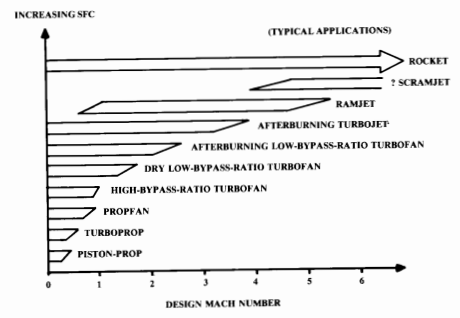
\includegraphics[width=0.8\textwidth]{Photos/PropSelection.PNG}
    \caption{Propuslion System Speed Limits}
    \label{PropSelection}
\end{figure}

\newpage
With a Mach number of 0.775, both piston-prop and turboprop engines are not able to meet the speed requirement for cruise. The propfan propulsion system, while it may be able to handle a Mach number of 0.775, is not ideal as it is operating at the end of its limit. Scramjet and ramjet propulsion systems are over powered for the SAM Mk I system, leaving only three classes of turbofan engines and an afterburning turbojet engine. According to Raymer, the propulsion system should be one which the lowest on the chart for the specified Mach number, which for this case is the high-bypass-ratio turbofan \cite{raymer}. In addition, all of the engines listed in Table \ref{tab:enginecomp} are high-bypass-ratio turbofan propulsion systems as well, which gives confidence in the high-bypass-ratio turbofan engine being the propulsion system of choice for the SAM Mk I, barring any critical design concerns.

\subsection{Engine Requirements}

Using the sizing analysis in which a similar aircraft was seeded into, several of the specifications of the SAM Mk I were inputted in order to obtain a thrust requirement for the aircraft. The sizing analysis estimated that the SAM Mk I would require a thrust of 151,000 lb.

Furthermore, an engine with high reliability was sought after due to the high cycling behaviour of take-off that this aircraft will see. Therefore, an engine which has already undergone certification and has been in service with a proven track record of reliability was prioritized.

\subsection{Engine Selection}

The engine of choice for the SAM Mk I will be General Electric's GE90-115B. The selection of this engine was driven by the desire to have an engine that is already in service and has a proven track record of reliability.

\begin{table}[!h]
    \centering
        \caption{GE90-115B Specifications}
    \begin{tabular}{|c||c|}\toprule
         & \textbf{GE90-115B} \\\hline \hline
         \textbf{Maximum Continuous Thrust [lb]} & 110,000  \cite{ge90} \\ \hline
         \textbf{Take-off Thrust (5 minutes) [lb]} & 115,540  \cite{ge90} \\ \hline
         \textbf{Dry Weight [lb]} & 19,316  \cite{ge90}  \\ \hline
         \textbf{Cost per Unit} &  \$ 27.5 million \cite{gecost}  \\ \hline
         \textbf{Bypass Ratio} & 9 \cite{safran}  \\ \hline
         \textbf{Fan Diameter [in]} & 135 \cite{ge} \\ \hline
         \textbf{Engine Length [in]} & 286.7 \cite{ge} \\ \hline
         \textbf{Engine Width [in]} & 148.4 \cite{ge} \\ \hline
         \textbf{Engine Height [in]} & 154.6 \cite{ge} \\ \hline
         \textbf{Thrust to Weight} & 5.69 \\ \bottomrule
    \end{tabular}
    \label{tab:GE90}
\end{table}

The unit cost for this engine was approximately \$27.5 million dollars in 2011 \cite{gecost}. When accounting for inflation, the current price is \$31.5 million dollars. Assuming an average rate of inflation of 3\% a year, the estimated cost of this engine once the SAM Mk I goes into service in 2029 will be approximately \$ 47 million dollars.

\begin{figure} [h!]
    \centering
    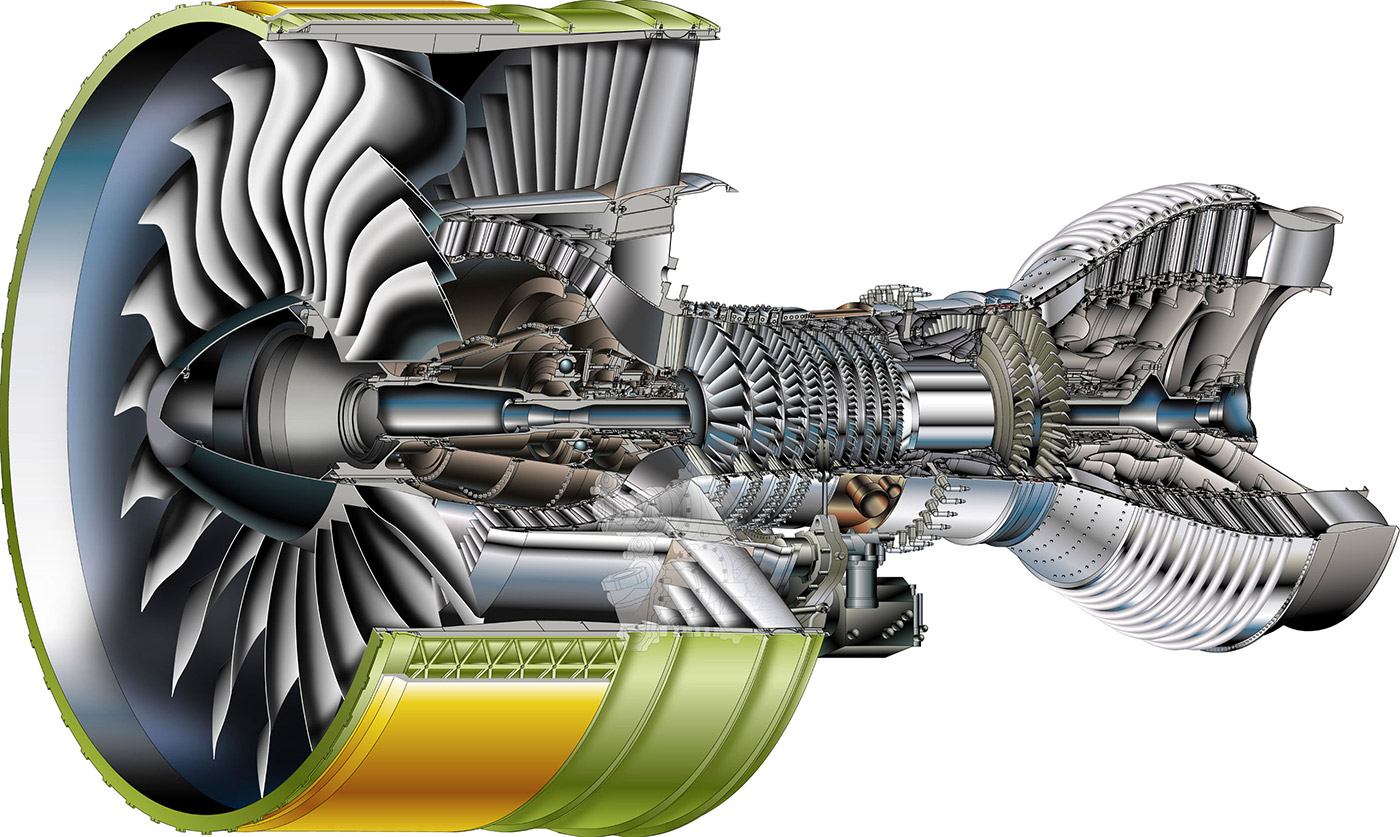
\includegraphics[width=0.8\textwidth]{Photos/ge90cross.jpg}
    \caption{Cross-section of the GE90-115B}
    \label{fig:GeCross}
\end{figure}

The GE90-115B is a dual rotor, high bypass ratio turbofan. It has a 9 stage high pressure compressor that is followed by a 2 stage high pressure turbine. Continuing, a 6 stage low pressure turbine drives the 4 stage low pressure compressor as can be seen in Figure \ref{fig:GeCross} \cite{gecross}. This engine had the first ever composite fan blades in commercial aviation that allowed it to be one-third the weight of industry standard titanium blades at the time. It is also quieter and more efficient than most other engines in it's thrust class \cite{ge90}.

The GE90-115B has its gearbox located on the underside of the wing where all other engine accessories such as fuel pumps, oil pumps, and engine control boxes are stored as well. Although no sources have confirmed this location, according to Raymer, it is the most likely location of the the accessory package \cite{raymer}.

% \textbf{plagiarized} The "bypass ratio" is the mass-flow ratio of the bypassed air to the air
% that goes into the core 'of the engine \cite{raymer} To lower the temperature seen by the turbine blades, excess air is used. Currently engines are limited to a turbine temperature of about 2000-25000F, which requires an air/fuel mixture ratio of about 60 to 1. Thus,
% only about a quarter of the captured and compressed air is actually used for
% combustion. The exhaust is 75 \% unused hot air

% Note the engine-accessories package beneath the engme. The accessones
% include fuel pumps, oil pumps, power-takeoff gearboxes, an~ engine control boxes. The location and size of the accessory package vanes widely for
% different types of engines. In the absence o~ a drawing: the accessory package can be assumed to extend below the engine to a radius of a~out 20-400Jo
% greater than the engine radius. On some engmes these accessories have been
% located in the compressor spinner or other places


\subsection{Validation of Engine Choice}

Since the GE90-115B engine is rated to approximately 115,000 lbs of thrust per engine, in case of an engine-out system, the engine would still be able to provide more than 50\% of the estimated required thrust in order to keep the plane in flight. This offers an extra level of safety than if a lesser thrust rated engine was chosen who would not be able to provide such a high percentage of necessary thrust. Furthermore, the GE90-115B has a very strong safety record, with it having a reported in-flight shutdown rate of one per million engine flight hours \cite{geifsd}. 

\begin{figure} [h!]
    \centering
    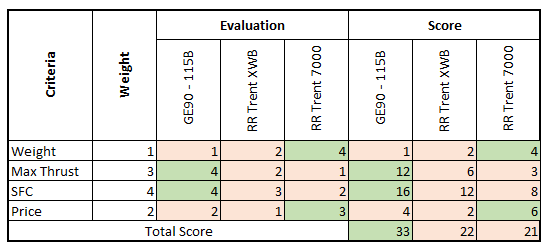
\includegraphics[width=0.8\textwidth]{Photos/GE90Trade.PNG}
    \caption{Engine Trade Study}
    \label{fig:enginetrade}
\end{figure}

\begin{figure} [h!]
    \centering
    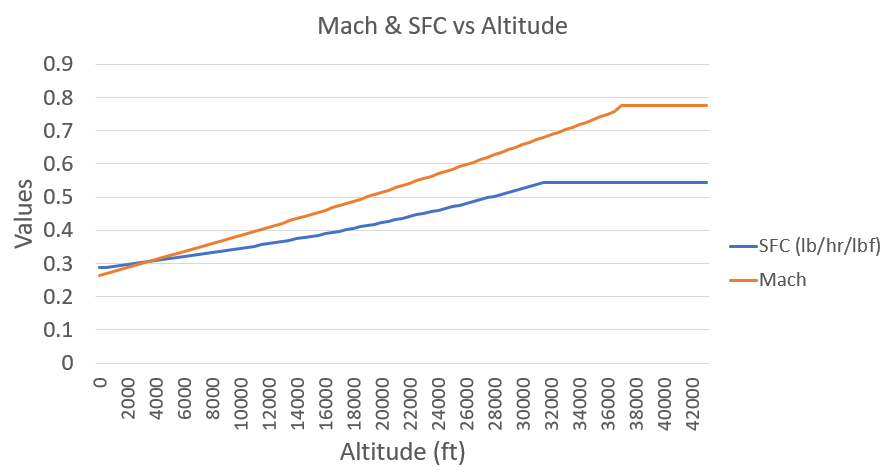
\includegraphics[width=0.8\textwidth]{Photos/machvssfc.PNG}
    \caption{Mach and SFC vs Altitude of the GE90 - 115B}
    \label{fig:machvssfc}
\end{figure}

\begin{figure} [h!]
    \centering
    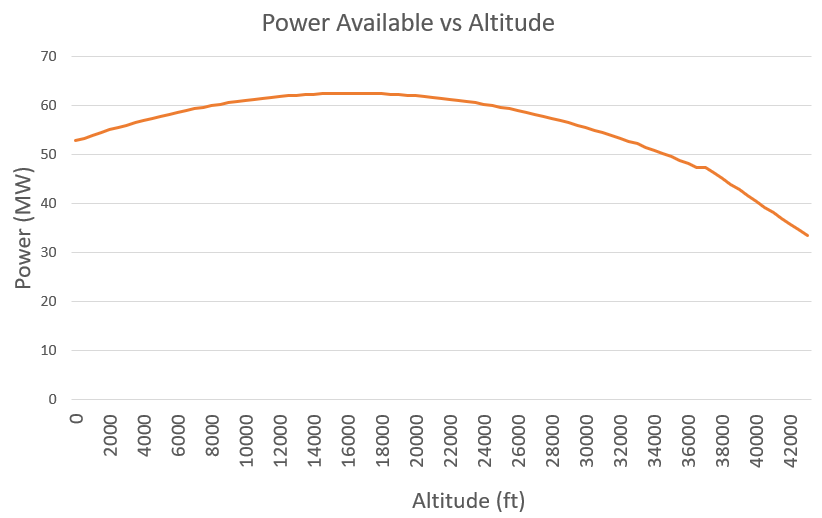
\includegraphics[width=0.8\textwidth]{Photos/powervsaltitude.PNG}
    \caption{Power Available vs Altitude for the GE90 - 115B}
    \label{fig:poweravailable}
\end{figure}

A trade study was conducted which validated the choice of the GE90-115B. Four main categories were considered: price, SFC, weight and maximum thrust. The maximum thrust and SFC were weighted the heaviest due to the primary driver of reliability and safety. A higher maximum thrust allows greater safety in case one engine fails since the thrust lost will not be as significant. Through all of these considerations, it can be seen that the GE90-115B is the best choice.

\subsection{Inlet, Nacelle/Pod Covers and Exhaust Design}

The engines will be located, one of each side, underneath the wings of the aircraft. This is beneficial for a multitude of reasons, however it is primarily helpful in case of an emergency water landing. Due to the high weight of the engines, when the engines are located under the wing, they will be sheared off on impact during an emergency water landing. With the loss of this heavy, and very dense weight, the aircraft now can float for a longer period of time, allowing passengers more time to reach the safety of lifeboats and evacuate. Other engine mountings were not considered due to noise concerns, controllability \ stability in case of engine-out, or due to other safety considerations such as the one mentioned above. Wing mounted engines also have several benefits such as distributing the weight across the wings and the use age of the flaps on the wings can greatly increase lift \cite{raymer}.



The inlet, nacelle cover, and exhaust design were borrowed heavily from the Boeing 777-200, due to the aircraft's similarity to the SAM Mk I. However, some design considerations were taken from Raymer: namely, the nacelle will be angled down by 3 degrees as recommended by \cite{raymer}. In order to have the most efficient turbofan engine as possible, the air entering the engine must be at a Mach of 0.4-0.5 and therefore needs to be slowed down when in flight. This is done by the geometry of the inlet which causes a pressure less and therefore direct increase in the thrust generated by the engine. 

The most simple and straightforward inlet is the pitot inlet which would work very well for the SAM Mk I.

\begin{figure} [h!]
    \centering
    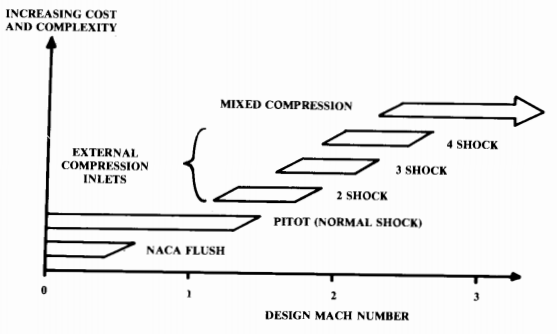
\includegraphics[width=0.8\textwidth]{Photos/inletapplicability.PNG}
    \caption{Inlet Geometry Choice vs Mach}
    \label{fig:inlet}
\end{figure}

% diffuser design? I don't wannna. the diffuser should be as
% short as possible without exceeding an internal angle of about IO deg. Typically, this produces a pitot inlet with a length about equal to its front-face diameter

\subsection{Future Progress}

Although the gas turbine engine is the superior choice for this aircraft from intuition and the current progress of electric motors, in the future it would be beneficial to calculate the energy density of batteries and electric motors and compare it to the energy density of a gas turbine engine in order to definitively rule out electric propulsion. Due to the weight and bulk of such systems, no trade study was run, however having quantitative analysis in order to prove the the incapability of such a system for a commercial aircraft.

Further work can also be done on the inlet, nacelle/pod/covers, and exhaust design. Currently, the design borrows heavily from the Boeing 777 due to the aircraft's similarity to the SAM Mk I. However, it would be a good idea to further refine the design in order to improve it's performance on the SAM Mk I.

\hl{maybe rename to later considerations or something like that for FDR purposes}

\section{Crap to Add}

Add in engine de-rating. Validate using CFR using oversized engine. Fix plots

% \textcolor{red}{
% \begin{itemize}
%     \item AIAA: Propulsion system description and characterization including performance,
%     dimensions, and weights. The selection of the propulsion system(s), sizing, and
%     airframe integration must be supported by analysis, trade studies, and discussion
% \end{itemize}}


% \textcolor{red}{
% \begin{itemize}
%     \item Discuss overall propulsion system design.
%     \begin{itemize}
%         \item Discuss engine requirements (e.g. power and thrust required) and selection.
%         \item Discuss architecture and configuration (e.g. sub-system placement).
%         \item Discuss safety considerations (i.e. engine-out)
%     \end{itemize}
%     \item Discuss main powerplant selected, including decision process, specifications, and performance data (e.g. power available vs altitude vs. Mach, SFC vs. altitude vs. Mach).
%     \item Discuss inlet, nacelle/pod/covers, and exhaust design.
%     \begin{itemize}
%         \item Include basic integration (CAD if using nacelles/pod/covers, general location and spacing if integrated into fuselage).
%         \item Include inlet and exhaust design (e.g. areas, routing).
%         \item Include inlet performance (e.g. pressure losses, install power).
%     \end{itemize}
%     \item Include at least one trade study that uses quantitative or qualitative analysis to support design decisions made.
% \end{itemize}}

\clearpage
\section{Aerodynamics (\textit{JC})}
\label{section: Aerodynamics}
\subsection{Airfoil Analysis}
The desired cruise conditions of Mach 0.775 and wing Reynolds number 4x$10^7$ for the aircraft fall within the transonic speed regime.  While this provides favorable conditions for the sizing analysis, the effects of wave drag increase as the aircraft approaches supersonic regime.  As shown in Figure \ref{fig:transonic}, the effects of wave drag is observed to increase as Mach increases \cite{raymer}.  Comparable aircraft combine use of supercritical airfoil and quarter chord sweep angles to delay the separated boundary layer due to shock.  Therefore, a selection of supercritical airfoils and wing sweep of no less than $32\degree$ is proposed to mitigate the increased effects of wave drag.

\begin{figure}[!h]
    \centering
    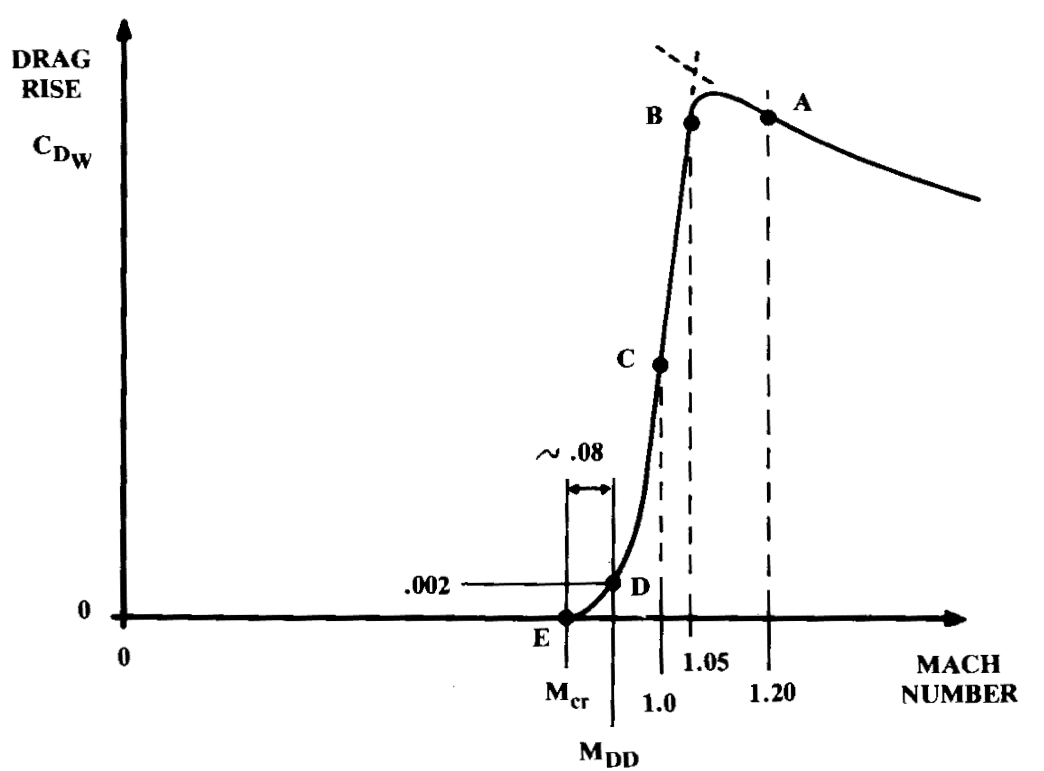
\includegraphics[width=0.65\textwidth]{Photos/wavedragduetotransonic.png}
    \caption{Wave Drag due to Transonic Airspeed\\{\small From Raymer Fig. 12.29}}
    \label{fig:transonic}
\end{figure}

\subsubsection{Airfoil Trade Study}
A trade study is conducted comparing the fundamental characteristics between NACA 5-series airfoils and NASA supercritical airfoils.  Information learned in a NASA study \cite{supercritical} demonstrated the benefits of supercritical airfoils in delaying $M_{DD}$ such the wave drag is mitigated.  Consequently, several supercritical SC(2)-series airfoils, illustrated in Figures \ref{fig:0412airfoil} - \ref{fig:0712airfoil}, are selected and compared.  Using XFLR5 \cite{xflr5} incompressible flow analysis for take-off conditions, a simulation is processed to provide numerical data.  The results of some preliminary analyses through XFLR5 are listed below in Figure \ref{fig:airfoils}.  It is important to note these methods do not offer accurate analysis of the fluid behavior at transonic cruise conditions.  Rather, XLFR5 provides initial guidance for airfoil selection for take-off and landing segments.

The airfoil cross section may be seen below in Figures \ref{fig:0412airfoil} - \ref{fig:0712airfoil} and the relevant information tabulated in Table \ref{tab:airfoils} and is generated with the coordinate values from Selig's Airfoil Database \cite{selig} in XFLR5.

\begin{table}[!h]
    \centering
    \caption{Airfoil Options}
    \begin{tabular}{|c|c|c|c|c|} \toprule
        \textbf{Airfoil Type} & \textbf{Figure} & \textbf{Max Thickness} & \textbf{Max Camber} & \textbf{Priority}\\ \hline \hline
        SC(2)-0412 & \ref{fig:0412airfoil} & $12\%$ at $37\%$ chord & $1.3\%$ at $83\%$ chord & 1 \\ \hline
        SC(2)-0714 & \ref{fig:0612airfoil} & $12\%$ at $37\%$ chord & $1.9\%$ at $81\%$ chord & 2 \\ \hline
        SC(2)-0612 & \ref{fig:0712airfoil} & $12\%$ at $37\%$ chord & $2.2\%$ at $81\%$ chord & 3 \\ \bottomrule
    \end{tabular}
    \label{tab:airfoils}
\end{table}

\begin{figure}[!h]
    \centering
    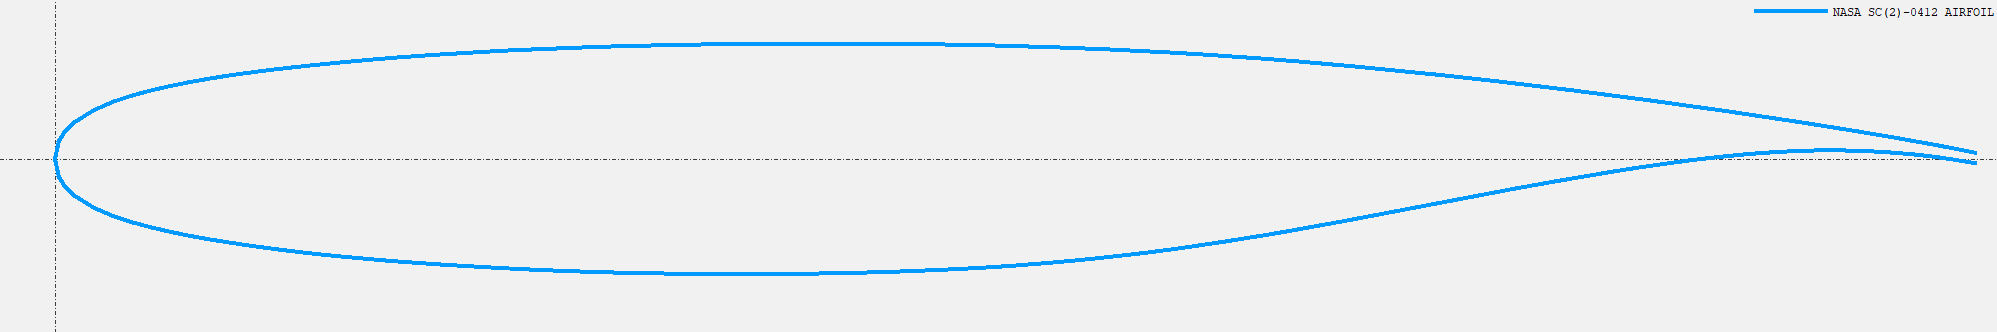
\includegraphics[width=\textwidth]{Photos/aero/sc0412.png}
    \caption{NASA SC(2)-0412 Airfoil Cross-Section}
    \label{fig:0412airfoil}
\end{figure}
\begin{figure}[!h]
    \centering
    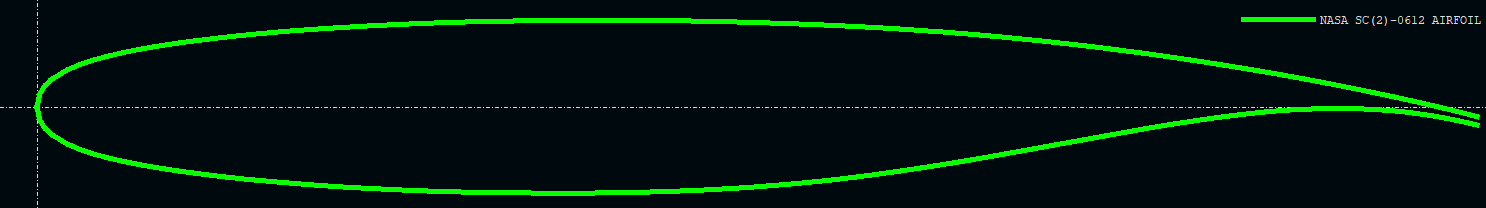
\includegraphics[width=\textwidth]{Photos/aero/sc0612.png}
    \caption{NASA SC(2)-0612 Airfoil Cross-Section}
    \label{fig:0612airfoil}
\end{figure}
\begin{figure}[!h]
    \centering
    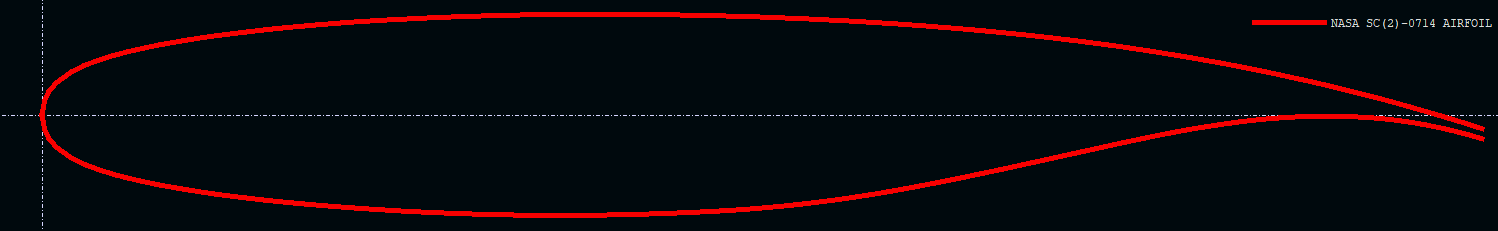
\includegraphics[width=\textwidth]{Photos/aero/sc0712.png}
    \caption{NASA SC(2)-0712 Airfoil Cross-Section}
    \label{fig:0712airfoil}
\end{figure}
\clearpage
\begin{figure}[!h]
    \centering
    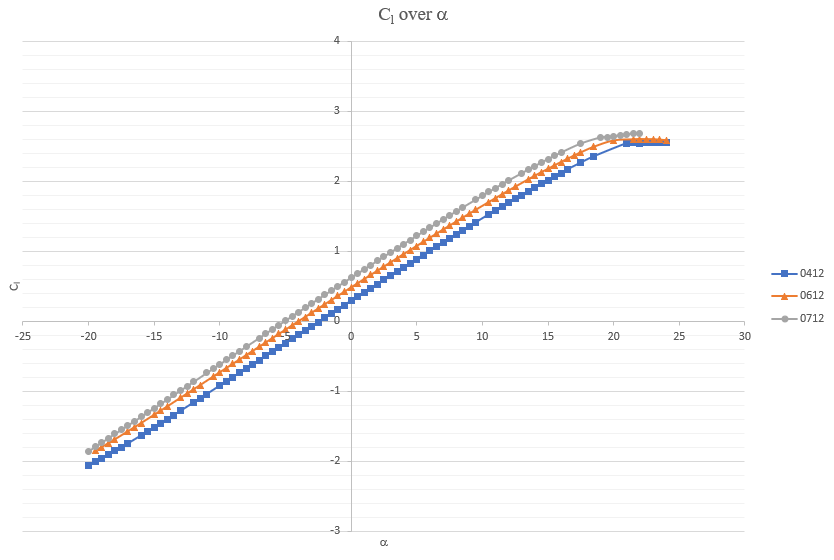
\includegraphics[width=\textwidth]{Photos/aero/AirfoilAnalysis.png}
    \caption{Airfoil $C_L$ vs $\alpha$ Comparison}
    \label{fig:airfoils}
\end{figure}

As shown above in the graphical analysis of the $C_L$ vs $\alpha$ polar, Figure \ref{fig:airfoils}, a favorable increase in lift coefficient results from SC(2)-0712.  Due to the mission requirement of serving as a high-capacity, medium-range aircraft, it is proposed to use the NASA SC(2)-0412 supercritical airfoil.  While the SC(2)-0714 airfoil presented favorable lift coefficients, the SC(2)-0412 resulted in a higher stall angle of attack with a minimal penalty difference of $\Delta C_L = -0.1392$.  The SC(2)-0412 airfoil is continuous for the entire span of its wing.  Aerodynamic twist is not introduced for fabrication efficiency and cost saving.  Later analyses in Section \ref{sec:highlift} observe the impacts of high lift devices such as Fowler Flaps and leading edge slats.


\newpage
\subsection{Wing Design}
Initial assumptions were made for the aspect ratio of the wing design based on comparable aircraft such as the Boeing 777-200 and Boeing 787.  Consequently, a range of AR $ \in [8,12]$ was initially set.  A wing area of $5,000 \text{ ft}^2$ was recommended from the initial performance analysis.  More detailed contour analysis proved better range performance and weight saving with a wing reference area of $4,000 \text{ ft}^2$, as shown in Figure \ref{fig:contourf}.

\begin{figure}[!h]
    \centering
    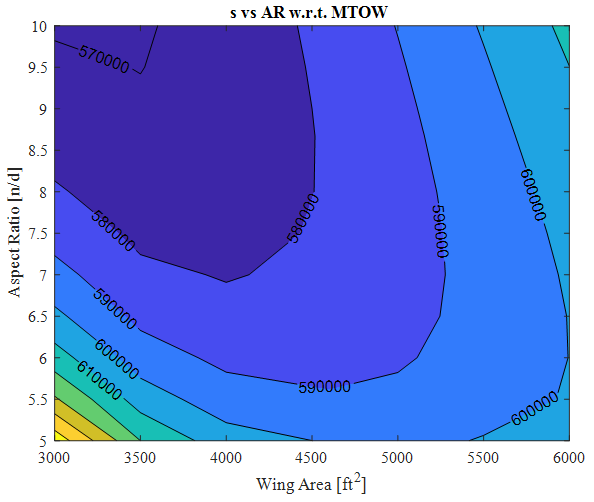
\includegraphics[width=0.85\textwidth]{Photos/aero/ARWingcontourf.png}
    \caption{Contour Plot for AR vs Wing Area}
    \label{fig:contourf}
\end{figure}

The modified wing dimensions are shown to the below in Table \ref{tab:wingsizing}.  The modified values provided a much more realistic wing span for the requirements.  Next steps involve generating the wing geometry in XFLR5 to determine aerodynamic characteristics.  The entire span of the wing uses the SC(2)-0412 airfoil with a dihedral angle of $2.5\degree$ and angle of incidence of $2.5 \degree$.  The angle of incidence improved the take-off and landing performance by increasing the coefficient of lift with minimal drag penalty.  Further studies into the effects of dihedral angle on the stability of the aircraft will be discussed in Section \ref{section: Stab and Control}.


\begin{figure}[!h]
    \centering
    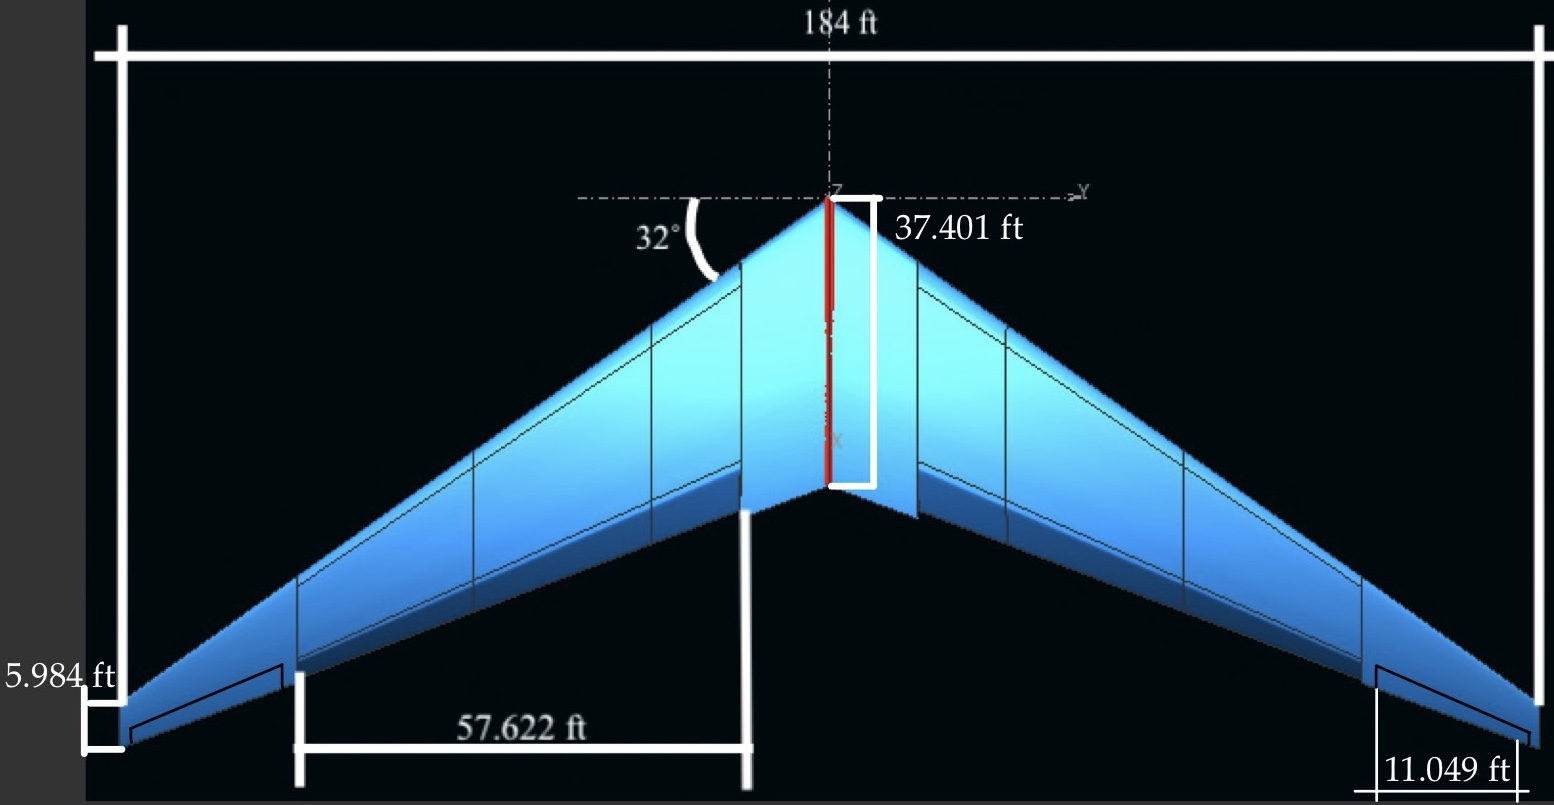
\includegraphics[width=0.95\textwidth]{Photos/aero/wing_flapped.png}
    \caption{Wing Dimension with Flaps and Slats}
    \label{fig:winged}
\end{figure}

\begin{table}[!h]
    \centering
    \caption{Wing Dimensions}
    \begin{tabular}{|c|c|c|c|} \toprule
        \multicolumn{4}{c}{\textbf{\textcolor{cobalt}{Main Wing}}} \\ \midrule
        \textbf{Description} & \textbf{Initial \#} & \textbf{Finalized \#} & \textbf{Units} \\ \hline \hline
        AR & 9.0 & 8.5 & $\sim$ \\ \hline
        b (\textit{span}) & 212 & 184 & ft \\ \hline 
        $s_{\text{wing}}$ (\textit{area}) & 5,000 & 4,000 & ft$^2$ \\ \hline
        c/4 Sweep & 30 & $32$ & degree \\ \hline
        $\alpha_i$ & 0 & $2.5$ & degree \\ \hline
        $+\Gamma$ (\textit{dihedral}) & 0 & $2.5$ & degree \\ \hline
        $\lambda$ & 0.18 & 0.16 & $\sim$ \\ \hline
        Chord Root & 479.39 & 452.72 & in \\ \hline
        Chord Tip & 86.29 & 67.91 & in \\ \hline   
        Mean Aerodynamic Chord & 328.37 & 307.72 & in \\ \bottomrule
    \end{tabular}
    \label{tab:wingsizing}
\end{table}
\clearpage

\subsection{High-Lift Systems}\label{sec:highlift}
High-lift devices are implemented on SAM Mark I to improve aircraft stability during take-off and landing segments of the mission profile.  Leading edge slats and trailing edge Fowler flaps are included on the wing.  The analysis for high-lift devices included five different configurations, as tabulated below in Table \ref{tab:highlyfttest}.  Due to XFLR5's limitations, take-off condition is assumed for $V_{TR} = 281.2$ ft/s.

\begin{table}[!h]
    \centering
    \caption{Analysis of High-Lifting Devices}
    \begin{tabular}{|p{1in}|p{1in}|p{0.5\textwidth}|}\toprule
        \multicolumn{1}{c}{\textbf{Configuration}} & \multicolumn{1}{c}{\textbf{Graphical Color}}& \multicolumn{1}{c}{\textbf{Description}} \\\midrule
        Flaps 0 & Cyan & $\delta_F=0\degree$ and no slats \\ \hline
        Flaps 1 & Magenta & $\delta_F = 10\degree$ and full slats \\ \hline
        Flaps 2 & Red & $\delta_F = 20\degree$ and full slats \\\hline
        Flaps 3 & Orange & $\delta_F = 30\degree$ and full slats \\\hline
        Slat Test & Green & $\delta_F = 30\degree$ with No Slats \\ \bottomrule
    \end{tabular}
    \label{tab:highlyfttest}
\end{table}

\begin{figure}[!h]
    \centering
    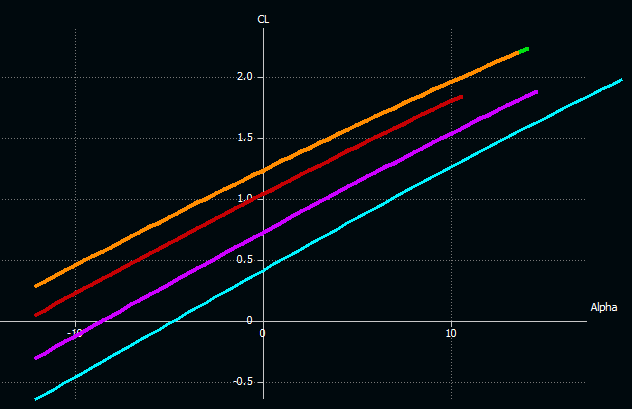
\includegraphics[width=0.8\textwidth]{Photos/aero/CL_o_alpha.png}
    \caption{$C_L$ vs. $\alpha$ for varying $\delta_F$}
    \label{fig:clalphahigh}
\end{figure}
According to Figure \ref{fig:clalphahigh}, Flap setting three provides optimal lift coefficient and is recommended for a full flaps take-off configuration.  Further analysis will determine whether Flaps 3 is also an appropriate setting for landing.  Figure \ref{fig:clcdalphahigh} displays the significant increase in drag with an increase of flap deflection.  As a result, Flap setting zero is recommended for cruise to optimize aerodynamic performance.  Additionally, the studies show smoother and steadier polars for flap conditions combined with slats.  Therefore, a recommendation of combining slats and flaps is made for SAM Mk I.

\begin{figure}[!h]
    \centering
    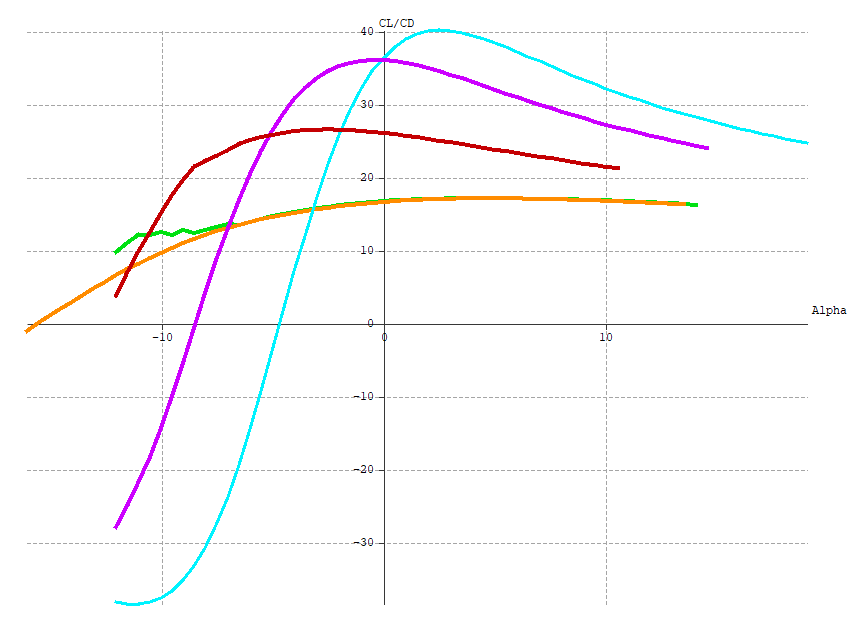
\includegraphics[width=0.8\textwidth]{Photos/aero/CL_CD_o_alpha.png}
    \caption{$\frac{C_L}{C_D}$ vs $\alpha$ for varying $\delta_F$}
    \label{fig:clcdalphahigh}
\end{figure}

\begin{figure}[!h]
    \centering
    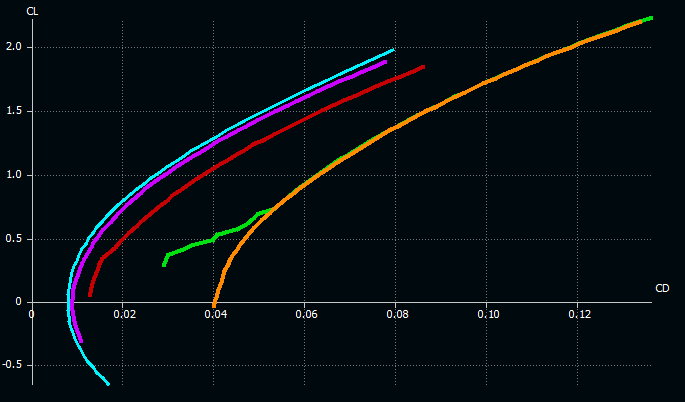
\includegraphics[width=0.8\textwidth]{Photos/aero/CL_o_CD.png}
    \caption{$C_L$ vs $C_D$ for varying $\delta_F$}
    \label{fig:clcdhigh}
\end{figure}

\begin{figure}[!h]
    \centering
    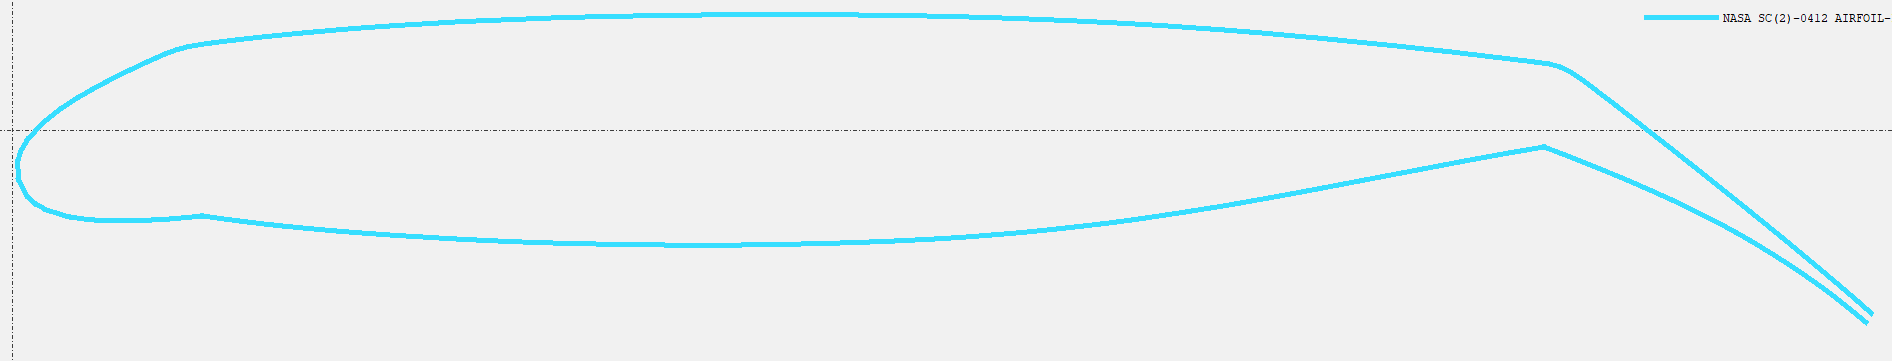
\includegraphics[width=\textwidth]{Photos/aero/sc0412flapped.png}
    \caption{SC(2)-0412 Airfoil with $\delta_F = 30\degree$ and slats}
    \label{fig:highlift}
\end{figure}

\clearpage
\subsection{Drag Buildup}
The Drag for SAM Mark I is built up part-by-part by separating the fuselage, wings, empennage, and other protuberances and calculating the following seven key forms of drag, shown in Equation \ref{eqn:drag_general} from Raymer \cite{raymer}:
\begin{equation}\label{eqn:drag_general}
    C_D = C_{D,0} + C_{D,i} + C_{D,W_{NL}} + C_{D,W_{L}} + C_{D_{EXCR}} + \Delta C_{D_{Re}} + C_{D,trim}
\end{equation}


% \subsubsection{Take-Off Drag}


% \subsubsection{Cruise Drag}
To properly predict and quantify the wave drag for aerodynamic analysis on the airfoil and wing design, two methods are tested: \textit{Method B} from Vargas \cite{vargas} and \textit{Delta Method} from Feagin \cite{deltaMethod}.  The Delta method relies on a combination of graphical comparison offsetting the McDevitt method \cite{mcdevitt} by adding the Torenbeek method \cite{torenbeek} to account for the transonic flow characteristics.  Through a graphical approach and MATLAB computed analysis, the Cruise Drag buildup is displayed in Table \ref{tab:dragbuildup}.

\begin{table}[!h]
    \centering
    \caption{Tabulated Drag Buildup}
    \begin{tabular}{|p{0.75in}|p{0.75in}|p{0.75in}|p{0.75in}|p{0.75in}|p{0.75in}|}\toprule
        \textbf{Description} & \textbf{Wing} & \textbf{Vertical \newline Stabilizer} & \textbf{Horizontal \newline Stabilizer} & \textbf{Fuselage} & \textbf{Nacelle}  \\ \midrule
        $S_{wet} (ft^2)$ & 8,095 & 1,012 & 2024 & 11,384 & 1,194 \\ \hline
        Reynolds Number & $4.77x10^7$ & $3.68x10^7$ & $3.01x10^7$ & $4.36 x 10^8$ & $5.46 x 10^7$ \\ \hline
        $C_{f}$ & $2.306 x 10^{-3}$ & $2.388 x 10^{-3}$ & $2.455 x 10^{-3}$ & $1.596 x 10^{-3}$ & $2.163 x 10^{-3}$ \\ \hline
        $FF$ & $1.570$ & $1.3500$ & $1.3500$ & $1.046$ & $1.184$ \\ \hline
        \textbf{$(C_{D_{0}})_{cruise}$} & $6.196 x 10^{-3}$ & $7.700 x 10^{-4}$ & $1.583 x 10^{-3}$ & $4.486 x 10^{-3}$ & $7.217x10^{-4}$ \\ \midrule
        \textbf{$C_{D,W}$} & $3.214 x 10^{-3}$ & $\sim$ & $\sim$ & 0 & $\sim$ \\ \hline
        
    \end{tabular}
    \label{tab:dragbuildup}
\end{table}

In calculating the total parasitic drag, $C_{D_{0}}$ of SAM Mk I, an additional two to five percent increase in drag accounts for the leakage and protuberance drag. \cite{raymer}  Using a part-by-part analysis and including the Delta method to account for wave drag, the estimated total coefficient of drag during cruise is $3.211 x 10^{-2}$.




\subsection{Future Progress}
Several key topics are under active investigation to improve the aircraft performance. The following will be further investigated for the Preliminary Design Report:
\begin{itemize}
    \item Confirm Drag Coefficients for take-off and landing analysis
    \item Investigate use of Flaperons for cruise roll stability
    \item CFD analysis of complete wing and body system
\end{itemize}


% \textcolor{red}{
% \begin{itemize}
%     \item Discuss airfoil selection, including reasoning, lift curves, drag polar.
%     \begin{itemize}
%         \item Selection should not solely be from using XFOIL!
%         \item Airfoil selection should encompass multiple methods
%     \end{itemize}
%     \item Discuss wing design, including reasoning, geometry, and CAD drawings with dimensions
%     \begin{itemize}
%         \item Label diagram and tabulate important parameters.
%     \end{itemize}
%     \item CAD is expected for major drawings
%     \item Discuss high-lift system, including reasoning, geometry, and CAD drawings with dimensions
%     \item Discuss drag buildup (tabulated), including cruise, takeoff, and landing
%     \begin{itemize}
%         \item Describe your methods and include significant contributions
%     \end{itemize}
%     \item Discuss aircraft lift curves and drag polars, including cruise, takeoff, and landing.
%     \begin{itemize}
%         \item Identify key mission points on these plots.
%         \item Describe methods and limitations.
%     \end{itemize}
%     \item Summarize key aircraft information (tabulated) at cruise, takeoff, and landing (e.g. angle of attack, lift coefficient, drag coefficient).
%     \item Include at least two trade studies that use quantitative analysis to support design decisions made.
%     \begin{itemize}
%         \item One should be airfoil selection
%         \item Describe system-level tradeoffs (if any)
%     \end{itemize}
%     \item Discuss parachute sizing if required.
%     \item Discuss future work.
%     \item \hl{Important aerodynamic characteristics and aerodynamic performance for key mission segments and requirements AERO or PERF}
% \end{itemize}}

\clearpage
\section{Performance (\textit{MK})}
\label{section: Performance}
\subsection{Mandatory Performance (\textit{JJ, MK})}
\label{mand}
The AIAA RFP \cite{RFP} requires this short range aircraft to have a range of 3,500 NM with the ability to carry a capacity of 400 passengers in a dual class configuration. The aircraft must also have enough reserves to fly to an alternate airport 200 NM from the destination airport, hold for 30 minutes at the alternate airport, and contain 5\% contingency fuel, which is defined as 5\% of non-reserve block fuel. Furthermore, both takeoff and landing distances are restrained to 9,000 ft or less off asphalt or concrete runways at International Standard Atmosphere (ISA) +15 degrees Celsius conditions. Finally, the maximum approach speed the aircraft can have is 145 knots calibrated airspeed (KCAS) at the end of the design mission. 

% \subsection{Predicted Performance (\textit{MK})}
% First-cut analysis was performed using an estimated empty weight as well as a fuel weight calculated by using a thrust-specific fuel consumption (TSFC) average of contemporary large turbofan engines, such as what would be found on an aircraft of this size.  This data was then input into a time-step integration spreadsheet to converge on a first design for a bounded range for cruise. For the duration of cruise, the aircraft will begin cruising at an altitude of FL370, where it will perform two step climbs of 3000 ft each and end at a cruising altitude of FL430. Before and after cruise, the aircraft will follow the mission profile as stated in Section \ref{section: Conops} in Figure \ref{fig:missionprof}.

% In the future, the flight envelope as well as fuel estimation of each segment in the mission profile will be performed. Additionally, the time-step integration of cruise will be refined and the time-step integration process will be implemented for the climb, descend, and loiter segments of the mission. Further analysis will performed on determining the drag of each mission segment as well as regulating that the design stays within the requirements set forth by the RFP \cite{RFP}. obsolete now

\subsection{Determination of Cruising Altitude (\textit{MK})}
To determine a valid cruising altitude, a trade study was performed on the two-class capacity of similiar aircraft that either are currently in service or were in the past. This will facilitate the decision of which altitude will be best to cruise at for SAM Mk 1. Figure \ref{cruxalt} shows four aircraft and their respective cruising altitudes and two-class passenger capacity\cite{butterworth}.

\begin{table}[!h]
    \centering
        \caption{Cruise Altitude Comparison of Similar Capacity Aircraft}
    \begin{tabular}{|c||c|c|c|c|}\toprule
         & \textbf{B747-200} & \textbf{B777-200} & \textbf{A340-600} & \textbf{IL96-M}\\ \hline \hline
         \textbf{Manufacturer} & Boeing & Boeing & Airbus & Ilyushin \\ \hline
         \textbf{Cruise Altitude [ft]} &  35,000 & 39,000 & 41,000 & 30,000 \\ \hline
         \textbf{2-Class Capacity} & 442 & 375 & 440 & 335\\ \bottomrule
    \end{tabular}
    \label{cruxalt}
\end{table}

From the trade study, it can be seen that all the aircraft listed range in cruising altitudes from 35,000 ft to 41,000 ft. The next step was taken the average of each aircraft's cruising altitude and passenger capacity. The average cruising altitude between the aircraft is 36,500 ft, while the average passenger capacity is 398 passengers. From these averages, similar capacity aircraft tend to cruise at an altitude just above the tropopause. Thus, from analysis, Team Toucan has decided to design SAM Mk. I to cruise at an altitude of 37,000 ft.

\subsection{Determination of Cruise Speed}
\label{crusspeed}
\subsubsection{Trade Study of Commercial Aircraft Cruise Speeds (JJ)}
A trade study of common turbine-powered commercial aircraft ranging in size and age from both Boeing and Airbus was performed on the basis of determining their respective cruise speed and maximum fuel range (as reported by manufacturer).  All data used in this trade study came from one source:  \cite{butterworth}, with the cruise speed converted from velocity to Mach number at the specified cruise altitude respective to each plane. 

\begin{table}[!h]
    \centering
        \caption{Comparison of Cruise Speed for Turbine-Powered Aircraft}
    \begin{tabular}{|p{1.1in}||c|c|c|c|c|c|c|}\toprule
         & \textbf{B747-400} & \textbf{B757-200} & \textbf{B767-400} & \textbf{B777-200} & \textbf{A320-200} & \textbf{A330-300} & \textbf{A340-600} \\\hline \hline
         \textbf{Manufacturer} & Boeing & Boeing & Boeing & Boeing & Airbus & Airbus & Airbus\\ \hline
         \textbf{Cruise Mach} & 0.85 & 0.80 & 0.80 & 0.75 & 0.74 & 0.76 & 0.82\\ \hline
         \textbf{Max. Range [NM]} & 7260 & 4488 & 5625 & 4820 & 3672 & 7046 & 7800 \\ \bottomrule
    \end{tabular}
    \label{tab:cruisecomp}
\end{table}

\newpage
This information leads to a mean cruise speed (of these selected planes) equal to Mach 0.788.  This study was performed to augment the analytical determination, \ref{cruisespeed}, as factors such as time of flight and airline (operator) preference also play a role in determining a desirable cruise speed.

\subsubsection{Analytical Determination of Cruise Speed (\textit{MK})} \label{cruisespeed}
It is established that best aerodynamic performance during steady, level flight (cruise) corresponds to the same maximum range speed as the occurrence of $(\frac{C_{L}^{1/2}}{C_{D}})_{max}$, which corresponds to the minimum power required. This can be found analytically by plotting total drag on a thrust required versus velocity chart. Then, the local minimum corresponds to $(\frac{C_{L}^{1/2}}{C_{D}})_{max}$, which then indicates the optimal Mach number. Figure \ref{optimach} visually demonstrates this theory, and shows the optimal Mach number to be 0.996 at a $(\frac{C_{L}^{1/2}}{C_{D}})_{max}$ of 23.9. 

Now, comparing the analytical method to the trade study, the values vary by quite a bit. However, the Mach number determined through the analytical method is much higher than what aircraft of this type and size usually have. This could be due to the plot underestimating the amount of drag. Thus, for the remainder of the project, Team Toucans decided to choose a Mach number to be slightly less than the trade study Mach number, with a greater weight applied towards the Mach number determined from trade study. The final cruise Mach number was chosen to be Mach 0.775.

\begin{figure}[H]
    \centering
    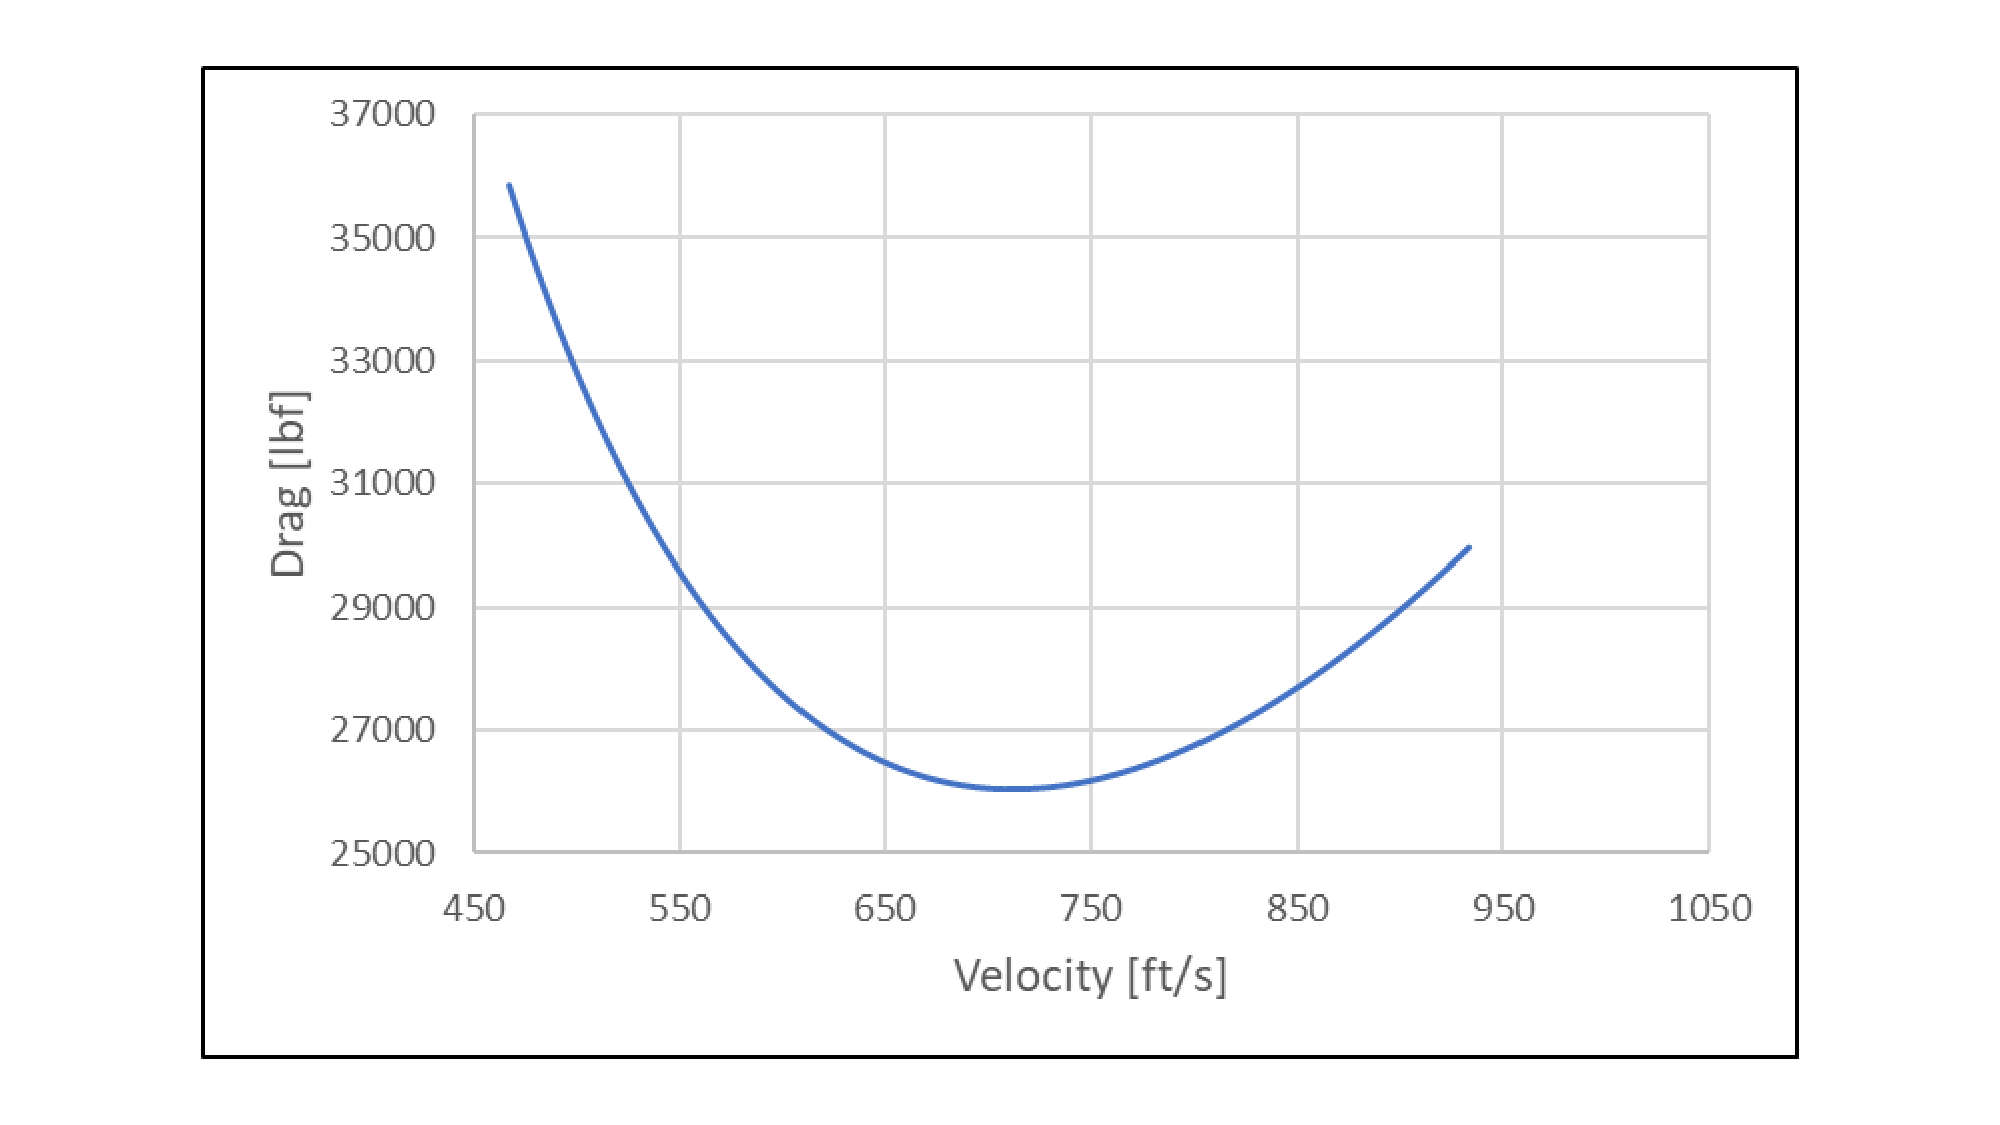
\includegraphics[width=1.0\textwidth]{Photos/Optimal_Mach.pdf}
    \caption{Optimal Mach Number at \boldmath{$(\frac{C_{L}^{1/2}}{C_{D}})_{max}$}}
    \label{optimach}
 \end{figure}

\subsection{Takeoff and Landing Analysis (\textit{MK})}
\qquad
When analyzing takeoff and landing distances, Team Toucan used the methods described in Raymer \cite{raymer} Chapter 17 and accounted for multiple runway conditions. Specifically, the ground roll, rotation, transition and climb distances for take-off along with the approach, flare and ground distances for landing are shown in Table \ref{tab:TO} and Table \ref{tab:land}, respectively. The takeoff distances were calculated assuming OEI, which follows the certification CFR Part 25.107 \cite{cfr}.

\begin{table}[!h]
    \centering
    \caption{Takeoff Distance - Each Segment}
    \begin{tabular}{|>{\centering}p{1.1in}|>{\centering}p{.3in}|>{\centering}p{1.0in}|>{\centering}p{.75in}|>{\centering}p{.83in}|>{\centering}p{.6in}|>{\centering\arraybackslash}p{.6in}|}\toprule 
    \textbf{Runway Condition} & \boldmath{$\mu$} \textbf{\cite{raymer}} & \textbf{Ground Roll [ft]} & \textbf{Rotation [ft]} & \textbf{Transition [ft]} & \textbf{Climb [ft]} & \textbf{TOFL [ft]} \\ \hline \hline
    Dry Concrete & 0.03 & 4,540 & 820 & 760 & 210 & 6,330 \\ \hline
    Wet Concrete & 0.05 & 4,660 & 820 & 760 & 210 & 6,450\\ \hline
    Wet Grass & 0.08 & 4,880 & 820 & 760 & 210 & 6,670\\ \hline
    Firm Dirt & 0.04 & 4,600 & 820 & 760 & 210 & 6,390 \\ \bottomrule
    \end{tabular}
    \label{tab:TO}
\end{table}
\clearpage 

\begin{table}[!h]
    \centering
    \caption{Landing Distance - Each Segment}
    \begin{tabular}{|p{1.1in}|p{.3in}|p{.8in}|p{.6in}|p{1.0in}|p{.55in}|}\toprule 
    \textbf{Runway Condition} & \boldmath{$\mu$} \textbf{\cite{raymer}} & \textbf{Approach [ft]} & \textbf{Flare [ft]} & \textbf{Ground Roll [ft]} & \textbf{LFL [ft]} \\ \hline \hline
    Dry Concrete & 0.3 & 1,530 & 210 & 3,700 & 5,440  \\ \hline
    Wet Concrete & 0.15 & 1,530 & 210 & 7,640 & 9,380\\ \hline
    Wet Grass & 0.2 & 1,530 & 210 & 5,640 & 7,380\\ \hline
    Hard Turf & 0.4 & 1,530 & 210 & 2,760 & 4,500\\ \bottomrule
    \end{tabular}
    \label{tab:land}
\end{table}

Moreover, during the landing phase of the mission, the maximum landing weight of the aircraft was determined to be 395,000 lb, which gives the SAM Mk. I a max landing weight fraction of about 0.878. The aircraft will also takeoff with a velocity of approximately 160 KTAS. and will land with a maximum velocity of 145 KCAS, as stated in the RFP. The results described in Figure \ref{tab:land} assume the aircraft burned all non-block fuel required for the design mission. Finally, from the estimates, excluding wet concrete, SAM Mk I meets the requirements set forth by the RFP. This gives the SAM Mk I the capability to operate in a wide range of airports with runways longer than 6,400 ft on dry concrete for takeoff and runways longer than 5,500 ft on dry concrete for landing.

\subsection{Rate of Climb (\textit{MK})}
After takeoff, SAM Mk I will begin to perform the climb process. The aircraft will start to climb immediately after take-off and climb to the first cruising altitude of 37,000 ft. By using a time-step integration, Team Toucan obtained an estimated rate of climb of 7,100 ft/min, with a flight path angle of about 16 degrees. In these estimations, both engines were included, but were not at full thrust capacity for the duration of climb. Instead, the time-step integration method assumed the engines operation at 70\% thrust. Additionally, the total fuel consumed during the climb segment of the mission was estimated to be about 8,060 lb, with a total climb time of slightly less than 13 minutes, also using the time-step integration method described earlier. Finally, it was estimated that through the duration of the process, the aircraft will have traveled about 145 NM in the horizontal distance.

The service ceiling of the aircraft was determined by further analyzing rate of climb in a time-step integration method. Specifically, the service ceiling is defined when the aircraft achieves a rate of climb of less than 500 ft/min. To visually inspect this, a plot of rate of climb as a function of altitude can be used. The service ceiling of SAM Mk 1, shown by the dotted line in Figure \ref{serceil}, is about 46,500 ft. One note about this service ceiling is that this was determined with both engines running at maximum thrust capacity.  

\begin{figure}[H]
    \centering
    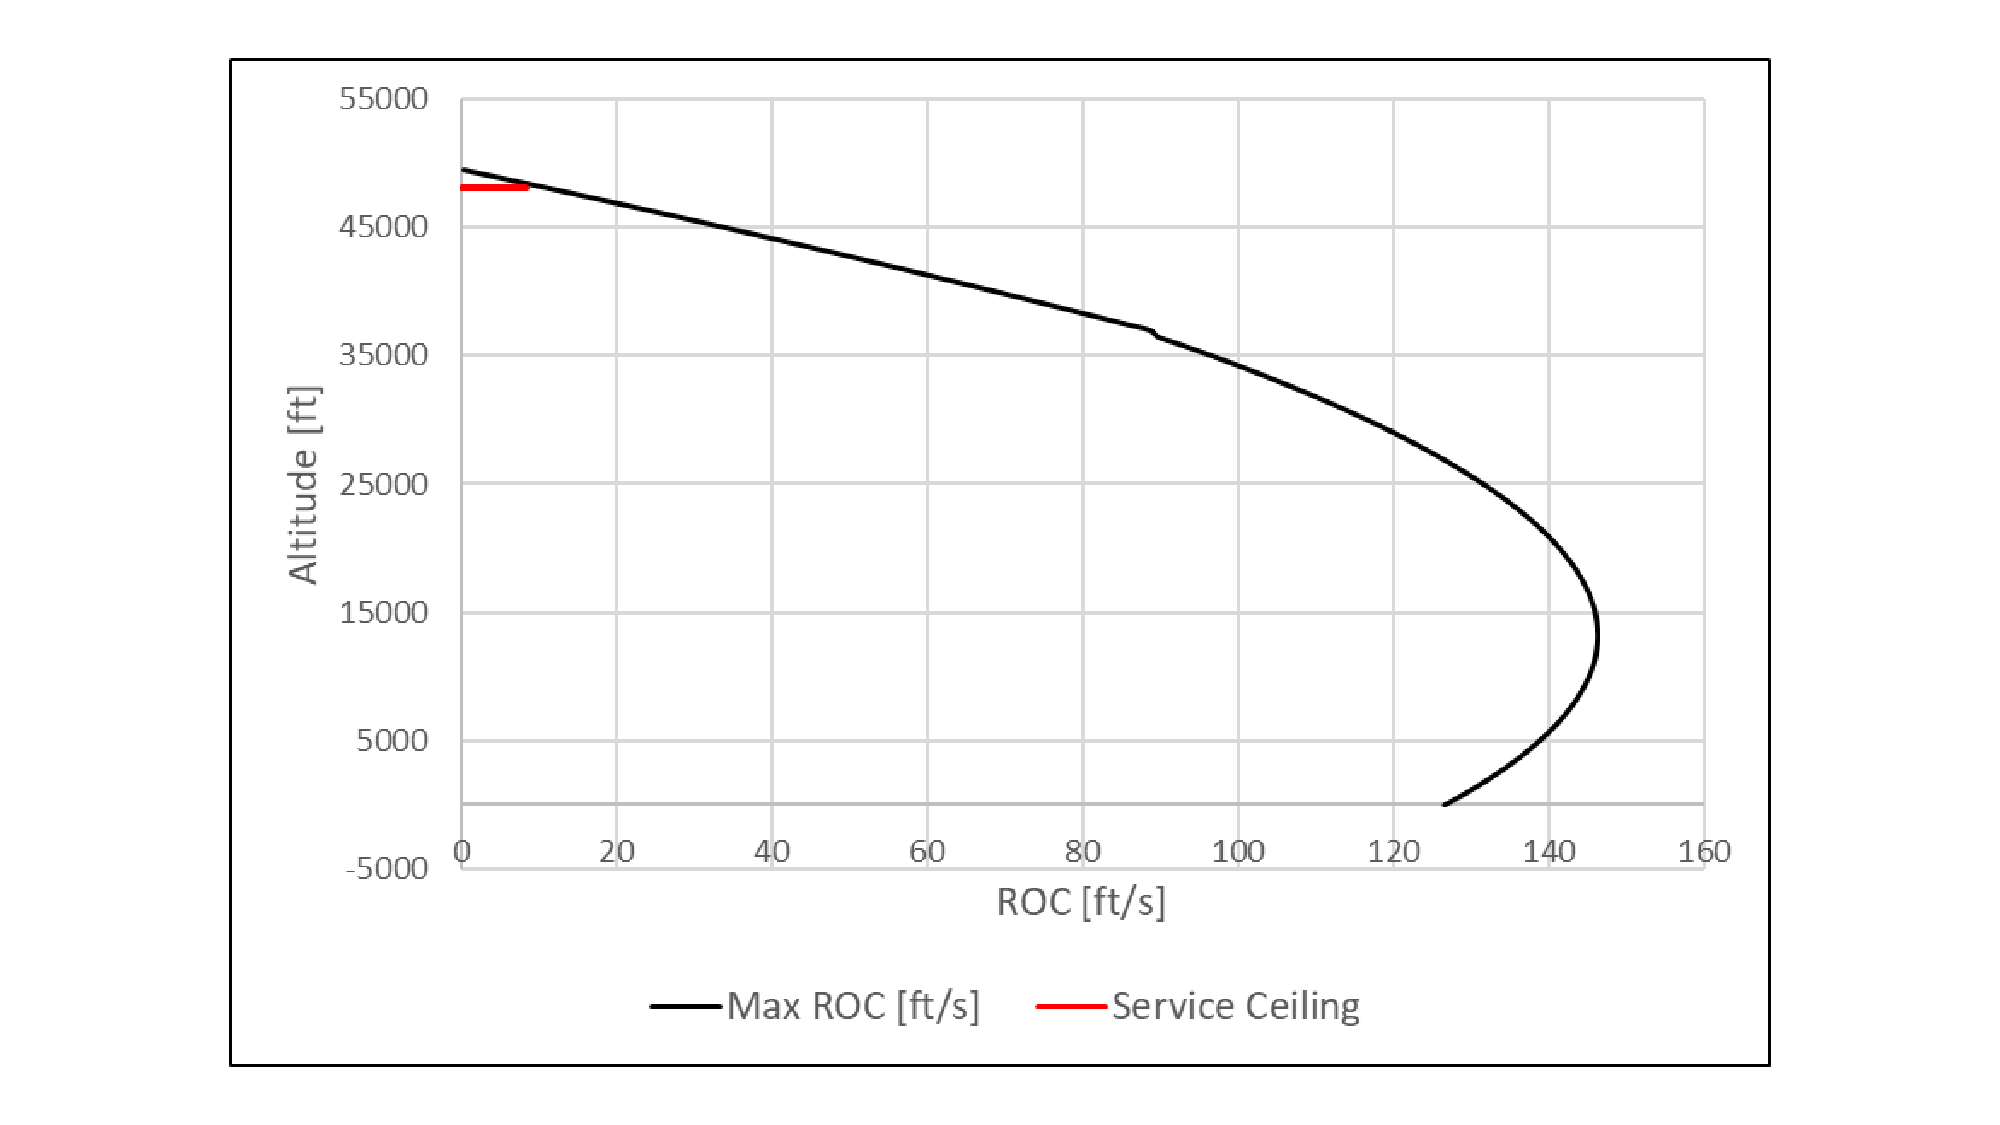
\includegraphics[width=1.0\textwidth]{Photos/Service_Ceiling.pdf}
    \caption{Service Ceiling -  SAM Mk 1}
    \label{serceil}
 \end{figure}

\subsection{Cruise (\textit{MK})}
An important part of the of the mission of the SAM Mk I is the cruise segment. In this segment, the design cruise speed was chosen to be M 0.775, as described in Section \ref{crusspeed}. Next, the aircraft will begin the cruise segment at an altitude of 37,000 ft, where it will step climb in segments of 2,000 ft to 39,000 ft and 41,000 ft, respectively. This process is performed to maintain a constant and high lift-to-drag ratio throughout the cruise segment of the design mission. Two methods were used to estimated the overall performance of the cruise segment. First, a time-step integration was used to determine the range and endurance of our aircraft. Each step climb was performed after a third of the allotted cruise fuel (which will be discussed in Section "Fuel per Mission Segment") was burned during the process. Once the allotted cruise fuel was all burned, the total range and total endurance of the aircraft was calculated. Second, the total range and total endurance were calculated using the Breguet-Range and Breguet-Endurance equations. This was then compared to the time-step integration method to determine the accuracy of both methods to one another. Table \ref{tab:cruise} shows the range, endurance, and percent error between both methods. 

\begin{table}[!h]
    \centering
    \caption{Cruise: Breguet Method and Time-step Integration}
    \begin{tabular}{|p{1in}||p{1in}|p{1.5in}|p{1in}|}\toprule 
     & \textbf{Breguet Method} & \textbf{Time-step Integration} & \textbf{\% Difference} \\ \hline \hline
    \textbf{Range [NM]} & 3,500 & 3,504 & 0.11 \\ \hline
    \textbf{Endurance [hr]} & 7.76 & 7.77 & 0.11 \\ 
    \bottomrule
    \end{tabular}
    \label{tab:cruise}
\end{table}

From the data, SAM Mk I successfully meets the range requirement set by the RFP. Additionally, it can be seen that the difference between the Breguet method and time-step integration is quite small, thus, solidifying the use of the Breguet method for cruise estimation. 

\subsection{Fuel per Mission Segment (\textit{MK})}
An important parameter to determine for SAM Mk I is how much fuel is required for the duration of the mission. The mission can be broken up into two main section: non-block and reserves. In the non-block section, the segments include Warm-up, Taxi, and TO (WUTTO), Climb, Cruise, Descend, 5 minute loiter at 5,000 ft, and Approach, Landing, and Taxi (ALT). The reserves will contain a climb to 30,000 ft, a 200 NM alternate to another airport, a 30 min loiter at the airport, descend, 5\% contingency fuel, and a 5 minute loiter at 5,000 ft. Weight fractions from Raymer\cite{raymer} were used for WUTTO and ALT. Fuel estimation for cruise and alternate destination was determined using Breguet range while the loiter segments used Breguet Endurance equations. Finally, all climb and descend values were estimated using a time-step integration method. Table \ref{fuelfrac} shows the calculated fuel fractions. 

\begin{table}[!h]
    \centering
    \caption{Fuel Fractions for Each Mission Segment}
    \begin{tabular}{|p{1.75in}||p{1in}|p{1.5in}|}\toprule 
    \textbf{Mission Segment} & \textbf{Fuel Weight [lb]} & \textbf{Calculated Fuel Fraction}\\ \hline \hline
    WUTTO & 6,750 & 0.985 \\ \hline
    Climb & 8,060 & 0.982  \\ \hline
    Cruise & 95,950 & 0.786 \\ \hline
    Descend & 6,420 & 0.986 \\ \hline
    ALT & 1,660 & 0.996 \\ \hline
    5 min Loiter (5,000 ft) & 910 & 0.997 \\ \hline
    Climb to 30,000 ft & 4,430 & 0.990 \\
    \hline
    200 NM Alternate & 2,090 & 0.995 \\ \hline
    30 min Loiter & 7,370 & 0.984 \\ \hline
    Descend & 5,160 & 0.988 \\ \hline
    5\% Contingency Fuel & 5,990 & 0.987 \\ \hline
    5 min Loiter (5,000 ft) & 1,240 & 0.997 \\ \hline
    \textbf{Total} & \textbf{146,860} & \textbf{0.679} \\
    \bottomrule
    \end{tabular}
    \label{fuelfrac}
\end{table}

\subsection{Drag per Mission Segment (\textit{MK})}
During each segment, there is associated parasitic drag and drag due to lift. Team Toucans utilized multiple methods for different segments of the mission. Specifically, the Climb, Cruise, and Descend segments were calculated using a time-step integration, while the Takeoff and Landing Segments utilized the drag equation. Additionally, the conditions for each of the segments were set by the RFP for takeoff and landing. Due to there being variations in the drag, Table \ref{dragseg} shows drag ranges for each segment of the mission. 

\begin{table}[h]
    \centering
    \caption{Drag per Mission Segment}
    \begin{tabular}{|p{1.5in}|p{1in}|}\toprule 
    \textbf{Mission Segment} & \textbf{Drag Range [lb]} \\ \hline \hline
    Takeoff & 0-46,000 \\ \hline
    Climb & 26,000-30,500   \\ \hline
    Cruise & 25,100-26,100 \\ \hline
    Descend & 20,500-27,400 \\ \hline
    Landing & 0-14,800 \\
    \bottomrule
    \end{tabular}
    \label{dragseg}
\end{table}

\subsection{Payload-Range Diagram (\textit{MK})}
The payload-range diagram is used to analyze the range of the aircraft as payload weight is traded for fuel weight. The payload-range diagram illustrating this relationship can be seen in Figure \ref{payrang}. The lines in the diagram were calculated using the Breguet-Range method. The top line up to point A uses a payload weight of 94,300 lb and a cruise fuel weight of 95,950 lb. Then, the line from point A to point B maximizes the total fuel capacity of SAM Mk 1, which adds about 44,140 lb of fuel to the cruise fuel weight and brings the total to 140,090 lb of cruise fuel weight. Finally, the line from point B to point C represents the aircraft going to zero payload weight at the same max fuel weight from the previous line. This results in the SAM Mk 1 having a maximum range of about 6,240 NM at zero payload weight and maximum fuel weight.

\begin{figure}[H]
    \centering
    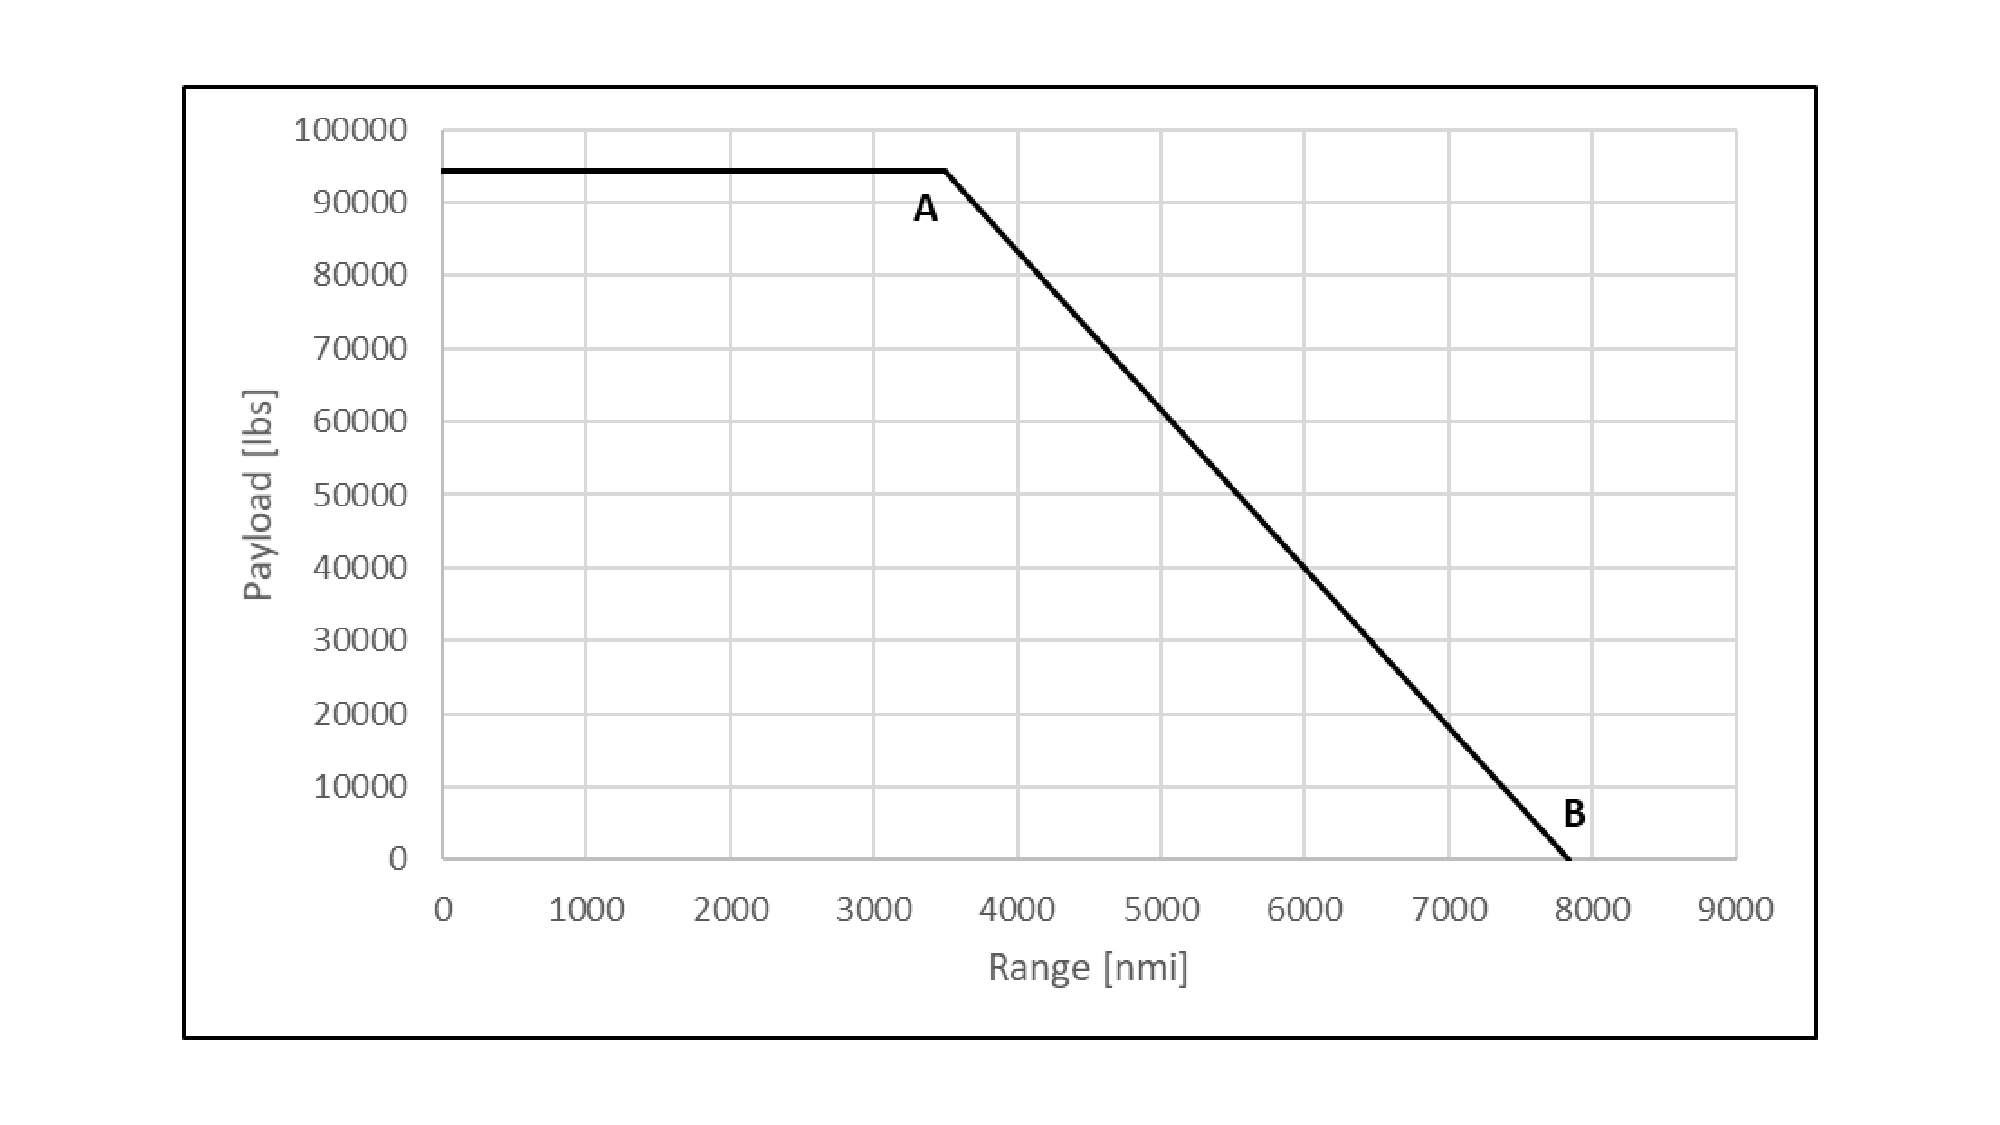
\includegraphics[width=1.0\textwidth]{Photos/Payload_Range.pdf}
    \caption{Payload-Range Diagram -  SAM Mk. I}
    \label{payrang}
 \end{figure}

\subsection{Flight Envelope (\textit{MK})}
\label{ssfl}
The flight envelope is an important diagram that demonstrates the capability of an aircraft, in terms of speed and what the altitude limits are. Additionally, it shows the service ceiling of the aircraft. For SAM Mk 1, the maximum and minimum design velocities at sea-level were determined to be 640 kts and 150 kts, respectively. The maximum velocity was determined from the max speed at which the aircraft could structurally fly (max dive speed), which will be discussed further in the Loads Section. The minimum speeds was bounded by the stall speed of the SAM Mk I. Furthermore, the absolute ceiling of SAM Mk I was determined to be 49,700 ft. This shows that SAM Mk I's cruising altitudes are within the minimum and maximum parameters. A visual representation of the flight envelope can be seen in Figure \ref{flyenv}, with the green shade corresponding to the velocity and altitude limits of the aircraft. 

\begin{figure}[!h]
    \centering
    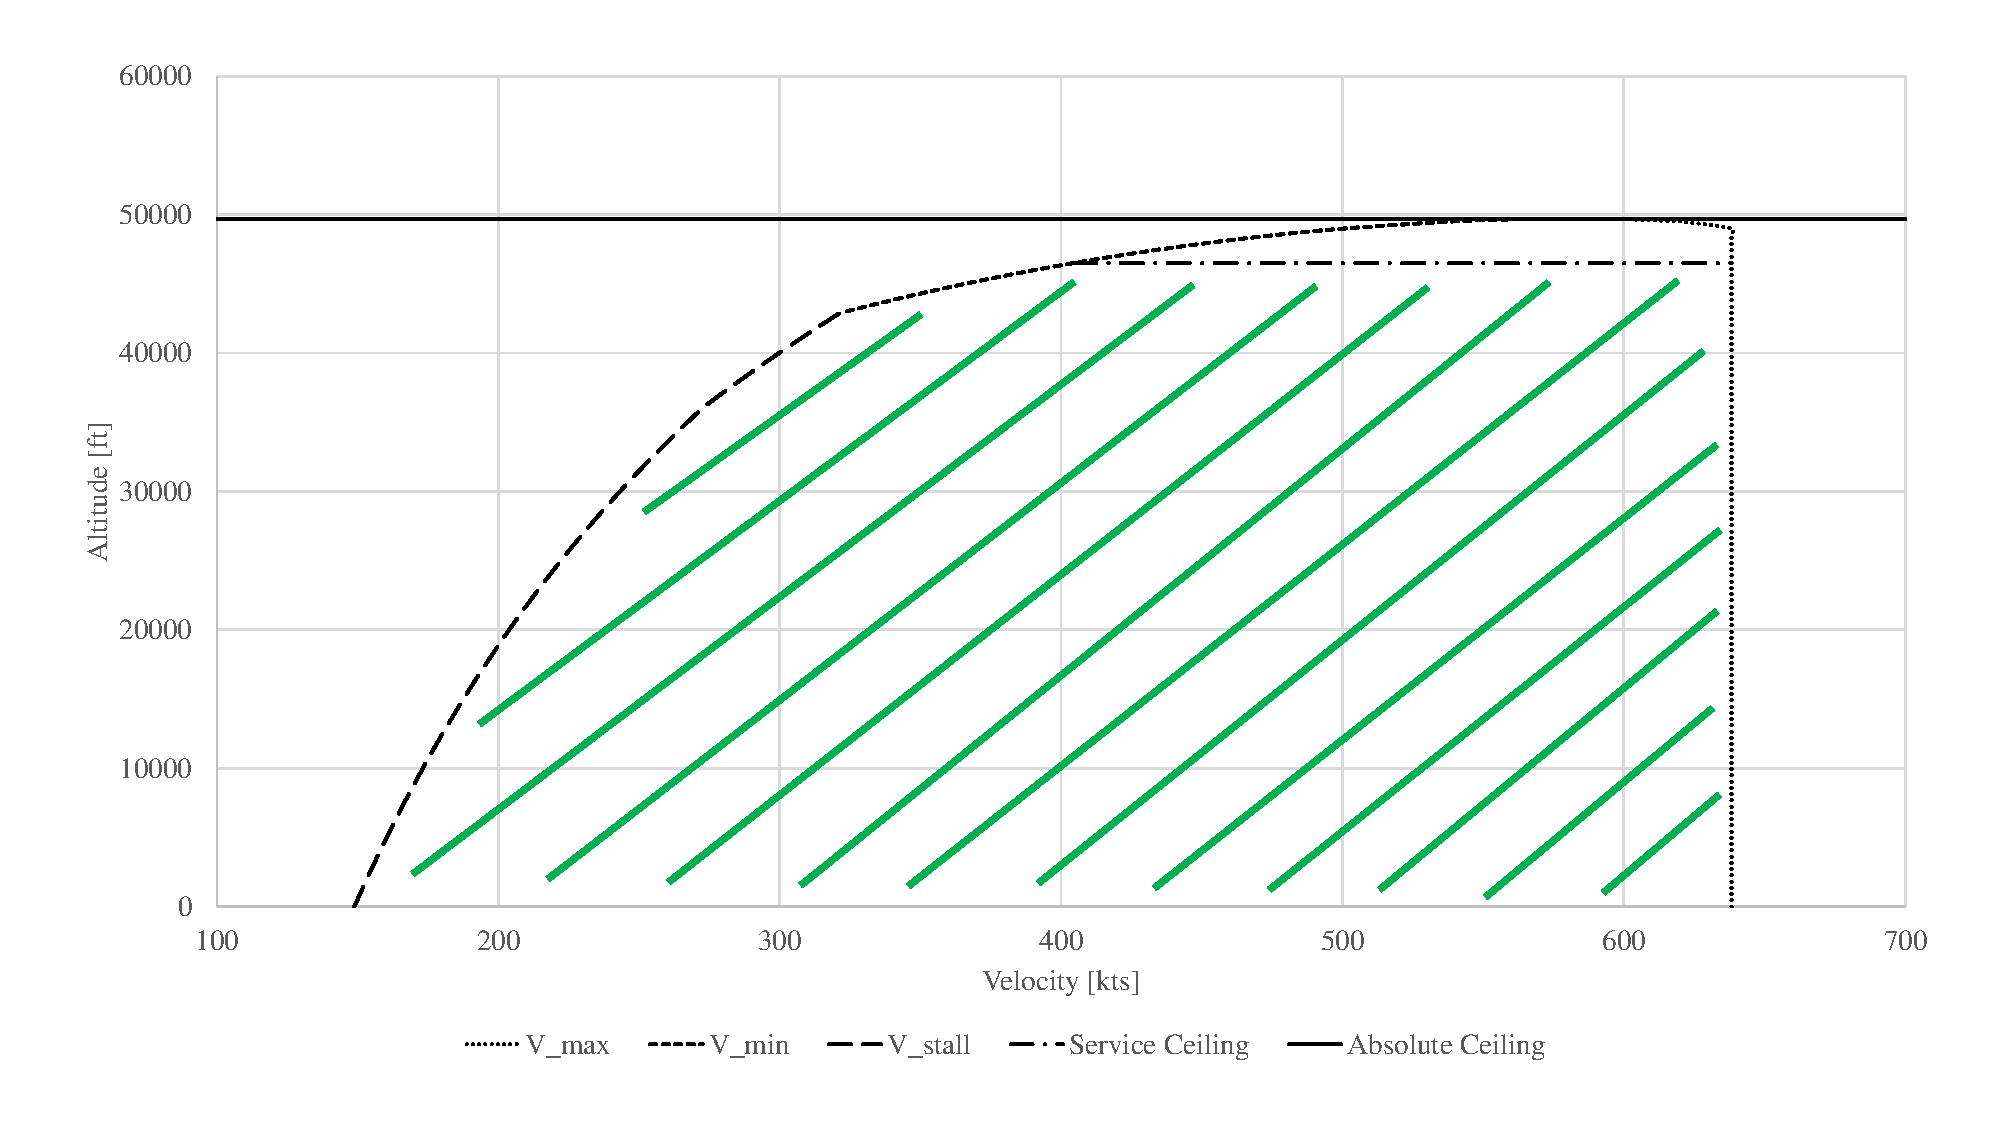
\includegraphics[width=1.0\textwidth]{Photos/Flight_Envelope.pdf}
    \caption{Flight Envelope (shaded) -  SAM Mk. I}
    \label{flyenv}
 \end{figure}
\clearpage

\subsection{Specific Excess Power Diagram (\textit{MK})}
One diagram that demonstrates the full capability of the aircraft is the Specific Excess Power, or $P_{s}$ diagram. This plot functions similarly to the flight envelope, as shown in Section \ref{ssfl}, but it does not reveal as much about the performance of the aircraft. The $P_{s}$ diagram is shown in Figure \ref{spexpw}, where specific excess power was calculated using the general specific excess power equation at varying Mach numbers and altitudes.

\begin{figure}[H]
    \centering
    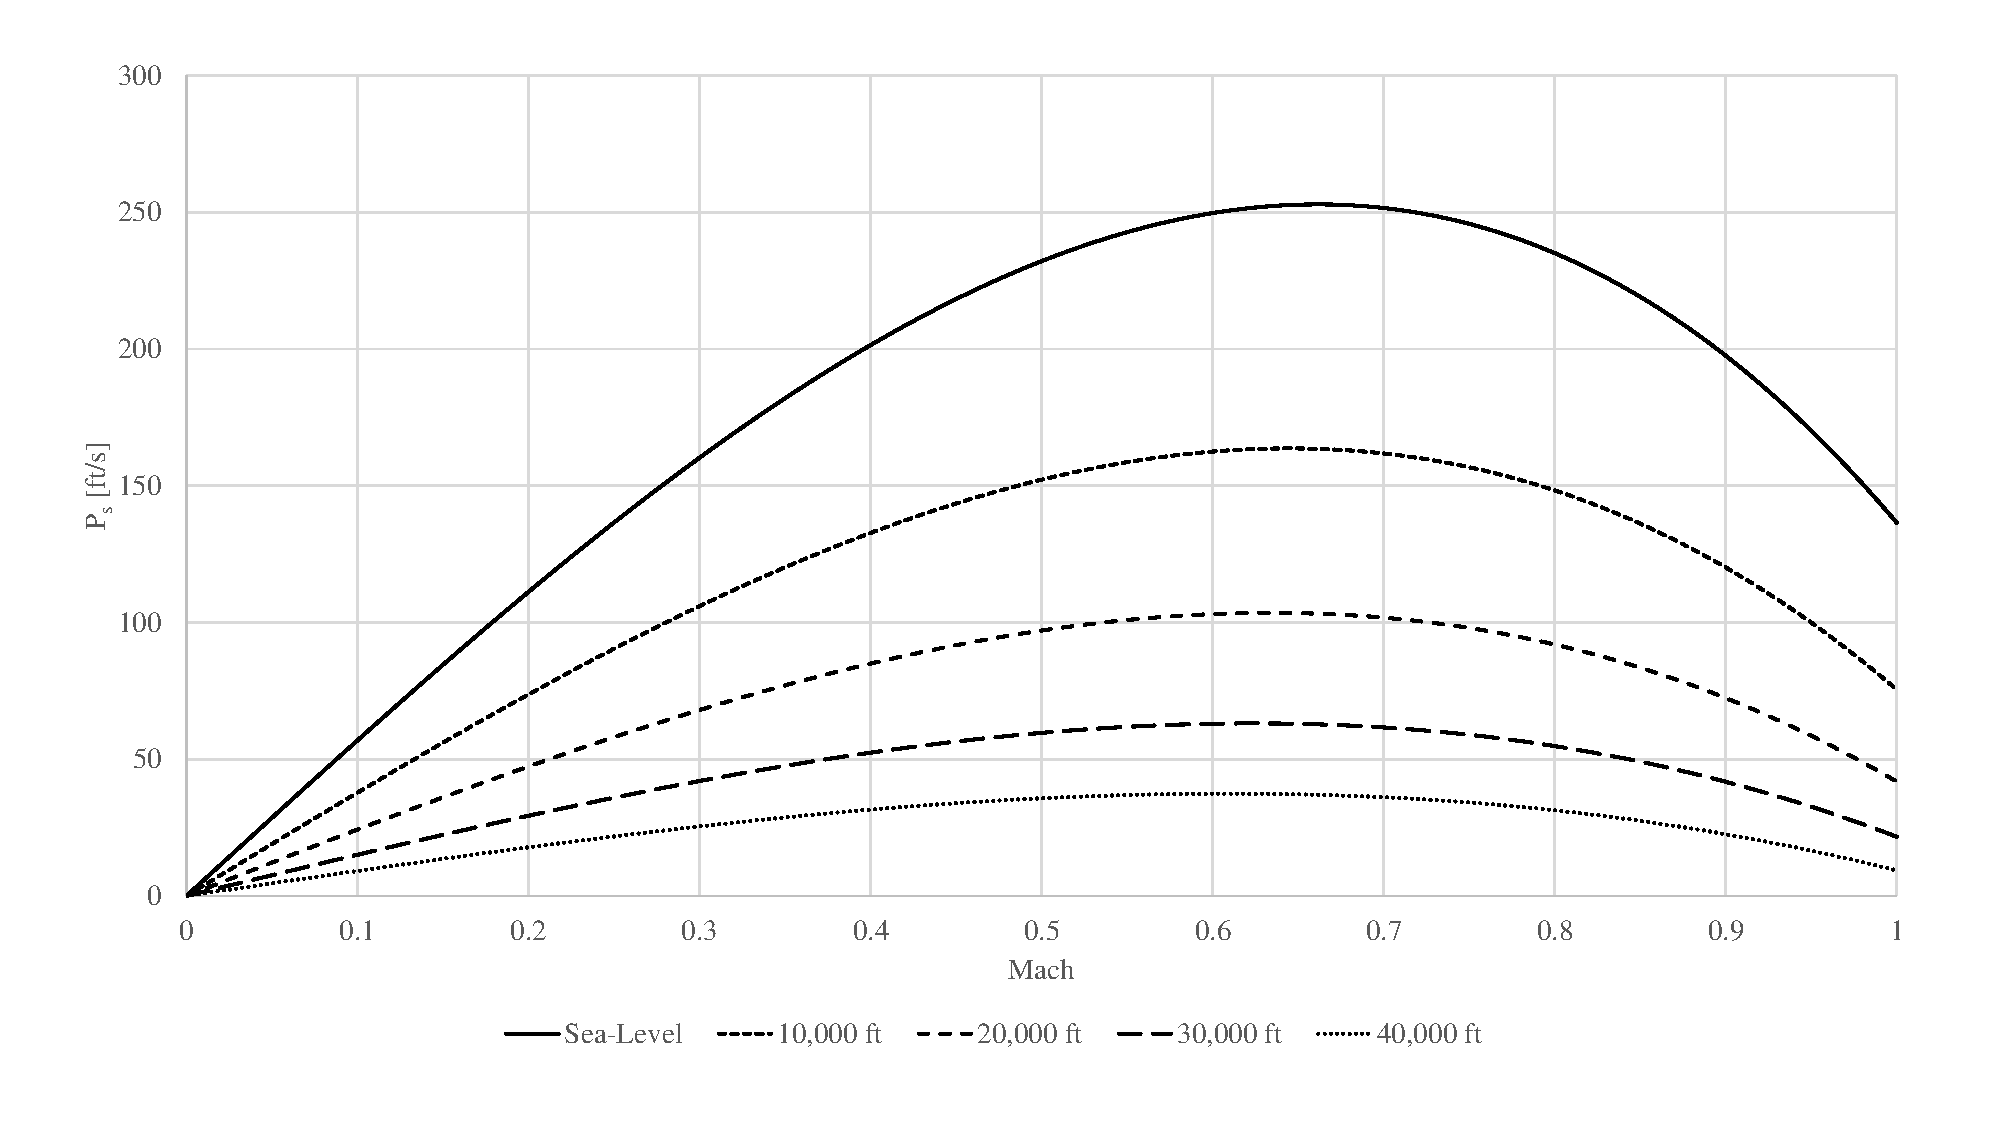
\includegraphics[width=1.0\textwidth]{Photos/Specific_Excess_Power.pdf}
    \caption{Specific Excess Power Diagram at Varying Speeds and Altitudes}
    \label{spexpw}
 \end{figure}
\clearpage

\subsection{Range-Mach Diagram}
A range-mach diagram can be used to determine the range of a particular aircraft with varying speeds while maintaining constant parameters, such as SFC, altitude, and L/D. Figure \ref{ramadg} displays this diagram at the cruising altitude of 37,000 ft. The Breguet Range equation was used to generate this plot, which follows a linear pattern. 

\begin{figure}[H]
    \centering
    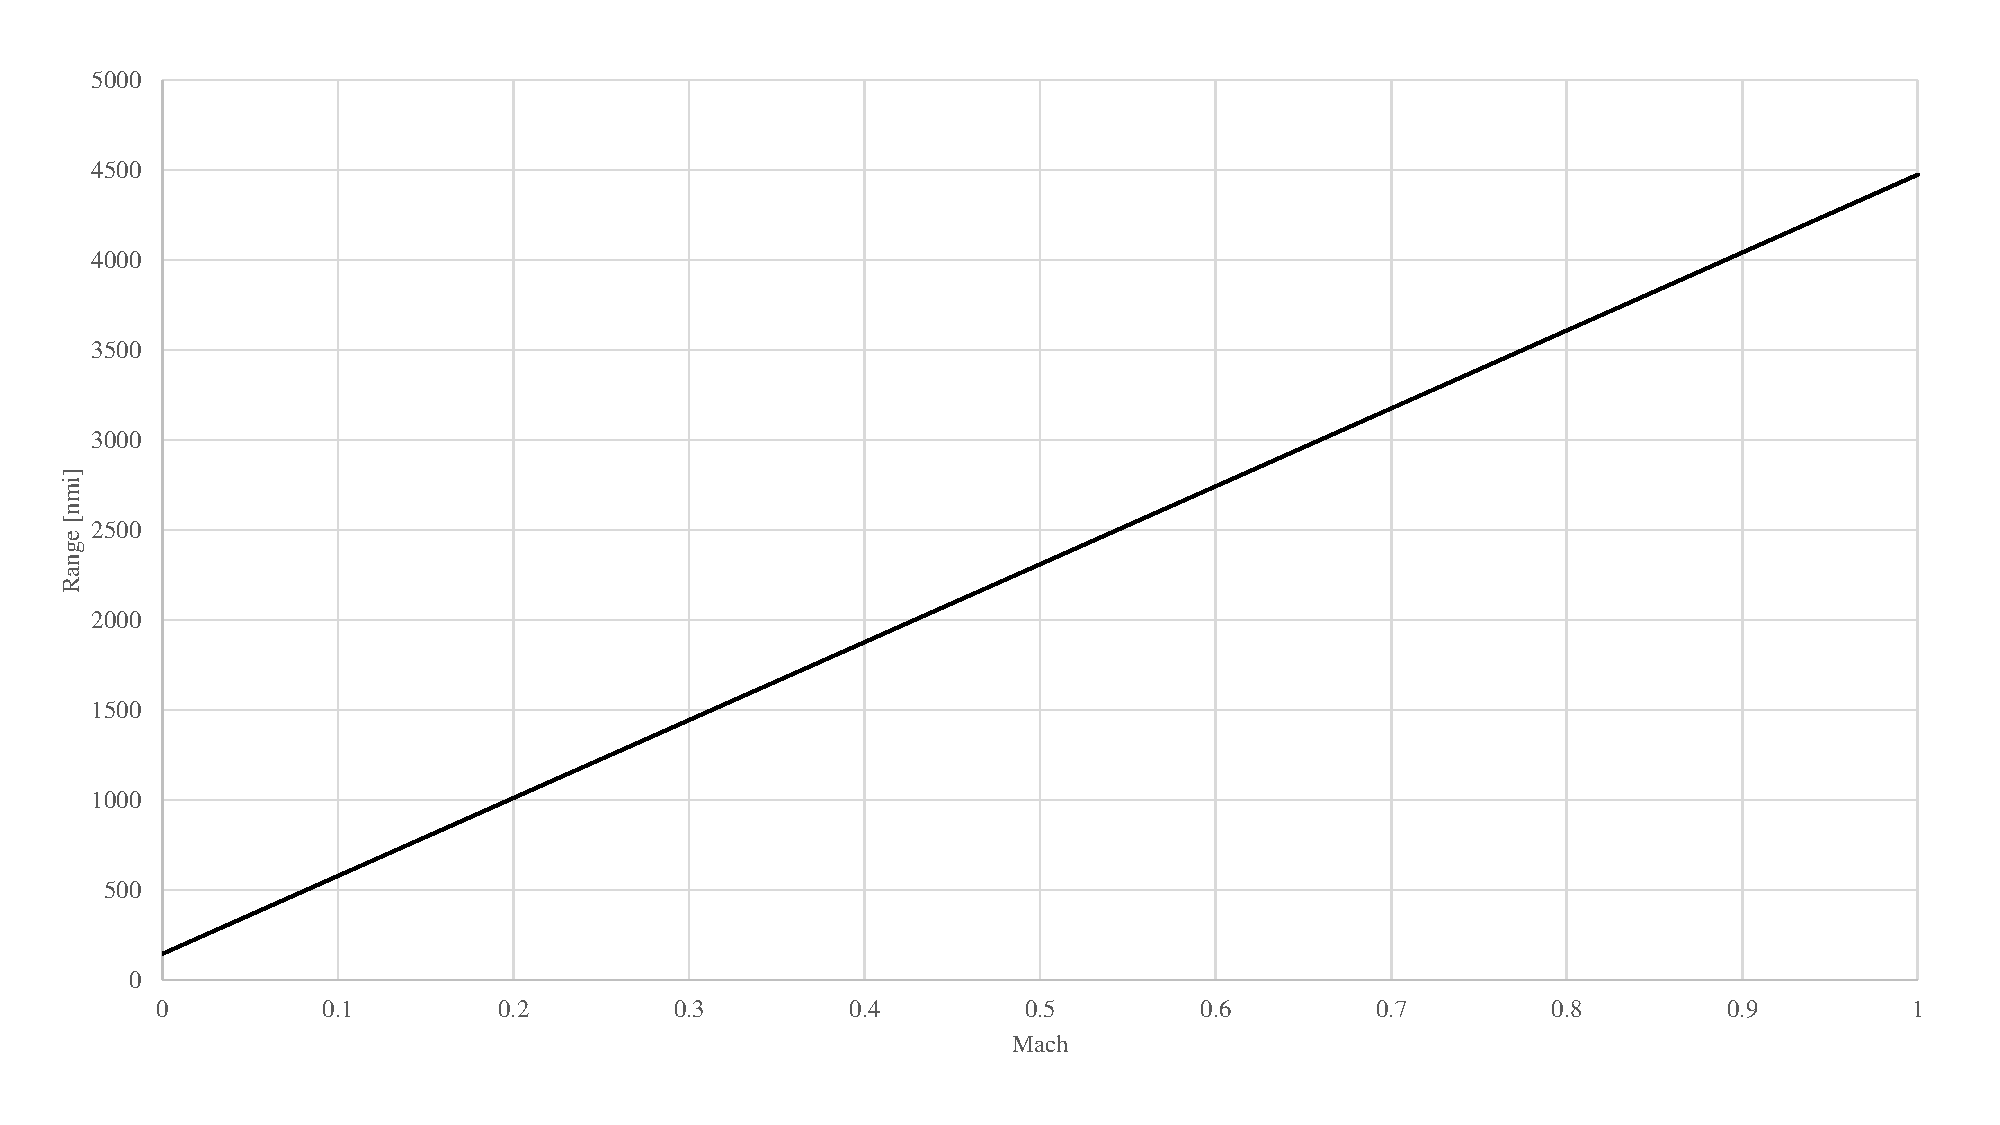
\includegraphics[width=1.0\textwidth]{Photos/Range_Mach.pdf}
    \caption{Range Mach Diagram @ 37,000 ft}
    \label{ramadg}
 \end{figure}

\subsection{Cruise and Loiter Performance Coefficients}
There are two main performance coefficients that are useful in determining the performance during loiter and cruise: $(\frac{C_{L}}{C_{D}})_{max}$ and $(\frac{C_{L}^{1/2}}{C_{D}})_{max}$. The coefficients correspond to the maximum endurance, or loiter, time and maximum range, or cruise, distance, respectively. By using the parabolic drag polar model, these coefficients become solely functions of the aircraft's geometry and $C_{D_{o}}$. Once these coefficients were obtained, the maximum endurance and range were calculated using the Breguet Endurance and Breguet Range equations, respectively. Table \ref{tab:loitcrui} displays the coefficient values as well as the maximum endurance and range. From Table \ref{tab:loitcrui}, our aircraft meets the requirements set forth by the RFP \cite{RFP}.

\begin{table}[!h]
    \centering
    \caption{Performance Coefficients with Max Endurance and Range}
    \begin{tabular}{|c|c|c|c|}\toprule 
    \boldmath{$(\frac{C_{L}}{C_{D}})_{max}$} & \boldmath{$(\frac{C_{L}^{1/2}}{C_{D}})_{max}$} & \textbf{Max Endurance [hr]} & \textbf{Max Range [NM]} \\ \hline \hline
    16.8 & 23.9 & 7.67 & 4,890 \\ 
    \bottomrule
    \end{tabular}
    \label{tab:loitcrui}
\end{table}

\clearpage
% MAT MAT MAT MAT MAT MAT MAT MAT MAT I THINK IM LIKE 97% done with THE TAKE OFF CD POSSIBLY MAYBE AT LEAST EARLY CALCULATION
% This so far without wing: 0.00098708 but I'm adding this to the wing analysis in XFLR.  O yaeh we probably can get away with assumptions and then blame the stupid aero guy for being incapable of finding these coefficients T.T
%  I WOULD NEVER BLAME YA!
% AWESOME! idk if ill have time ot include it in this report but after pdr i will for sure update the sheet


% \textcolor{red}{
% \begin{itemize}
%     \item Discuss performance analysis for takeoff and landing (accounting for ground roll and obstacle clearance), rate of climb, cruise, loiter, and service ceiling.
%     \begin{itemize}
%         \item Account for alternate conditions specified in RFP (grass, altitude, etc.) and CFR 23.67 (i.e. single engine-out takeoff)
%     \end{itemize}
% \item AIAA
% \subitem A description of the design missions defined for the proposed concepts for use in
% calculations of mission performance as per design objectives. This includes the
% selection of cruise altitude(s) and cruise speed/cruise Mach supported by pertinent
% trade analyses and discussion
% \subitem Aircraft performance summaries shall be documented and the aircraft flight envelope
% shall be shown graphically.
% \subitem Payload range chart(s)
% \subitem A V-n diagram for the aircraft with identification of necessary aircraft velocities and design load factors \hl{Or Loads disc. W/ Chris}
% \item All else per Merret --> SEE COMPASS
% \item \hl{Important aerodynamic characteristics and aerodynamic performance for key mission segments and requirements AERO or PERF}
% \end{itemize}}

\clearpage
\section{Stability and Control (\textit{JC})}
\label{section: Stab and Control}
\subsection{Stabilizer Configuration}

\begin{table}[!h]
    \centering
    \caption{Stabilizer Dimensions}
    \begin{tabular}{|c||c|c|c|} \toprule
        \textbf{Description} & {\textbf{Horizontal Stabilizer}} & 
        {\textbf{Vertical Stabilizer}} & \textbf{Units}\\ \midrule \hline
        AR & 4.5 & 1.5 & $\sim$ \\ \hline
        b (\textit{span}) & 67 & 27 & ft \\ \hline 
        $s_{\text{wing}}$ (\textit{area}) & 1,000 & 500 & ft$^2$ \\ \hline
        c/4 Sweep & 35 & 35 & degree \\ \hline
        $\lambda$ & 0.35 & 0.35 & $\sim$ \\ \hline
        Chord Root & 265.01 & 324.58 & in \\ \hline
        Chord Tip & 92.76 & 113.60 & in \\ \hline   
        Mean Aerodynamic Chord & 192.71 & 236.02 & in \\ \bottomrule
    \end{tabular}
    \label{tab:wingsizing}
\end{table}

Both the horizontal stabilizer \hl{edit out early stages etc} and vertical stabilizer are at very early stages in sizing.  Location of the stabilizers, as notated as the distance between the $\text{MAC}_{\text{wing}}$ and $\text{MAC}_{\text{stabilizers}}$, is likely to change after further stability analysis.

\subsubsection{Horizontal Stabilizer}
SAM Mk I uses a standard tail configuration.  The horizontal stabilizer is initially sized to be 25\% of $S_{wing}$.  This provides a starting point from which to begin stability analysis.  Use of an inverted NASA SC(2)-0412 airfoil for the horizontal stabilizer is proposed to provide a counter moment to the lifting effects of the wing.
\begin{figure}[!h]
    \centering
    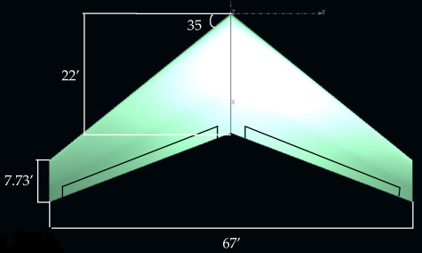
\includegraphics[width=0.75\textwidth]{Photos/stab/htail.png}
    \caption{Horizontal Stabilizer Top View}
    \label{fig:htailstab}
\end{figure}

\subsubsection{Vertical Stabilizer}
The vertical stabilizer is sized to be approximately 12.5\% of $S_{wing}$.  Additional attention must be directed at the vertical stabilizer to ensure directional stability.

\subsection{Control Surfaces}
Several control surfaces are built into the wing, horizontal stabilizer, and vertical stabilizer.  The main wing contains a flap mechanism from spanwise locations $11.5$ ft to $69.1$ ft and deflects a maximum of $\delta_F = 30\degree$.  An initial aileron sizing has determined potential placement from $72$ ft to $90$ ft.  The aileron deflection angle range has yet to be sized and will depend on performance decision for roll speed.  A trade study is currently underway to determine whether SAM Mk I should lock ailerons and implement flaperons for the transonic cruise stage.  The rudder is located on the vertical tail and spans the entire length of the tail, $27$ ft, as is normal in comparable aircraft.  The elevators are located on the horizontal stabilizer and spans from $2$ ft to $65$ ft.  Yet another trade study is taking place to determine the selection of trim tabs or a trimmable horizontal stabilizer.

\clearpage
% \subsection{Pitch Trim Control}

% \subsection{Longitudinal Static Stability}

% \subsection{Stability Control Derivatives}


% \subsubsection{$C_{L,\alpha}$}

% \subsubsection{$C_{m,\alpha}$}

% \subsubsection{$C_{m,\delta e}$}

% \subsubsection{$\varepsilon_\alpha$}

% \textcolor{red}{
% \begin{itemize}
%     \item Discuss rationale for stabilizer configuration (if not done in Configuration section).
%     \item Provide reasoning and methodologies for sizing of all stabilizers, with relevant sources.
%     \begin{itemize}
%         \item Notch/scissor diagram (not required for PDR but will be for FDR)
%         \item Discuss airfoil selection with reasoning (e.g. symmetry).
%         \item Include explicit values for both horizontal and vertical stabilizers: span, root chord, tip chord, (quarter chord) sweep, area, (leading edge) location, volume coefficient
%         \item Provide scaled visual representations of all stabilizers (top-down view for horizontal, side view for vertical).
%         \begin{itemize}
%             \item The following parameters should be shown within the diagrams: span, root chord, tip chord, and sweep.
%         \end{itemize}
%     \end{itemize}
%     \item Provide reasoning and methodologies for sizing of all control surface, with relevant sources.
%     \begin{itemize}
%         \item Include explicit values for all control surfaces (e.g. elevator, ailerons, rudder, and flaps): chord ratios and lengths, span ratios and lengths, and deflection range (min/max).
%         \item Provide scaled visual representations of all control surfaces (can use SAM e diagrams as those for stabilizers).
%         \begin{itemize}
%             \item The following parameters should be shown within the diagrams: span, root chord, and tip chord.
%         \end{itemize}
%     \end{itemize}
%     \item Include incidence values for both the wing and horizontal stabilizer, with reasoning.
%     \item Provide trim diagrams with established trim points and elevator/stabilizer deflections.
%     \begin{itemize}
%         \item Have separate diagrams for takeoff, cruise, and landing.
%         \item Plot lines for at least 3 different elevator deflections (with indications in key).
%         \item Mark each trim point on its respective diagram.
%         \item Indicate takeoff, cruise, and landing deflections as interpolated, with $C_L$ values.
%     \end{itemize}
%     \item Discuss longitudinal static stability.
%     \begin{itemize}
%         \item Indicate static margin range and fore and aft CG locations used to find range.
%         \item Indicate neutral point location with calculation method.
%     \end{itemize}
%     \item Provide a list of stability control derivatives used in all calculations, with methodologies.
%     \begin{itemize}
%         \item Include (at minimum): $C_{L,\alpha}, C_{m,\alpha}, C_{m,\delta e},\varepsilon_{\alpha}$
%     \end{itemize}
%     \item Include at least two trade studies that use quantitative analysis to support design decisions made.
%     \item Discuss parachute incorporation if required.
%     \item Discuss future work.
%     \item \hl{AIAA: Summary of basic stability and control characteristics; this should include, but is not limited to static margin, pitch, roll and yaw derivatives}
% \end{itemize}}

\clearpage
\section{Structures and Loads}
\label{section: Structures and Loads}
\subsection{Structures (\textit{CE})}
\subsubsection{Material Selection (\textit{CE})}
Modern-age aircraft exhibit many different structure layouts and material selection for each structure of the aircraft. The goal for the material selection for each section of the aircraft is to meet the given requirements, as well as provide an aircraft which will have the best mechanical performance for the given flight missions. The different structure types evaluated are tabulated in Table \ref{tab:structure_material_table}.

\begin{table}[!h]
\centering
\caption{Structures Build-up Descriptions }
\label{tab:structure_material_table}
\begin{tabular}{ |p{2cm}||p{13cm}| }
\toprule
\multicolumn{1}{|c||}{\textbf{Build-up Type}} & \multicolumn{1}{c|}{\textbf{Description}}                                                                                                                       \\ \hline\hline
Metal                                       & Most or all parts of the primary and secondary structure are metallic, such as aluminum, steel, and titanium alloys                                             \\ \hline
Composite                                    & Most or all parts of the primary and secondary structure are composite, such as carbon fiber reinforced polymers (CFRP), fiberglass, or other composites \\ \hline
Hybrid                                       & Depending on the structure, the material of the structure is either metal or composite                                                                            \\ \bottomrule
\end{tabular}
\end{table}
% \begin{tabular}{ |p{3cm}||p{3cm}|p{3cm}|p{1.5cm}|p{3cm}| }

A metallic build-up is the more traditional method of designing aircraft structures, where most or all primary structures are composed of metal alloys like aluminum, steel, and titanium. This method of construction is typically cost-effective and weight efficient for most structures, however, there are downsides such as damage tolerance and fatigue. A composite build-up requires relatively high development and manufacturing costs using modern technology, but can offer incredible weight-savings and operational cost savings compared to metal structure due to their high strength-to-weight ratio and fatigue and damage tolerance resistance. 

A hybrid build-up is a method where both metals and composites are used for different structures depending on key factors such as fatigue, damage tolerance, ultimate strength per density ratio, cost of manufacturing, assembly methods, and operational costs. Hybrid designs usually reduce overall costs and empty weight of the structure, which results in the wings and stabilizers to be a mainly composite build-up and the fuselage and other secondary structures to be a metal build-up. Hybrid construction is a newer technology, and as the development of manufacturing of composites advances, this style of construction may become more prevalent in industry. A notable aircraft which uses a hybrid build would be the Boeing 777X, in which the wings and stabilizers are composite and the fuselage is metallic. The reason the fuselage is metallic and not composite comes down to the difficulties in manufacturing a round and continuous composite structure, such as the fuselage and empennage sections. A notable aircraft which utilizes mainly composite construction, however, is the Boeing 787. The B787 encountered enormous program overruns in costs and time, mainly stemming from the fuselage construction.

In Table \ref{tab:pugh_structures}, the benefits and costs for each build-up construction method were weighed in a Pugh matrix given the requirements such as cost, manufacturing, and mechanical properties. Cost was weighted the highest due to the RFP requirement which states the proposed aircraft must reduce costs \cite{RFP}.

\begin{table}[!h]
\centering
\caption{Pugh Matrix for Structures Material Selection}
\begin{tabular}{|p{3.5cm}||p{2cm}|p{2cm}|p{2cm}|p{2cm}| }
\toprule
\multicolumn{1}{|c||}{\textbf{Criteria}} & \multicolumn{1}{c|}{\textbf{Weight}} &  
\multicolumn{1}{c|}{\textbf{Metallic}} & \multicolumn{1}{c|}{\textbf{Composite}} & \multicolumn{1}{c|}{\textbf{Hybrid}} \\ \hline \hline 
Cost & 10 & 9 & 7 & 8 \\ \hline
Manufacturability & 8 & 8 & 5 & 7 \\  \hline
Strength to Weight & 8 & 7 & 8 & 9 \\  \hline
Fatigue Rating & 5 & 6 & 8 & 7 \\  \hline
Damage Tolerance & 5 & 7 & 6 & 7 \\  \hline
Corrosion Resistance & 4 & 4 & 9 & 8 \\  \hline
Environmental Impact & 3 & 8 & 4 & 6 \\  \hline \hline
 & \textbf{Total} & \textbf{315} & \textbf{292} & \textbf{328} \\
\bottomrule
\end{tabular}
\label{tab:pugh_structures}
\end{table}
\FloatBarrier

Given the qualitative Pugh matrix, a hybrid construction is most ideal for the given aircraft requirements. This would entail the wingbox and fuselage, including the longerons, frames, and floor joists being constructed from an aluminum alloy. The landing gear will be constructed primary from steel and titanium alloys. The wings and stabilizers, including the skins, ribs, ribs, and stringers would then be modelled using a uni-directional composite material, which assumes isotropic material properties. In reality, composites are anisotropic, but analysis of a directional layup composite is very difficult and not in the scope of this preliminary design. 

In Table \ref{tab:material_selection}, the material composition of each structure can be seen. It can be noticed that all primary structure uses carbon fiber reinforced polymer (CFRP) and epoxy, fiberglass and epoxy, aluminum, steel, or titanium alloys.

% Method 1
\begin{table}[!h]
\centering
\caption{Primary Structure Material Composition}
\begin{tabular}{|p{3.5cm}||p{2cm}|p{6cm}| }
\toprule
\multicolumn{1}{|c||}{\textbf{Structure}} & \multicolumn{1}{c|}{\textbf{Components}} & \multicolumn{1}{c|}{\textbf{Material}} \\ \hline \hline 
\multirow{4}{*}{Wing} & Skin & \multirow{4}{*}{CFRP/Epoxy} \\
                     & Ribs & \\
                     & Spars & \\
                     & Stringers & \\ \hline
\multirow{4}{*}{Horizontal Stabilizer} & Skin & \multirow{4}{*}{CFRP/Epoxy or Fiberglass/Epoxy} \\
                     & Ribs & \\
                     & Spars & \\
                     & Stringers & \\ \hline
\multirow{4}{*}{Vertical Stabilizer} & Skin & \multirow{4}{*}{CFRP/Epoxy or Fiberglass/Epoxy} \\
                     & Ribs & \\
                     & Spars & \\
                     & Stringers & \\ \hline
\multirow{4}{*}{Fuselage} & Skin & \multirow{4}{*}{2024-T4 Aluminum} \\
                     & Longerons & \\
                     & Frames & \\
                     & Wingbox & \\ \hline
\multirow{3}{*}{Landing Gear} & Struts & \multirow{3}{*}{Aluminum, Steel, or Titanium Alloys} \\
                     & Axles & \\
                     & Bulkheads & \\ \hline
\bottomrule
\end{tabular}
\label{tab:material_selection}
\end{table}

% Method 2
\begin{table}[!h]
\centering
\caption{Primary Structure Material Composition}
\begin{tabular}{|p{3.5cm}||p{2cm}|p{6cm}|}\toprule
\textbf{Structure} & \textbf{Components} & \textbf{Material} \\ \hline \hline 

    Wing & Skins \newline Ribs \newline Spars \newline Stringers & CFRP/Epoxy \\ \hline
    Horizontal Stabilizer & Skins \newline Ribs \newline Spars \newline Stringers & CFRP/Epoxy or Fiberglass/Epoxy \\\hline
    Vertical Stabilizer & Skins \newline Ribs \newline Spars \newline Stringers & CFRP/Epoxy or Fiberglass/Epoxy \\\hline
    Fuselage & Skins \newline Longerons \newline Frames \newline Wingbox & 2024-T4 Aluminium \\\hline
    Landing Gear & Struts \newline Axles \newline Bulkheads & Aluminium, Steel, or Titanium Alloys \\ \bottomrule

\end{tabular}
\label{tab:material_selection}
\end{table}

For analysis, the CFRP material chosen was 

\subsubsection{Construction and Layout (\textit{CE})}
Given the hybrid construction method, the wings and stabilizers require a newer method of construction compared to the traditional metallic construction. Since composite layups are essentially an additive manufacturing technique, the stringers can be integrated into the upper and lower panels of the wings and stabilizers. This alone saves incredible costs and weight by eliminating the use of fasteners in high-load locations. The absence of fasteners increases the damage tolerance and fatigue rating of the structure as well.

Spars are the most important structure to the wings, and arguably the most important on the entire aircraft. These few parts make the entire aircraft fly, and in the process, see a lot of loading cycles over the life of the aircraft. In metal structures, loading cycles cause fatiguing, and then fatigue cracking, which degrades the structure. Traditionally, metallic structures use a 3-piece build-up for the spar: chord on the top and bottom, and a web connecting the two chords. This structure ends-up looking like a C-channel extrusion. The reason the spars are a 3-piece build-up comes down to crack growth and fatigue. A crack starts in the lower chord, but cannot grow through the entire spar since the chord is connected to the web by fasteners. There are a few aircraft that have used a one-piece, or monolithic, metallic spar, some being the Boeing 1-B and the Airbus 320 NEO. There is significant research in learning crack-growth patterns and predicting where cracks will start and grow; opening-up huge possibilities in reducing manufacturing costs by allowing optimized metallic spars to be utilized on low-cost aircraft.

\newpage
The spars are where composites differ greatly from traditional 3-piece spar construction. Since composite structures do not crack like metal structures when fatigued, a monolithic spar can be utilized. This spar construction reduces costs, but increases the weight due to a thicker layup compared to a simpler 3-piece construction. Due to the considerable cost savings, a monolithic composite spar was modelled, seen in Fig. \ref{fig:spar_layout}.

\begin{figure}[!h]
    \centering
    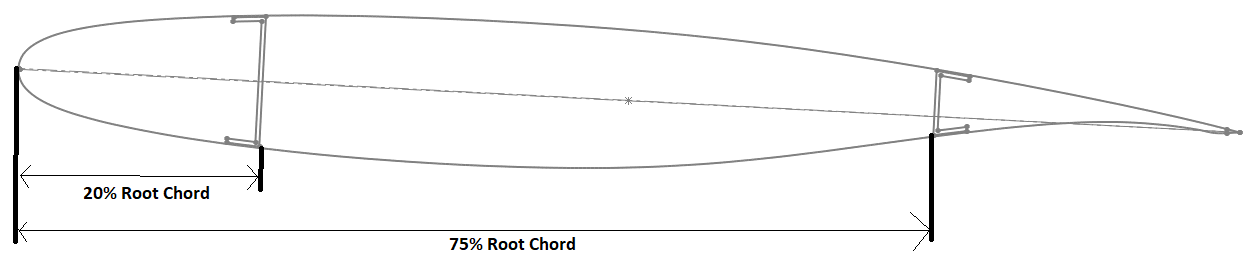
\includegraphics[width=\linewidth]{Photos/structuresandloads/Spar Layout.PNG}
    \caption{SAM Mk. I Spar Cross Section at the Root Chord}
    \label{fig:spar_layout}
\end{figure}

Ribs in the wings are traditionally multi-piece substructures comprised of machined aluminum parts. The benefit to using aluminum ribs in the wing comes from the fact that composites are difficult to utilize on very complex and dramatic geometry. However, due to manufacturing costs, a multi-piece composite rib was chosen over a monolithic metallic rib. In an effort to save more cost and manufacturing troubles, a monolithic rib structure, with the rib posts, chords, webs, and pads formed in a single composite part, can be investigated at a later date. Ribs in the stabilizers are typically not as complex as a rib in the wings due to the lower-loaded and smaller structure. In the stabilizers, composite ribs may be utilized for weight savings. The current rib spacing is 30 inches, which is a derivative of the approximation given by Raymer with a slight adjustment for composite composition. A more detailed analysis is needed to improve spacing and sizing of the ribs \cite{raymer}. \hl{would hide the more detailed is needed stuff; tildes don't show up unless you type (see below)}
$\sim$

Since the fuselage is a metallic structure, a common layout of frames, stringers, and floor joists can be utilized. The floor joists may be a composite part, as the joists are not primary structure, and the connection method to the frames of the fuselage is by brackets and fasteners. Frames in the business class are spaced with the same distance of the business class seat pitch, and the economy frames are spaced the same distance of the economy seat pitch. The seat pitches are defined in Section \ref{section: internal config}. The frames and stringers are spaced such that no windows or exit doors are covered or physically blocked. Several frames will be considered "floating", or not connected to the skin of the fuselage, and others being traditional frames. The floating frames are only mounted to the stringers, rather than the actual skin of the fuselage. Floating frames increase fatigue life, as fewer holes are introduced into the fuselage skin. It will also need to be noted that frames cannot be present where emergency exit doors and windows exist.

In Fig. \ref{fig:structure_cutaway}, the aircraft structure can be seen. It should be noticed that no windows or doors are covered by frames or stringers in the fuselage. Also note that at this time, the nose ribs have not been modelled, as their current spacing and size is not fully defined at this time.

\begin{figure}[!h]
    \centering
    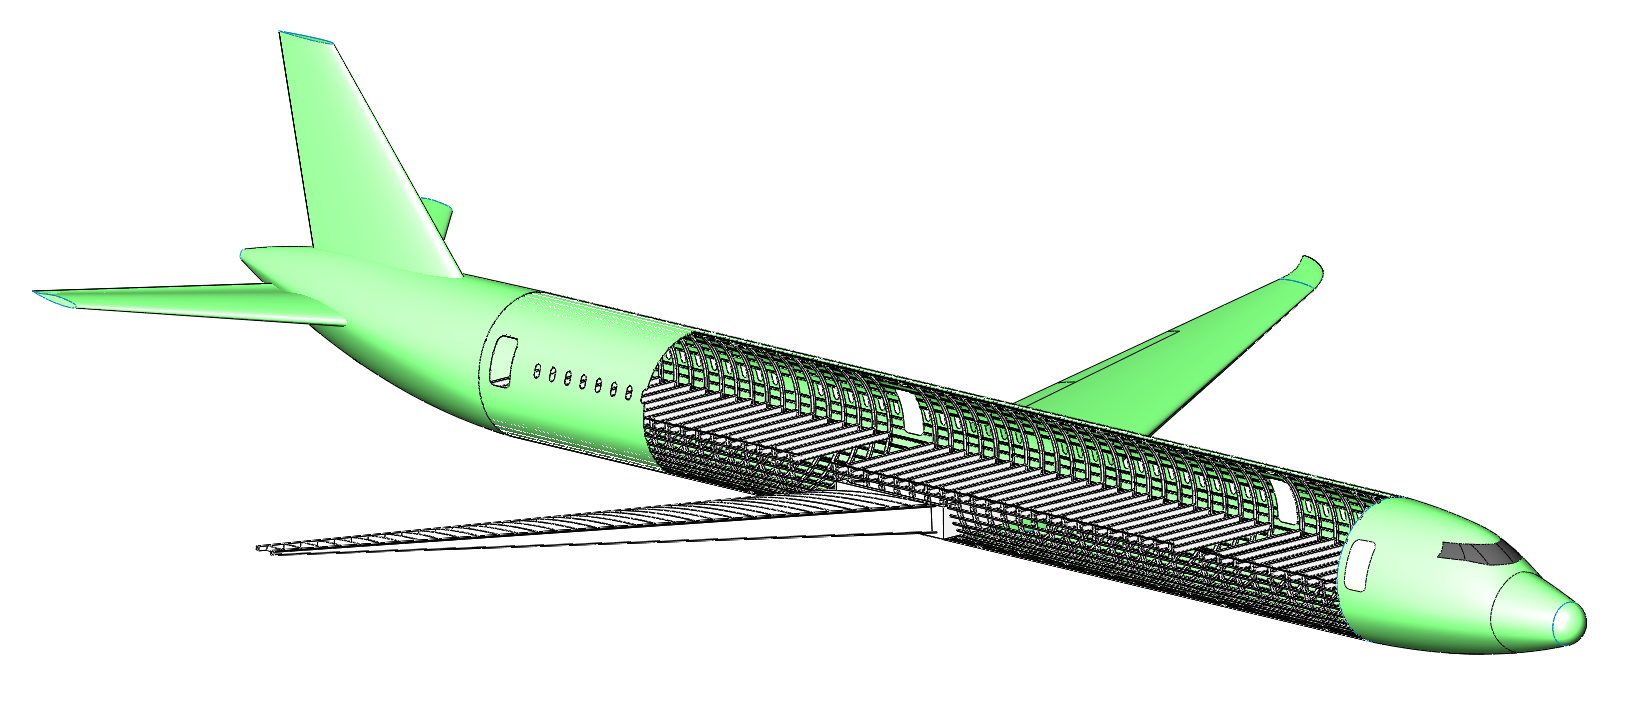
\includegraphics[width=\linewidth]{Photos/structuresandloads/Updated Sctructures Cutaway.PNG}
    \caption{SAM Mk. I Structures Model Cutaway}
    \label{fig:structure_cutaway}
\end{figure}

\subsubsection{Wing Attachment and Configuration}
There are two primary methods of mating the wings and the fuselage: "bolt-on" and "drop-in". These methods are both commonly used in industry, as both offer different advantages and carry their own disadvantages. 

A "bolt-on" method essentially bolts the wings onto the fuselage through the wingbox, as the wingbox is integrated into the fuselage. Utilizing shear plates or tension bolts, each wing is attached to the fuselage using fasteners. This method is preferred by most aircraft manufactures, as manufacturing of the fuselage with an integral wingbox and two separate wings is easier to manage in an assembly line in most cases. Using fasteners to attach the wing to the fuselage from the outside poses a difficult engineering challenge which is to make sure load paths are correctly transferring load to the correct primary structures.

The "drop-in" method refers to dropping the fuselage into the space made by the wingbox and wing superstructure. In this method, the wings and wingbox are a singular structure, and the fuselage does not have an integral wingbox. Due to the wings and wingbox being connected before the mating to the fuselage, a more robust connection to the wingbox (internal connection of the spars to the wingbox, rather than fasteners) can be achieved. 

Given that the aircraft is a wide-body, large wingspan structure, a bolt-on method would be preferred, as the manufacturing and logistical challenges in a "drop-in" method are costly. Choosing to use the bolt-on method, the wing was then designed accordingly. In Fig. \ref{fig:wing_structure}, the wing and wingbox structure can be seen.

\begin{figure}[!h]
    \centering
    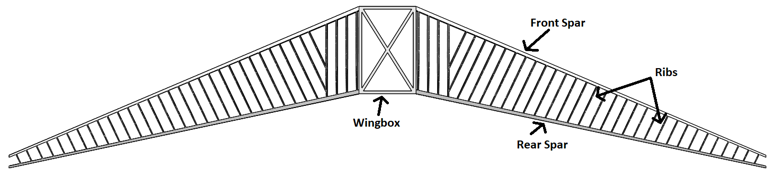
\includegraphics[width=\linewidth]{Photos/structuresandloads/Wing Structure.PNG}
    \caption{SAM Mk. I Wing Structure Top View}
    \label{fig:wing_structure}
\end{figure}
\FloatBarrier

It can also be seen in Fig. \ref{fig:wing_structure} that the ribs of the wing are currently modelled such that they are parallel to the stream-wise direction. Typically this is unconventional, as stress risers form at the rib and spar junction (at the rib posts). A more structurally sound and easy to manufacture configuration would be to align the ribs to be perpendicular to the quarter-chord or front spar.

\subsubsection{Future Work for Structures (\textit{CE})}
Future work includes several key tasks. First item to tackle is carrying-out a full FEA analysis on the wing and fuselage. In the CAD model, the structure of the aircraft needs to be improved by adding more detail to the stabilizers and the nose cone once geometric sizing is completed, as well as change the direction of the ribs to be perpendicular to the quarter-chord or front spar to minimize costs and stress risers. Some more future work includes the creation of useful trade studies, particularly trade studies comparing the sizing of the spars and spacing of the ribs in the wing to the stiffness and weight of the wing. \hl{kill or rename}

\subsection{Loads (\textit{MK})}
\subsubsection{V-N Diagram}
\label{subvn}
One important aspect in the structural analysis of the aircraft is determining the limits in the performance of the aircraft. This is done using a V-N diagram, as shown in Figure \ref{figVN}. This diagram incorporates parameters such as wing loading and performance velocities (maneuvering, cruise, and dive velocities) along with limit loading factors. Maximum positive and negative limit loading factors of 2.50 and -1.0 were chosen, respectively, according to the regulations set forth in FAA 14 CFR Part 25.337 \cite{cfr}, Limit Maneuvering Load Factors. Additionally, gust loads were added according to CFR Part 25.341 \cite{cfr}. The gust load lines were further calculated using a safety factor of 1.5, as specified in FAA 14 CFR Part 25.303, Factor of Safety \cite{cfr}. Note that the velocities displayed in the diagram (Figure \ref{figVN}) units displayed as equivalent velocities (KEAS). This V-N diagram was created assuming sea-level conditions. 

\begin{figure}[H]
    \centering
    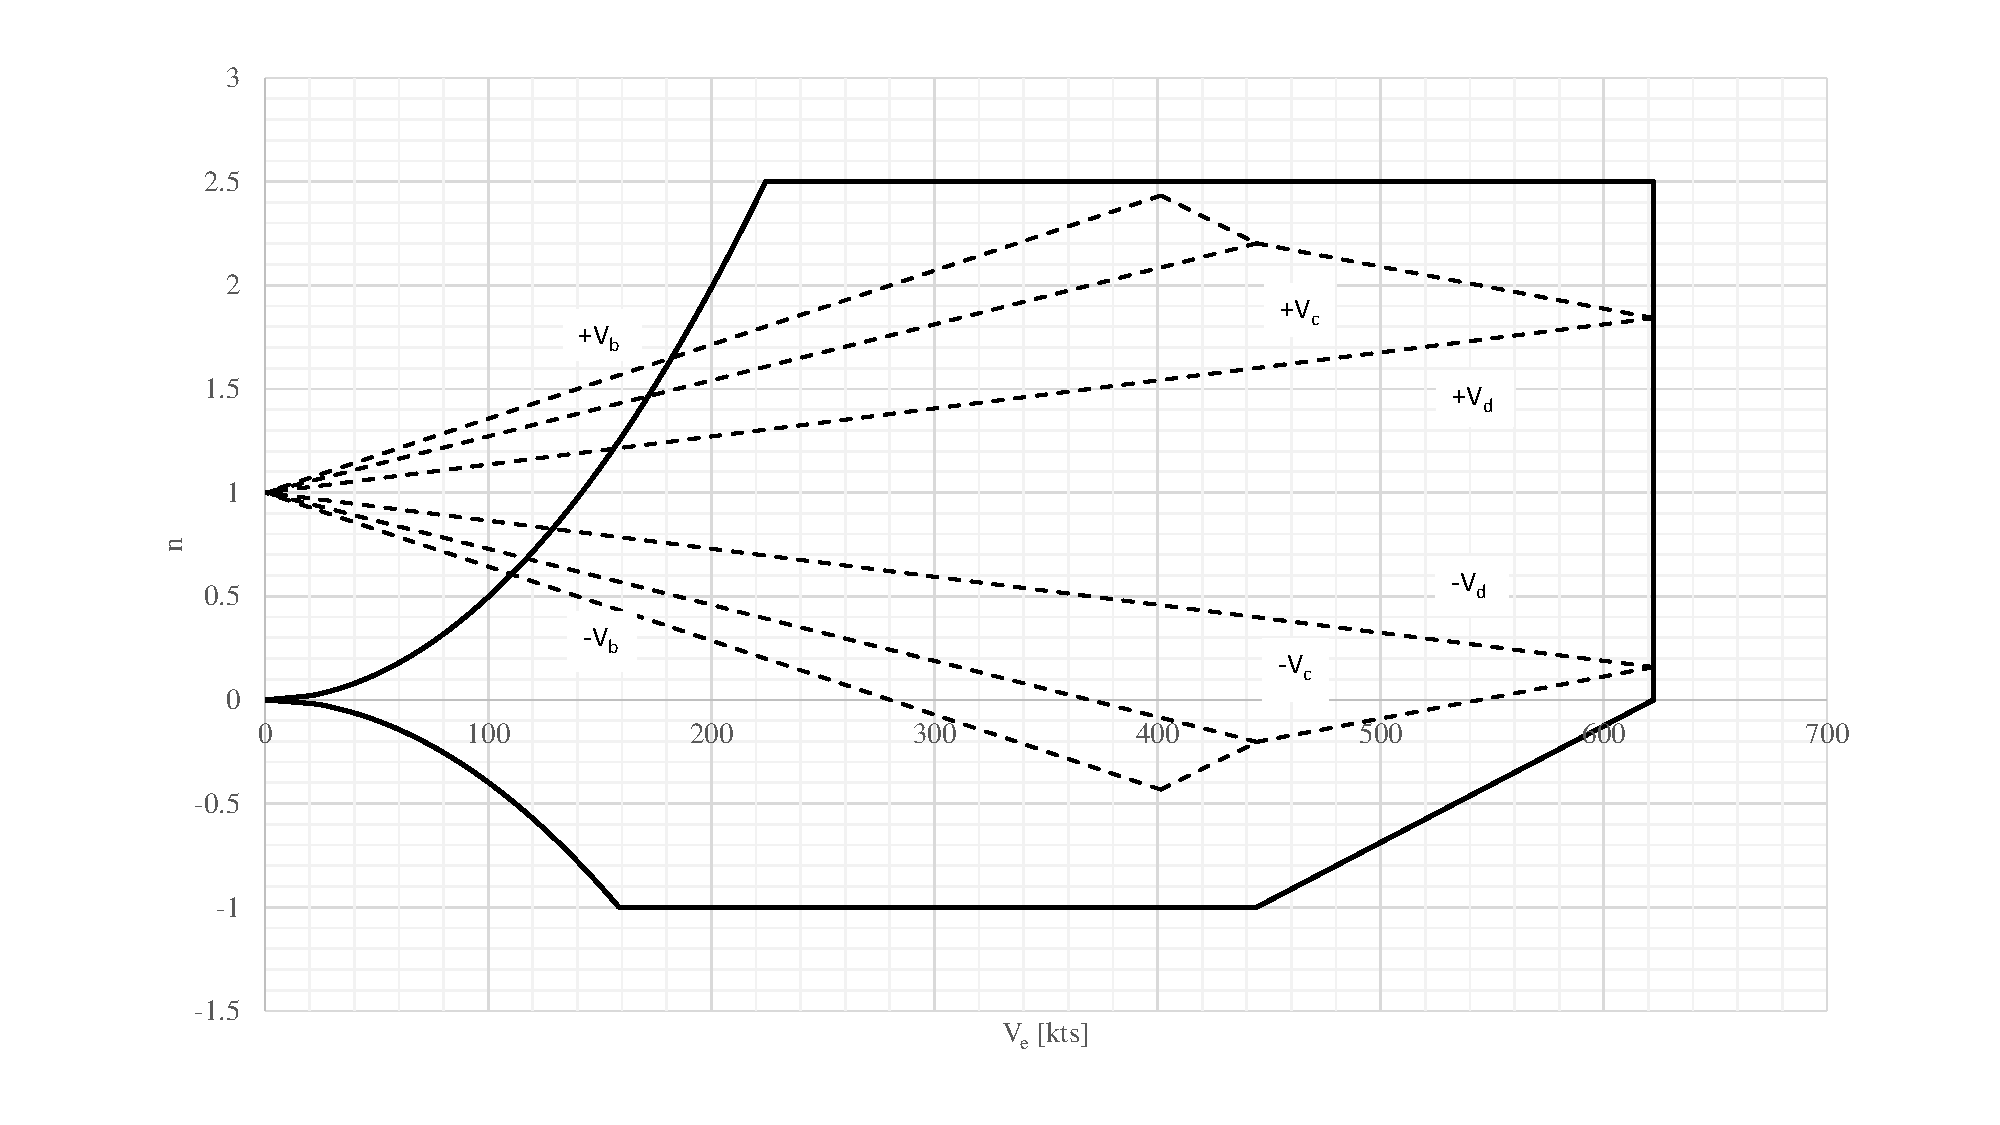
\includegraphics[width=\linewidth]{Photos/VN_Diagram.pdf}
    \caption{V-N Diagram of Limit Load Factors}
    \label{figVN}
\end{figure}

As seen from Figure \ref{figVN}, gust loads do not limit the performance of the SAM Mk. 1. Moreover, using equations from Roskam \cite{roskam_5}, design maneuvering speed ($V_{A}$), cruising speed ($V_{C}$) and design diving speed ($V_{D}$) were estimated to be 220 kts, 440 kts. and 620 kts, respectively. Furthermore, the calculation of the positive and negative stall lines involved the use of equations from Roskam \cite{roskam_5}. At sea-level and at a limit loading factor of 1 and -1, the stall speeds were calculated to be 140 kts and 160 kts, respectively.

\subsubsection{Wing Loading}
\label{winlod}
The loading experienced on the wing was analyzed. Specifically, Schrenk's approximation was used to estimate the span-wise loading on the wing, using equations found in Chapter 14 of Raymer \cite{raymer} as well as the positive limit loading factor from the V-n Diagram. First, the elliptical loading was estimated across the wing. Then, a rectangular method was used to estimate the loading on the wing. Both of these methods required the Schrenk's Approximation Set, which was estimated to be about 728,000 lb. Then, Schrenk's approximation takes the average of the elliptical distribution and a rectangular distribution to provide a semi-empirical approach to visualizing the load distribution on the wing. Figure \ref{schrenk} shows the wing loading using Schrenk's approximation along with the elliptical and rectangular approximation across half the wing, with the other half being symmetric. 

\begin{figure}[H]
    \centering
    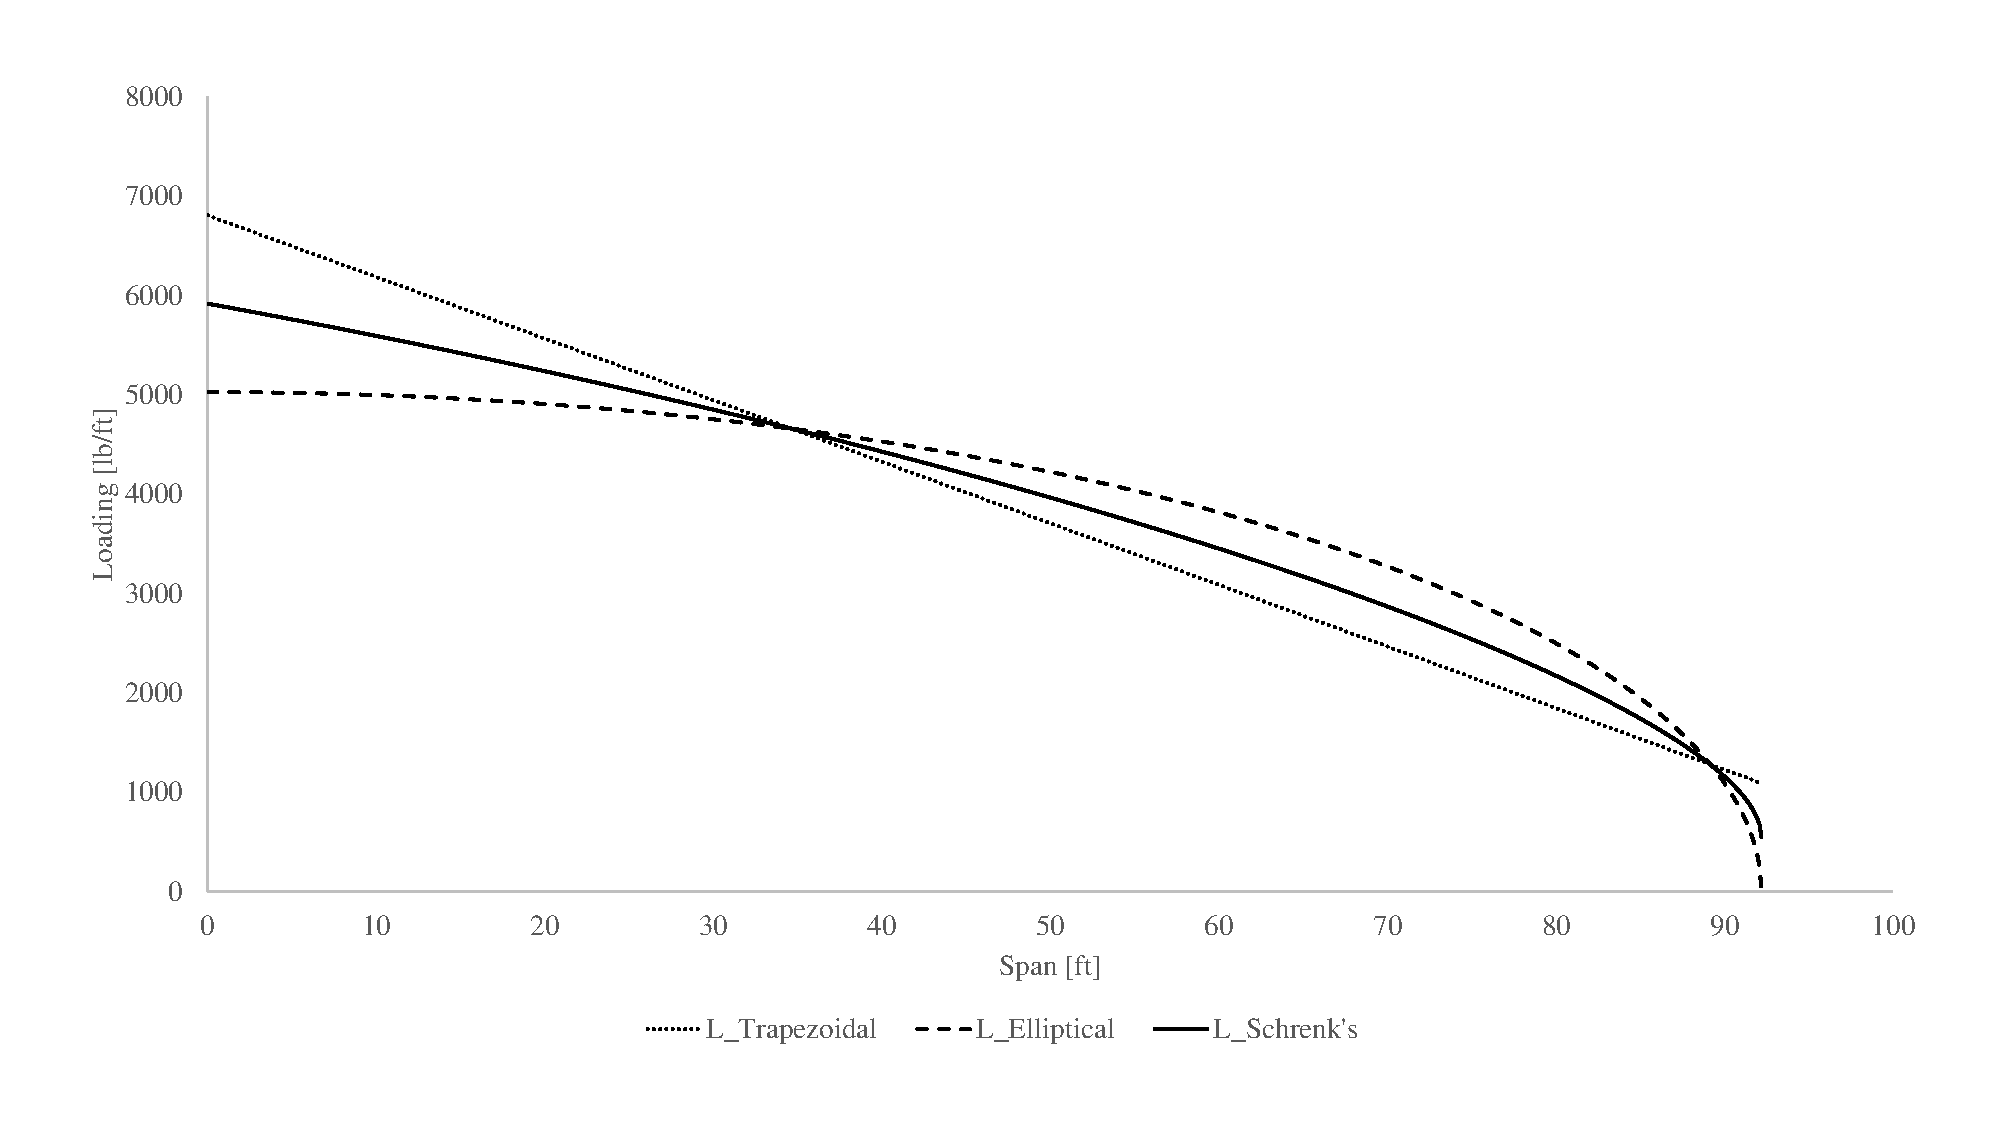
\includegraphics[width=1.0\linewidth]{Photos/Schrenks.pdf}
    \caption{Load Distribution Across the Half-span Wing}
    \label{schrenk}
\end{figure}

After estimating the load distribution on the wing, the internal forces of the wing are to be determined. Team Toucans implemented a numerical integration scheme, in which the Schrenk's diagram was integrated to obtain a shear diagram. This shear diagram was then integrated again to derive the bending moment diagram. The integration method of choice was the trapezoidal method. Both of these diagrams are modeled on the half-span of the wing, thereby assuming symmetry. Figures \ref{sheardiag} and \ref{momentdiag} show the Shear and Bending Moment diagrams as functions of half the span of the wing, respectively. Note that the shear loading and bending moments are zero at the tips and maximum at the center of the wing. 

\begin{figure}[H]
    \centering
    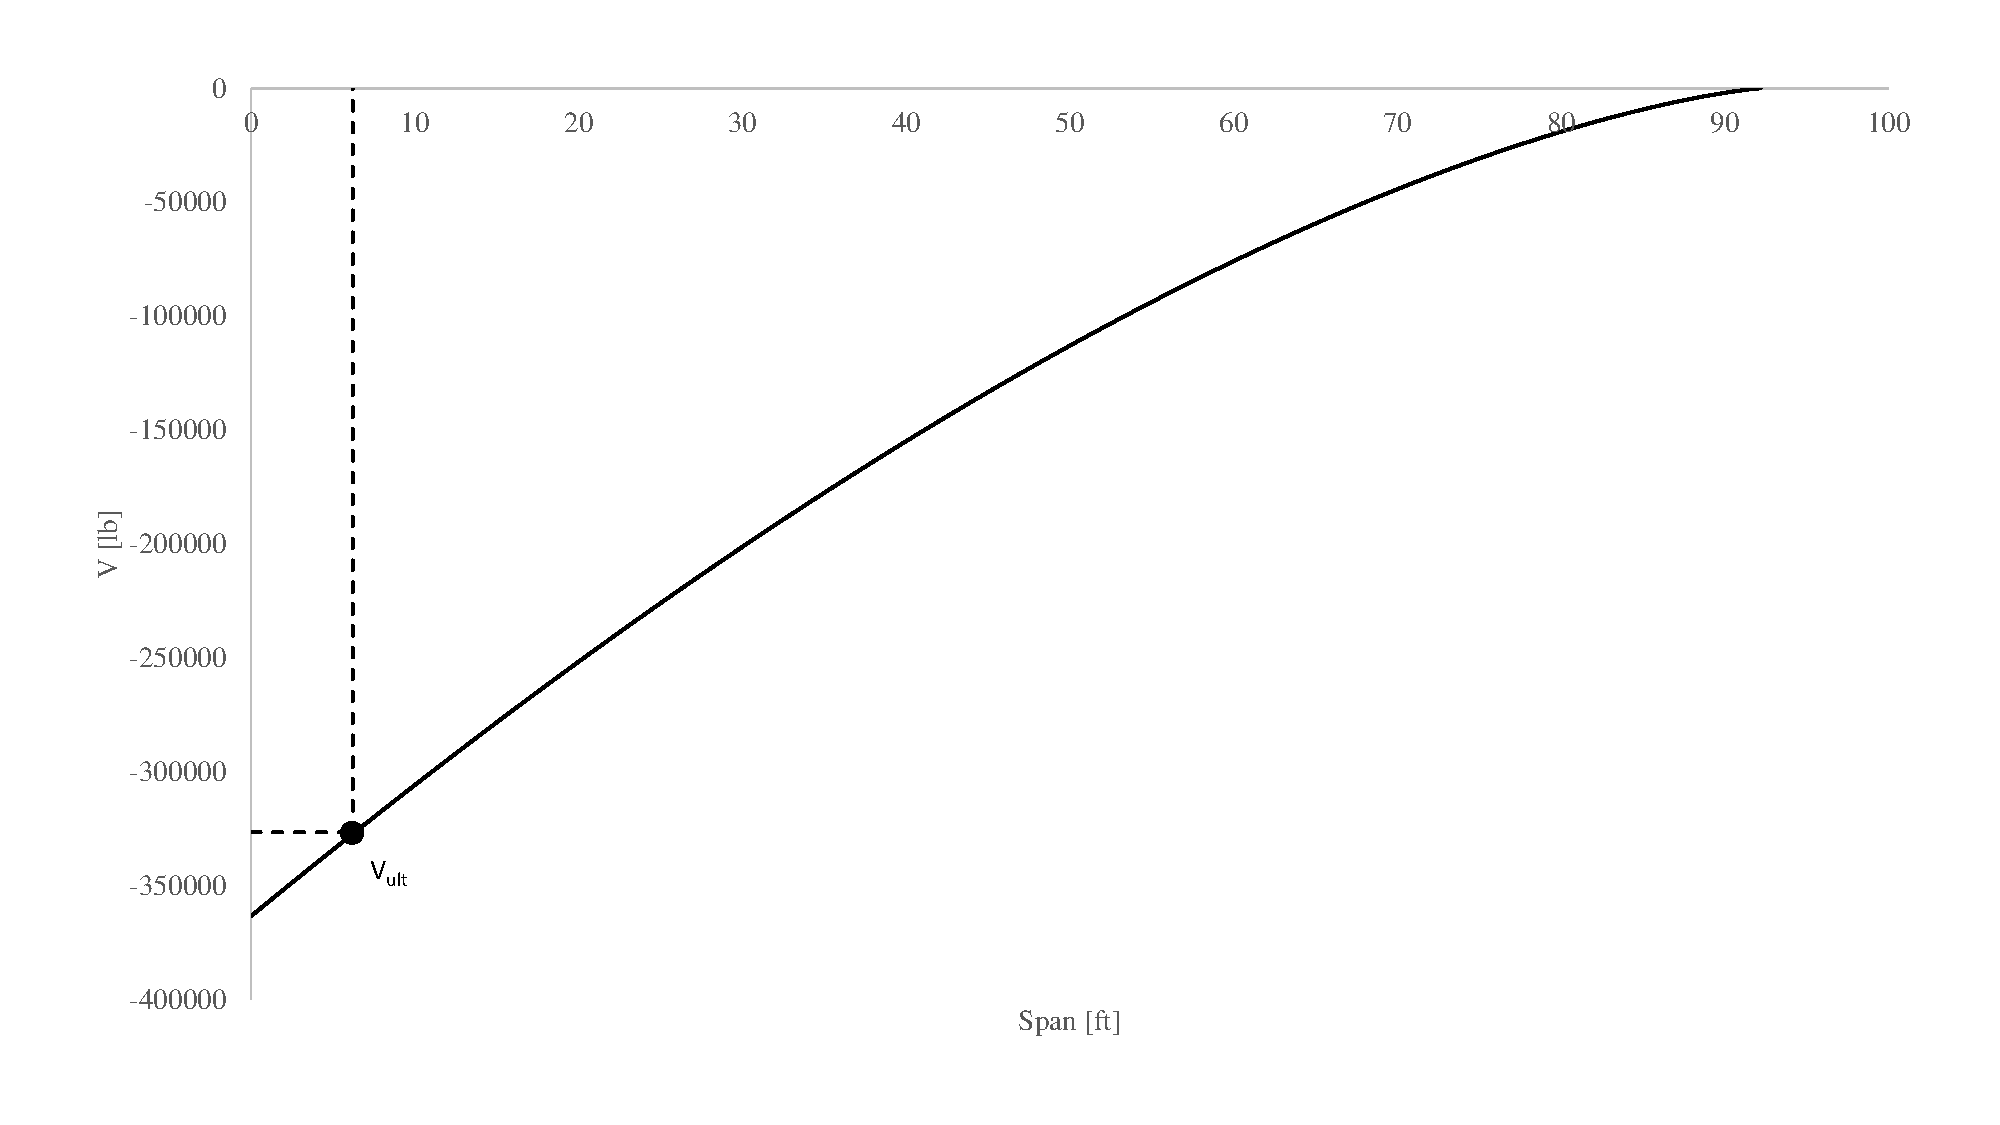
\includegraphics[width=1.0\linewidth]{Photos/Shear.pdf}
    \caption{Shear Diagram Across the Half-span Wing}
    \label{sheardiag}
\end{figure}

\begin{figure}[H]
    \centering
    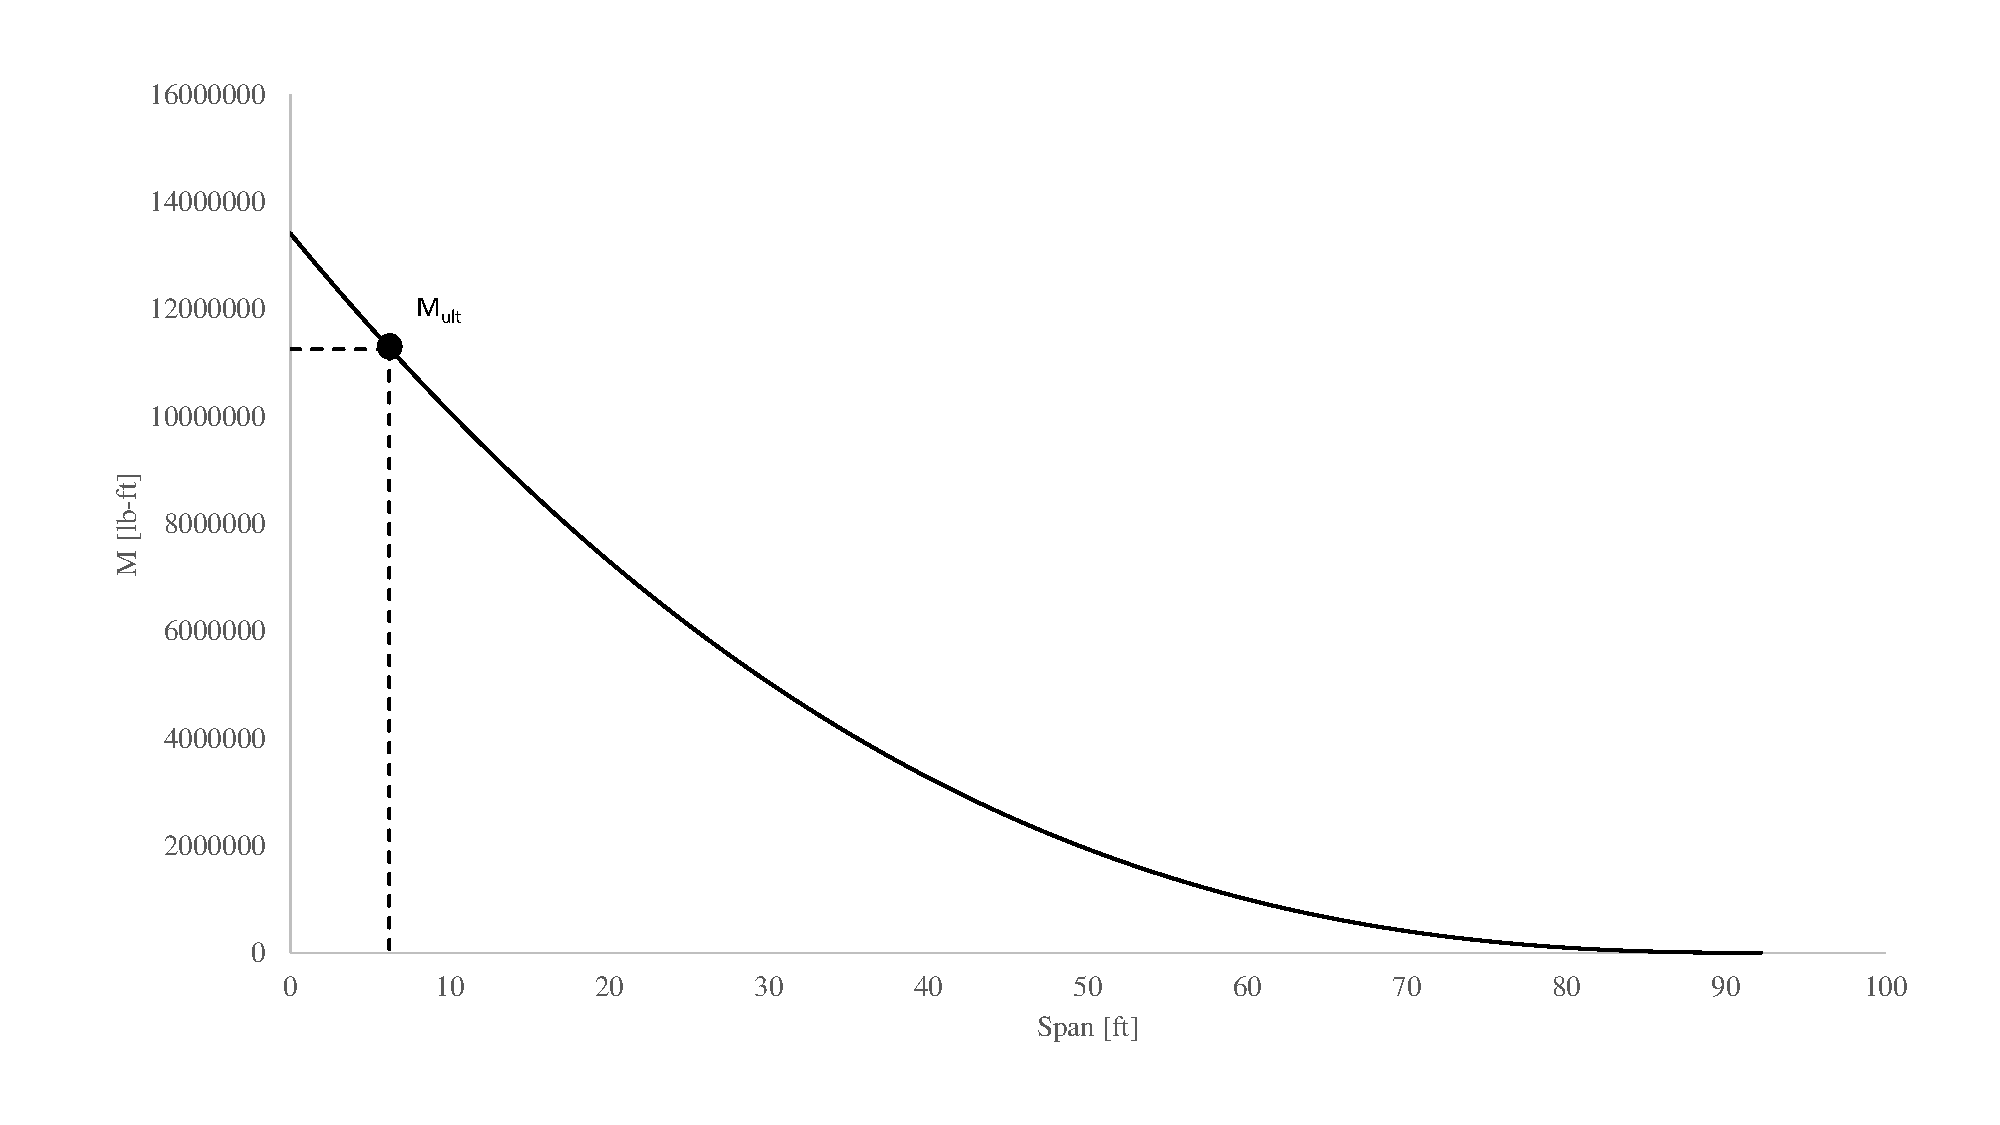
\includegraphics[width=1.0\linewidth]{Photos/Moment.pdf}
    \caption{Bending Moment Diagram Across the Half-span Wing}
    \label{momentdiag}
\end{figure}

\clearpage
Finally, the ultimate shear load and ultimate bending moment need to be determined. These can be estimated by estimating the distance from the center of the fuselage to the location of the wing attachment to the fuselage. This wing attachment location was estimated to be 6.2 ft from the center of the fuselage. This location is where the wing will feel the ultimate shear load and bending moment, which were estimated to be -327,000 lb and 11,276,000 lb-ft, respectively. These are represented in Figures \ref{sheardiag} and \ref{momentdiag} as black dots. 

\subsubsection{Load Paths}
As the wing is experiencing aerodynamic loads, those loads are transferred onto the structure of the aircraft. From the Schrenk's approximation of the lift distribution across the wing, the load then gets transferred onto the wing panels. From there, the loading transfers onto the spars, which lead to the wing box. Then, from the wing box, the loading goes into the fuselage, where the maximum loading occurs. The ribs on the wing absorb the shear produced by the bending moment from the lift distribution. Additionally, the engine also produces a load onto the wing. This loading follows a similar path, except it moves into the pylon first, then into the wing panels. From there, the load transfers into the spars, which moves into the wing box, and finally into the fuselage. Figure \ref{loadpath} shows a diagram of the load paths across half the aircraft, since it will be symmetric along the center line of the fuselage. 

\begin{figure}[H]
    \centering
    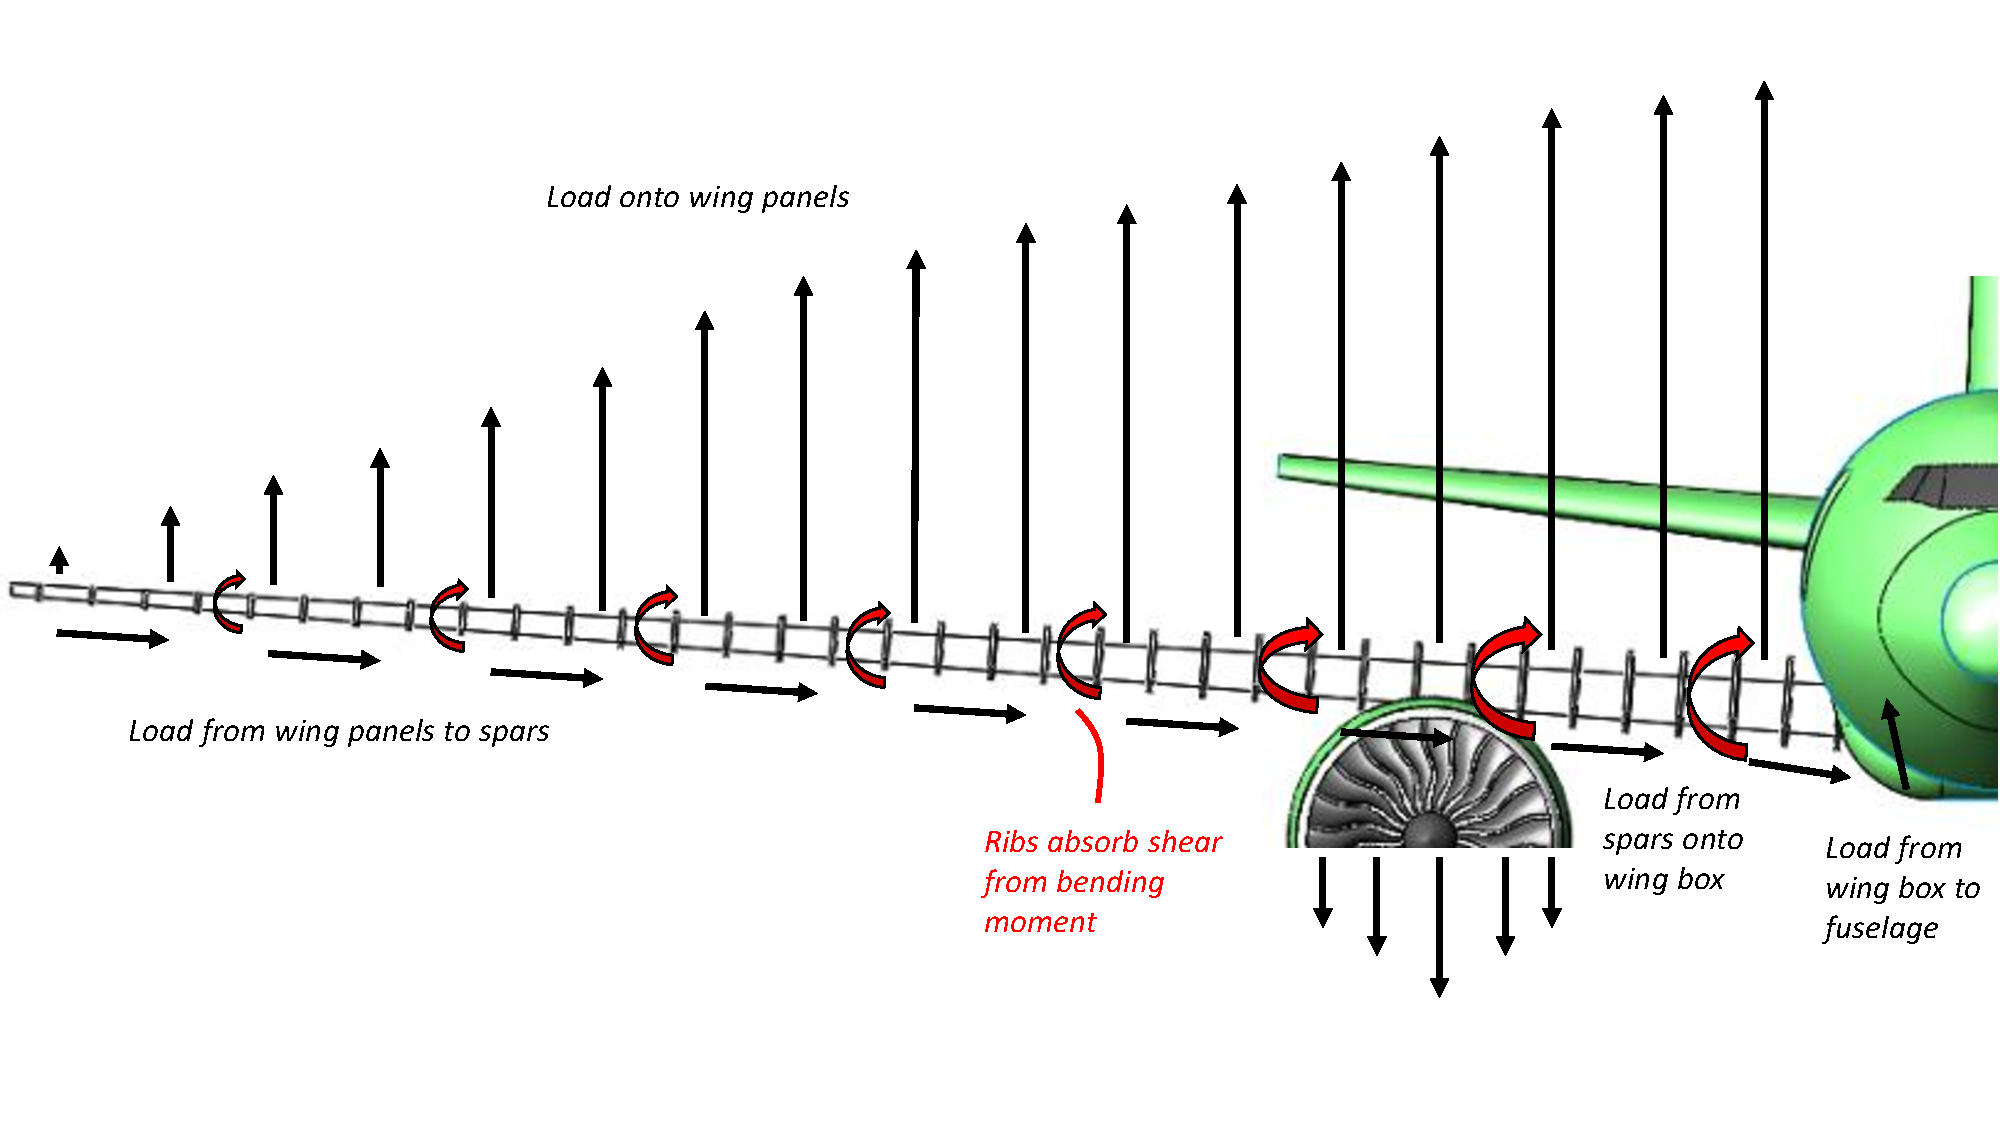
\includegraphics[width=1.0\linewidth]{Photos/Load_Path.pdf}
    \caption{Load Path of the Lift Distribution, Engine Weight, and Pressurization}
    \label{loadpath}
\end{figure}

\newpage
Furthermore, the aircraft will experience pressurization loads during cruise flight. Accoriding to the RFP \cite{RFP}, the aircraft will need to be pressurized to 8,000 ft pressure altitude above that altitude. Thus, there will be a pressure differential, specifically a max differential at the point where the aircraft is at its highest altitude. Since SAM Mk. 1 will be starting at a cruise altitude of 37,000 and end at 41,000 ft, the last altitude height will carry the highest pressure differential in the aircraft. The fuselage will feel this differential as displayed in the load path diagram in Figure \ref{loadpath}.
Table \ref{tab:pres} displays the pressures the aircraft will be pressurized to, the pressure at 41,000 ft altitude, and the differential between both those values. 

\begin{table}[!h]
    \centering
    \caption{Pressure Differential}
    \begin{tabular}{|c|c|c|c|}\toprule 
     & \textbf{8,000 ft (Cabin)} & \textbf{41,000 ft} & \textbf{Difference} \\ \hline 
    \textbf{Pressure [psi]} & 10.92 & 2.59 & 8.32 \\ 
    \bottomrule
    \end{tabular}
    \label{tab:pres}
\end{table}

With this pressure difference comes a stress on the fuselage skin. This pressure differential results in a hoop stress that the fuselage feels. To calculate this stress, the hoop stress equation for a thin-walled pressure vessel was used, along with a skin thickness of 0.045 in. Table \ref{hoopstrs} displays the hoop stress felt by the fuselage.

\begin{table}[!h]
    \centering
    \caption{Pressure Differential}
    \begin{tabular}{|c|}\toprule 
    \textbf{Hoop Stress (8,000 ft) [psi]} \\ \hline
    26,200 \\ 
    \bottomrule
    \end{tabular}
    \label{hoopstrs}
\end{table}

\subsubsection{Load Cases of Interest}
\label{lcoi}
There are several cases of loads that apply to the aircraft, with some load cases being more significant than others. The highest loads experienced by the aircraft come from maneuver and gust loads, as described in the V-n diagram in Section \ref{subvn}. An example of a maneuvering load is turning, where the aircraft needs to be able to handle the amount of gs experienced when suddenly changing directions. The next important load case is during cruise flight. In particular, this segment of the mission experiences pressurization loads. This is significant because as altitude increases, the pressure outside the cabin will decrease while the inside cabin pressure stays at a constant value. This will create some bulging of the fuselage, which will put high stresses on the aircraft. Moreover, in cruise flight and climb and descent, the aircraft will experience aerodynamic loads, as described in Section \ref{winlod}. This will put stresses across the span of the wing, which will lead to high stress at the interface of the wing and fuselage. Another load case of interest corresponds to the aircraft landing. This puts stresses not only on the landing gears, but this transfers to the fuselage and wing of the aircraft. Finally, the taxi segment of the mission profile experiences stresses on the aircraft. While the aircraft is not actually flying at this stage, it still experiences loads due to any turns or bumps it passes. While these are not as significant as maneuvering and gust loads, these loads are still an important aspect to take into consideration when analyzing the loads experienced by the aircraft.



% \textcolor{red}{
% \begin{itemize}
%     \item Discuss any analysis supporting the sizing analysis.
%     \item Discuss future work.
%     \item AIAA: A V -n diagram for the aircraft with identification of necessary aircraft velocities and design load factors.
%     Required gust loads are specified in 14 Code of Federal Regulations (CFR) Part 25
%     \item AIAA: Materials selection for main structural groups and general structural design, including layout of primary airframe structure as well as the strength capability of the structure
%     and how that compares to what is required at the ultimate load limits of the aircraft.  The maximum dive speed shall be specified.
% \end{itemize}}
\subsection{Landing Gear}
\label{section: Landing Gear}
\subsubsection{Configuration}

Given the main configuration stated above, the landing gear was sized such that the main struts and nose struts were able to carry the maximum dynamic and static loads, defined in Raymer.\cite{raymer}. The primary Oleo cylinder for the main landing gear is sized to be 16 inches in diameter, whereas the front Oleo strut cylinder is sized to be 10 inches in diameter. The height and longitudinal placement of the landing gear was primarily sized given the clearance angle of \~25 degrees at take off and the maximum static and dynamic loads seen by each gear. \cite{raymer} In Fig. \ref{fig:landing_gear_CG}, it can be seen that main landing gear is placed aft of the MTOW CG limit, labelled as "AFT" in the figure. Given this, it can be assumed that the aircraft will be stable on the ground at MTOW.

\begin{figure}[!h]
    \centering
    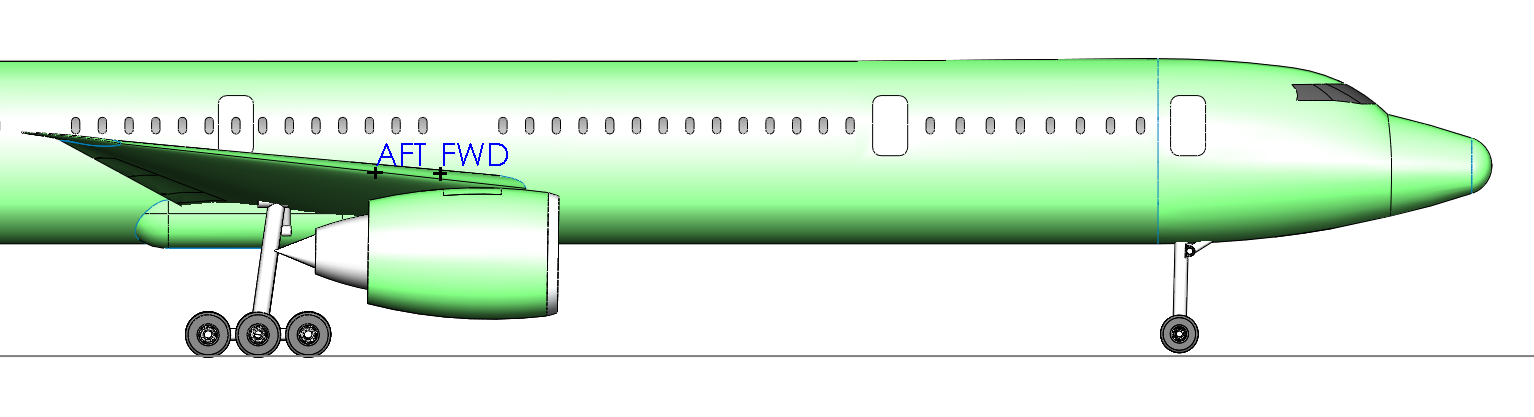
\includegraphics[width=\linewidth]{Photos/landinggear/LG Close Side View with CG.PNG}
    \caption{SAM Mk1 Landing Gear in Relation to CG Limits}
    \label{fig:landing_gear_CG}
\end{figure}


\subsubsection{Kinematics}
The landing gear must also be designed in such a way which allows seamless stowage into the belly of the aircraft. In Figs. \ref{fig:main_landing_kin} and \ref{fig:nose_landing_kin}, the kinematics of the main and nose landing gear are shown. As seen, both the main and nose landing gear stow into the aircraft without interference.

\begin{figure}[!h]
    \centering
    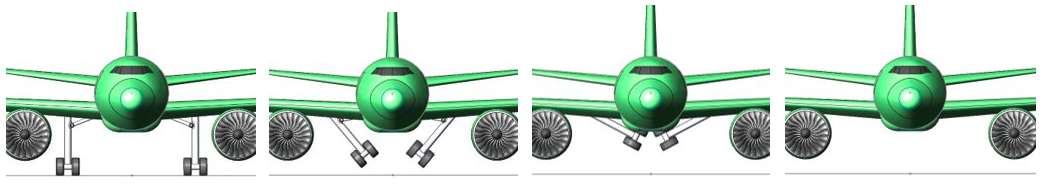
\includegraphics[width=\linewidth]{Photos/landinggear/Main Gear Kinematics.PNG}
    \caption{SAM Mk. I Main Landing Gear Kinematics}
    \label{fig:main_landing_kin}
\end{figure}

\begin{figure}[!h]
    \centering
    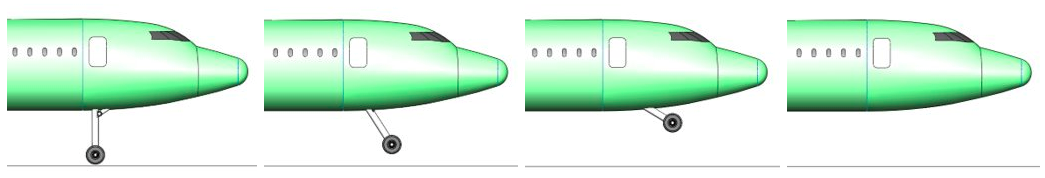
\includegraphics[width=\linewidth]{Photos/landinggear/Nose Gear Kinematics.PNG}
    \caption{SAM Mk. I Nose Landing Gear Kinematics}
    \label{fig:nose_landing_kin}
\end{figure}


\subsubsection{Tire Selection (JJ)}
With the SAM Mark I falling within the weight and size boundaries of established commercial aircraft, designing to utilize tires already available from known manufacturers saves cost and time, and also mitigates the threat of setbacks due to developmental overruns from the manufacturer. Bridgestone was selected as a launch supplier for both the nose (two) and main (twelve) tires using existing tires from their APR line first introduced for the Boeing 777-300ER/200LR in 2004 \cite{bridgestonetire}.  Their listed specifications, as published by Bridgestone \cite{bridgestonetire}, are below in Table \ref{tab:tires}.  Per FAA FAR Part §25.733 \cite{cfr}, the tires will be filled with dry nitrogen to mitigate issues caused by dioxygen, a powerful oxidizer, at high heats as well as moisture, both found in ambient air. 

\begin{table}[!h]
    \centering
        \caption{Tire Specifications}
    \begin{tabular}{|c||c|c|>{\centering}p{.8in}|>{\centering}p{.7in}|>{\centering}p{.95in}|c|}\toprule
         & \textbf{Size} & \textbf{Ply Rating} & \textbf{Speed Rating [MPH]} & \textbf{Rated Load [lb]} & \textbf{Average Weight [lb]} & \textbf{Model} \\\hline \hline
         \textbf{Main} & 52x21.0R22 & 36 & 235 & 66,500 & 266 & APR07700 \\ \hline
         \textbf{Nose} & 43x17.5R17 & 32 & 235 & 44,500 & 156 & APR06600 \\ \hline
    \end{tabular}
    \label{tab:tires}
\end{table}


% \textcolor{red}{
% \begin{itemize}
%     \item Discuss landing gear sizing, tire sizing, loads, and retraction system.
%     \item Include CAD drawings with landing gear extended and stowed.
%     \item Discuss pressurization (if used).
%     \item Consider merging into Structures as a sub section
% \end{itemize}}

\clearpage
\section{Mass Properties (\textit{CE})}
\label{section: Mass Properties}
\subsection{Comparison Analysis}
\label{subsection: comparison}
Given the preliminary geometry of the aircraft, the mass properties of the aircraft's sections were calculated and tabulated in Table \ref{tab:mass_props}. Equations used and analyzed came from Raymer \cite{raymer} and Roskam Part V \cite{roskam_5}, class II analysis for traditional construction of aircraft. To account for the use of composites in the wing, horizontal and vertical stabilizers, a correction factor of 0.8* was applied, the weight savings quoted by Boeing Commercial Aircraft for composite aircraft structure over aluminum structure, was applied to estimations for the aircraft's lifting surfaces \cite{bcacomposite}.  Finally, an actual weight was chosen by either an average or closest value to the estimated weight from the seed aircraft (777-200) given the seed inputs.

\begin{table}[!h]
\centering
\caption{Independent Mass Estimations of SAM Mk I}
\begin{tabular}{|c||c|c|c|c| }
\toprule
\multicolumn{1}{|c||}{\textbf{Description}} & \multicolumn{1}{c|}{\textbf{Raymer Weight}} &  
 \textbf{Roskam Weight} & \textbf{Design Weight} & \textbf{Equation Used} \\ \hline \hline 
Wing & 32,000* & 31,600* & 31,600* & Roskam 5.6  \cite{roskam_5} \\ \hline
Fuselage & 61,600 & 41,900 & 41,900 & Roskam 5.27  \cite{roskam_5} \\ \hline
Horizontal Stabilizer & 6,000* & 9,800* & 9,900* & Roskam 5.19 \cite{roskam_5} \\ \hline
Vertical Stabilizer & 2,500* & 3,900* & 3,900* & Roskam 5.20 \cite{roskam_5} \\ \hline
Main Landing Gear & 4,100 & 11,900 & 11,900 & Roskam 5.42  \cite{roskam_5} \\ \hline
Nose Landing Gear & 450 &2,400 & 2,400 & Roskam 5.42  \cite{roskam_5} \\ \hline
Fixed Equipment & 55,000 & 65,000 & 60,000 & Roskam V Pgs. 97-111 \cite{roskam_5}  \\
& & & & \& Raymer Pgs. 575-576 \cite{raymer} \\ \hline
Engine Weight (per) &  \multicolumn{4}{|c|}{19,316}   \\ \hline
Baggage Weight & \multicolumn{4}{|c|}{12,300 (30 lb/occupant) }  \\ \hline
Payload Weight & \multicolumn{4}{|c|}{82,000 (200 lb/occupant) }  \\ \hline
Fuel Weight & \multicolumn{4}{|c|}{146,860, (6.1 lb/gal) }  \\ \hline \hline
\textbf{Empty Weight} & 160,326 & 217,371 & \textbf{216,200} & -\\ \hline
\textbf{MTOW} & 364,626 & 421,671 & \textbf{443,800}  & - \\ \hline
\textbf{MZFW} & 242,326 & 299,371 & \textbf{310,500}  & - \\ \hline
\textbf{MLW} & 168,165 & 219,197 & \textbf{388,400} & - \\
\bottomrule
\end{tabular}
\label{tab:mass_props}
\end{table}
\FloatBarrier

It was found that Roskam, specifically the General Dynamics and Torenbeek methods, estimated the weight of the structure and landing gear with a smaller percentage of error when calculating MTOW for the 777-200 and other seed aircraft than the Raymer equations. Because of the higher fidelity of the structure and landing gear weight given by Roskam, Roskam class II was utilized for those section. Fixed equipment, which consists of systems, avionics, fuel systems, and other miscellaneous necessities of the aircraft, was estimated using the average between Raymer and Roskam build-ups. The engine, the GE90-115B, weight is a direct value from the manufacturer.\cite{roskam_5}\cite{raymer}

\newpage
\subsection{Center of Gravity}
The center of gravity (CG) of the aircraft was also estimated using the class II estimation methods found in Roskam Part V and Raymer.\cite{roskam_5}\cite{raymer} In Table \ref{tab:cg}, the CG locations of each major component is tabulated. Note that the locations in the table are referenced from the aircraft's "master coordinate system", which is located forward and below the nosecone of the aircraft seen in Fig. \ref{fig:master_coord_def}.

\begin{table}[!h]
\centering
\caption{CG Locations of Primary Structures and Systems}
\begin{tabular}{|c||c|c|c|c|c|}
\hline
\textbf{}   & \textbf{X Location (ft)} & \textbf{$X_{CG}$ (ft-lb)} & \textbf{Z Location (ft)} & \textbf{$Z_{CG}$ (ft-lb)} & \textbf{Eq $\#$ or Pg. \#} \\ \hline \hline
\textbf{Wing}            & -135.2      & -4273678   & -33.8       & -1068791   & Roskam Table 8.1        \\ \hline
\textbf{Fuselage}        & -128.3      & -5377027   & -38.0       & -1592200   & Roskam Table 8.1        \\ \hline
\textbf{H-Stab}          & -235.4      & -2330049   & -39.9       & -395208    & Roskam Table 8.1        \\ \hline
\textbf{V-Stab}          & -228.7      & -891903    & -56.2       & -219206    & Roskam Table 8.1        \\ \hline
\textbf{Main Gear (ext)} & -23.3       & -277627    & -26.3       & -313366    & Roskam Table 8.1        \\ \hline
\textbf{Nose Gear (ext)} & -23.3       & -55992     & -26.3       & -63200     & Roskam Table 8.1        \\ \hline
\textbf{Engines}         & -131.6      & -5092275   & -27.7       & -1070442   & \begin{tabular}[c]{@{}c@{}}Assumed CG at \\ center of engine\end{tabular}   \\ \hline
\textbf{Fixed Equipment} & -123.3      & -7395000   & -38.0       & -2280000   & \begin{tabular}[c]{@{}c@{}}Assumed CG at \\ center of fuselage\end{tabular} \\ \hline
\textbf{Fuel System}     & -123.3      & -110925    & -38.0       & -34200     & \begin{tabular}[c]{@{}c@{}}Assumed CG at \\ center of fuselage\end{tabular} \\ \hline
\textbf{Nacelle}         & -128.7      & -1923566   & -27.7       & -413517    & Roskam Table 8.1        \\ \hline
\textbf{Full Fuel}       & -151.6      & -17277041  & -36.8       & -4197185   & Roskam 8.1              \\ \hline
\textbf{Reserve Fuel}    & -165.8      & -3199843   & -33.8       & -652774    & \begin{tabular}[c]{@{}c@{}}Assumed behind \\ wingbox\end{tabular}           \\ \hline
\textbf{Payload}         & -133.3      & -10926500  & -38.0       & -3116000   & \begin{tabular}[c]{@{}c@{}}Assumed CG at \\ center of fuselage\end{tabular} \\ \hline
\textbf{Baggage}         & -133.3      & -1638975   & -38.0       & -467400    & \begin{tabular}[c]{@{}c@{}}Assumed CG at \\ center of fuselage\end{tabular} \\ \hline
\end{tabular}
\label{tab:cg}
\end{table}

\begin{figure}[!h]
    \centering
    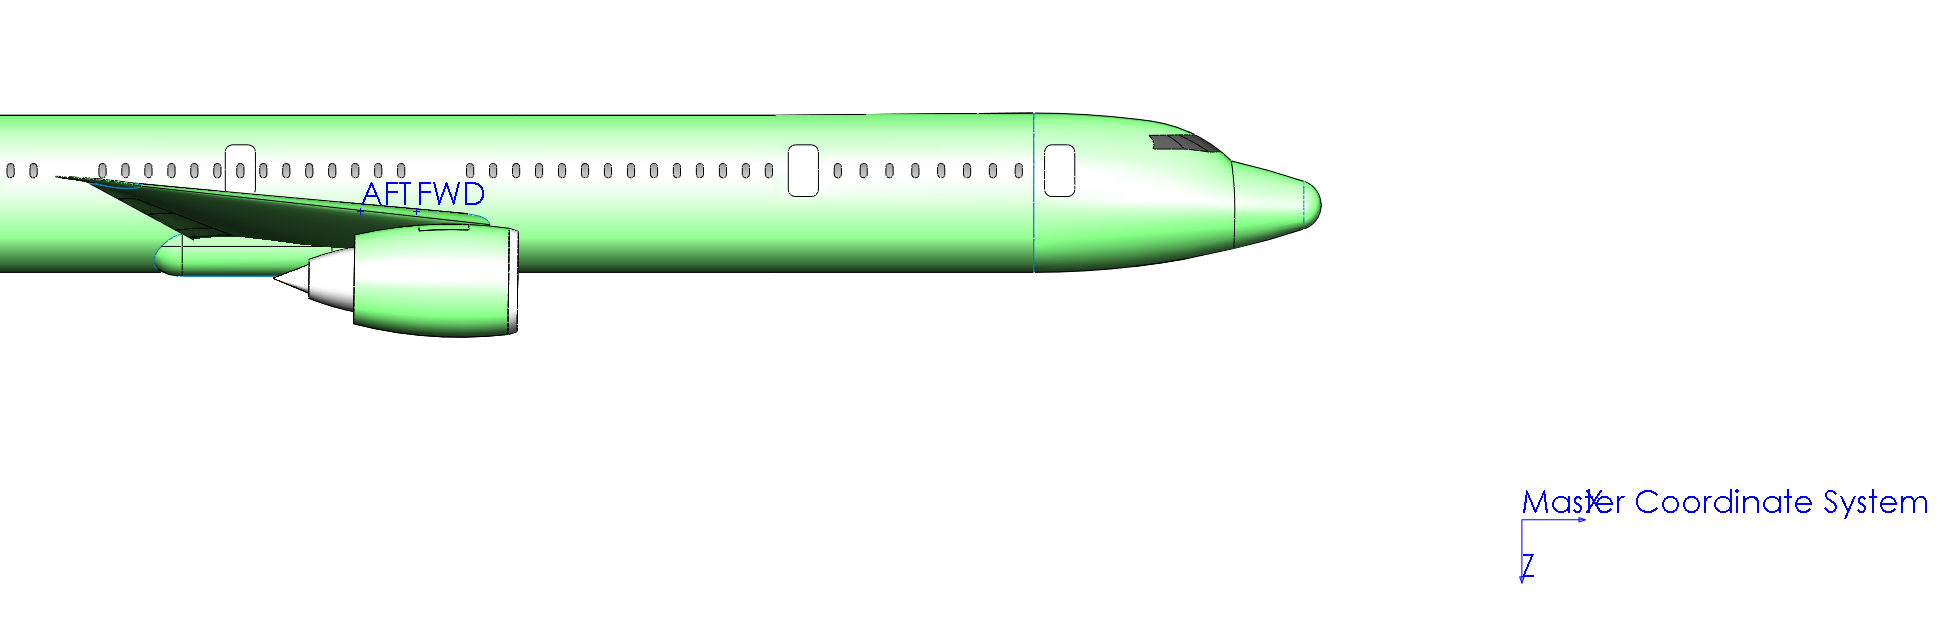
\includegraphics[width=\linewidth]{Photos/massprops/CG locations close.PNG}
    \caption{Definition of the Aircraft Coordinate System}
    \label{fig:master_coord_def}
\end{figure}
\FloatBarrier

The location of the CG limit defined by the MTOW condition and the Empty Weight condition is also depicted in Fig. \ref{fig:master_coord_def}, and tabulated in Table \ref{tab:cg}.

\begin{table}[!h]
\centering
\caption{Location of CG limits at Different Load Cases}
\begin{tabular}{|c||c|c|c|}
\hline
 & \textbf{MTOW} & \textbf{EMPTY WEIGHT} & \textbf{MAX ZERO FUEL WEIGHT} \\ \hline \hline
\textbf{X from Coordinate System (ft)} & -136.9 & -128.3 & -129.8 \\ \hline
\textbf{Z from Coordinate System (ft)} & -35.8 & -34.5 & -35.5 \\ \hline
\end{tabular}
\end{table}

\subsection{Effect of Material Composition of Center of Gravity and Weight of Aircraft}
The effect of different structure material composition was studied to see the how the weight and location of the aircraft changes as different structures of the aircraft change. The three different cases: metallic, composite, and hybrid, were studied and the total weight of the aircraft at different cases is tabulated in Table \ref{tab:mas_study}.

\begin{table}[!h]
\caption{Trade Study of Effect of Material Composition}
\label{tab:mas_study}
\begin{tabular}{|c||c|c|c|c|c|}
\hline
 & \textbf{Metallic (lb)} & \textbf{Composite (lb)} & \textbf{Hybrid (lb)} & \textbf{Delta Metallic} & \textbf{Delta Composite} \\ \hline \hline
\textbf{Empty Weight} & 227500 & 207900 & 216200 & 5.23\% & -3.84\% \\ \hline
\textbf{MTOW} & 455100 & 435500 & 443800 & 2.55\% & -1.87\% \\ \hline
\textbf{Max Zero Fuel Weight} & 321800 & 302200 & 310500 & 3.64\% & -2.67\% \\ \hline
\textbf{Max Landing Weight} & 398300 & 381100 & 388400 & 2.55\% & -1.88\% \\ \hline
\textbf{Landing Weight} & 341100 & 321500 & 329800 & 3.43\% & -2.52\% \\ \hline
\end{tabular}
\end{table}

It can be noted that the metallic structure is heavier than the hybrid structure, and the composite structure is lighter. These calculations are using the assumptions made earlier in Table \ref{tab:mass_props}.

\subsection{Center of Gravity Envelope}
When determining the stability of the aircraft, an envelope which contains the location of the center of gravity in relation to the MAC during loading of the payload, baggage, and fuel must be created. In Fig. \ref{fig:cg_envelope}, the envelope of the center of gravity of the SAM Mk. I is depicted.

\begin{figure}[!h]
    \centering
    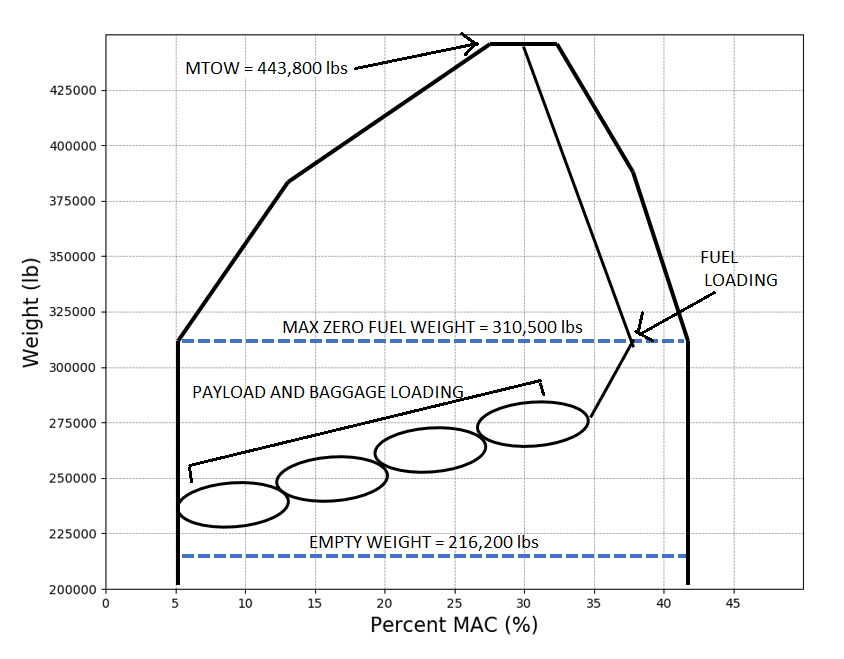
\includegraphics[width=\linewidth]{Photos/massprops/CG Envelope.PNG}
    \caption{Center of Gravity Envelope of the SAM Mk. I}
    \label{fig:cg_envelope}
\end{figure}

It can be noticed that the envelope spans from 5\% to 42\% MAC, which is in the range of the stability of the aircraft given the location of the landing gear, seen in Section \ref{section: Landing Gear}.
\newpage %may be able to delete as the document grows.  Here to put E future work beloew cg envelope pictures
\subsection{Future Work}
Future work may include using the CAD model to estimate the CG, moments of inertia, and overall mass of the aircraft once all sizing and material assignment is completed. \hl{hide or delete, state CAD CG, I, etc etc}


\clearpage
% \textcolor{red}{
% \begin{itemize}
% \item Discuss any analysis supporting the sizing analysis.
% \begin{itemize}
% \item Mass property methods chosen for different parts of the aircraft.
% \item Estimate CG location.
% \end{itemize}
% \item Discuss future work.
% \item AIAA: Aircraft weight statement, aircraft center-of-gravity envelope reflecting payloads and fuel allocation. Establish a forward and aft center of gravity (CG) limits for safe flight. (may come later...con't on AIAA doc \href{https://www.aiaa.org/docs/default-source/uploadedfiles/education-and-careers/university-students/design-competitions/undergraduate-team-aircraft-design-competition/undergraduate-aircraft-high-capacity-short-range-transport-aircraft.pdf?sfvrsn=b6081273_0}{here}: )
% \end{itemize}}

%\clearpage
%\section{Landing Gear (\textit{CE, JJ})}
%\label{section: Landing Gear}
%\subsection{Configuration}
The aircraft will feature three sets of retractable landing gear customary of that found on similar aircraft within the aircraft featured in the trade study found in Table \ref{tab:trade_params}. Tentatively, the nose gear will be composed of two wheels, and the main gear will consist of two symmetric sets of six wheels each, three wheels in a line on each side of each set.  All of the gear will be hydraulically mounted to dampen the impact seen upon touchdown, as well as hydraulically actuated. The "tricycle" arrangement is traditionally seen due to both the stability of three on uneven surfaces as well as the weight distribution of the aircraft.  The front gear will also feature the main taxi light. Landing gear doors will most likely be utilized in order to increase performance characteristics by reducing drag. 

\subsection{Future Work -- Delete when discussed}
Future work will consist of an analysis of the load and stress placed on the landing gear during taxi, takeoff, and, most importantly, landing.  Additional consideration will be taken to ensure the landing gear and its related hydraulic systems stow within the contour of the fuselage as developed by aerodynamics. The necessary kinematics of the gear will be studied. Furthermore, brake sizing and fitment inside the wheel will be verified. The number, size, and type of wheels and number of struts needed must be finalized. Lastly, the height of the landing gear will be determined by the takeoff and flare angle, the placement of the gear, and length of the fuselage.

\subsection{Tire Selection (JJ)}
With the SAM Mark I falling within the weight and size boundaries of established commercial aircraft, designing to utilize tires already available from known manufacturers saves cost and time, and also mitigates the threat of setbacks due to developmental overruns from the manufacturer. Bridgestone was selected as a launch supplier for both the nose (two) and main (twelve) tires using existing tires from their APR line first introduced for the Boeing 777-300ER/200LR in 2004 \cite{bridgestonetire}.  Their listed specifications, as published by Bridgestone \cite{bridgestonetire}, are below in Table \ref{tab:tires}.  Per FAA FAR Part §25.733 \cite{cfr}, the tires will be filled with dry nitrogen to mitigate issues caused by dioxygen, a powerful oxidizer, at high heats as well as moisture, both found in ambient air. 

\begin{table}[!h]
    \centering
        \caption{Tire Specifications}
    \begin{tabular}{|c||c|c|c|c|c|c|}\toprule
         & \textbf{Size} & \textbf{Ply Rating} & \textbf{Speed Rating [MPH]} & \textbf{Rated Load [lb]} & \textbf{Average Weigh [lb]} & \textbf{Model} \\\hline \hline
         \textbf{Main} & 52x21.0R22 & 36 & 235 & 66,500 & 266 & APR07700 \\ \hline
         \textbf{Nose} & 43x17.5R17 & 32 & 235 & 44,500 & 156 & APR06600 \\ \hline
    \end{tabular}
    \label{tab:tires}
\end{table}


% \textcolor{red}{
% \begin{itemize}
%     \item Discuss landing gear sizing, tire sizing, loads, and retraction system.
%     \item Include CAD drawings with landing gear extended and stowed.
%     \item Discuss pressurization (if used).
%     \item Consider merging into Structures as a sub section
% \end{itemize}}

\clearpage
\section{Auxiliary Systems (\textit{KP})}
\label{section: Systems}
The SAM Mark I includes every system that is compulsory in order to satisfy the given requirements meanwhile optimizing the aircraft's safety, and comfort. The aircraft's main systems are flight controls, deicing systems, engine control systems, environmental control systems, fuel systems, battery systems, along with an electrical and hydraulic system. These systems were chosen to provide the aircraft with the latest system technologies that are not present in older aircraft, and to provide safe flights. Due to the fact that the SAM Mark I is a large aircraft, each system has a redundancy factor built into it in case of a malfunction of any part. 

\subsection{Flight Controls}
The SAM Mark I will utilize a Fly-By-Wire (FBW) flight control system in order to help reduce overall airframe weight and increase the ease of maintenance and manufacturing. A conventional primary flight control system incorporates hydraulic actuators and control valves, that are controlled by pilot driven cables \cite{fbw}. Due to the long cable runs, however, this conventional system adds to the overall system weight and increases the amount of total components in the system, which is why the electronic based FBW system was chosen. The FBW system relies on electronic computers that are located in the cockpit’s main flight control computer. Position transducers are attached to pilot controls which send electrical signals for the computers to convert into commands that are then communicated to the actuators \cite{fbw}. The SAM Mark I will also include a secondary electric computer in case the main flight computer breaks down or fails to send the required signals.

The primary flight controls included in the SAM Mark I are: one outboard aileron, multiple flaperons and spoilers per wing, an elevator per horizontal stabilizer wing, and a single rudder on the vertical horizontal tail. These control surfaces on the wings and tail are operated by hydraulically powered, electrically signaled actuators. Each elevator, flaperon and aileron surface will be controlled by two actuators, while the vertical tail rudder will be controlled by three. These control surfaces that will be controlled by the fly-by-wire system will improve the SAM Mark I’s system reliability and maintainability.

\begin{figure}[H]
    \centering
    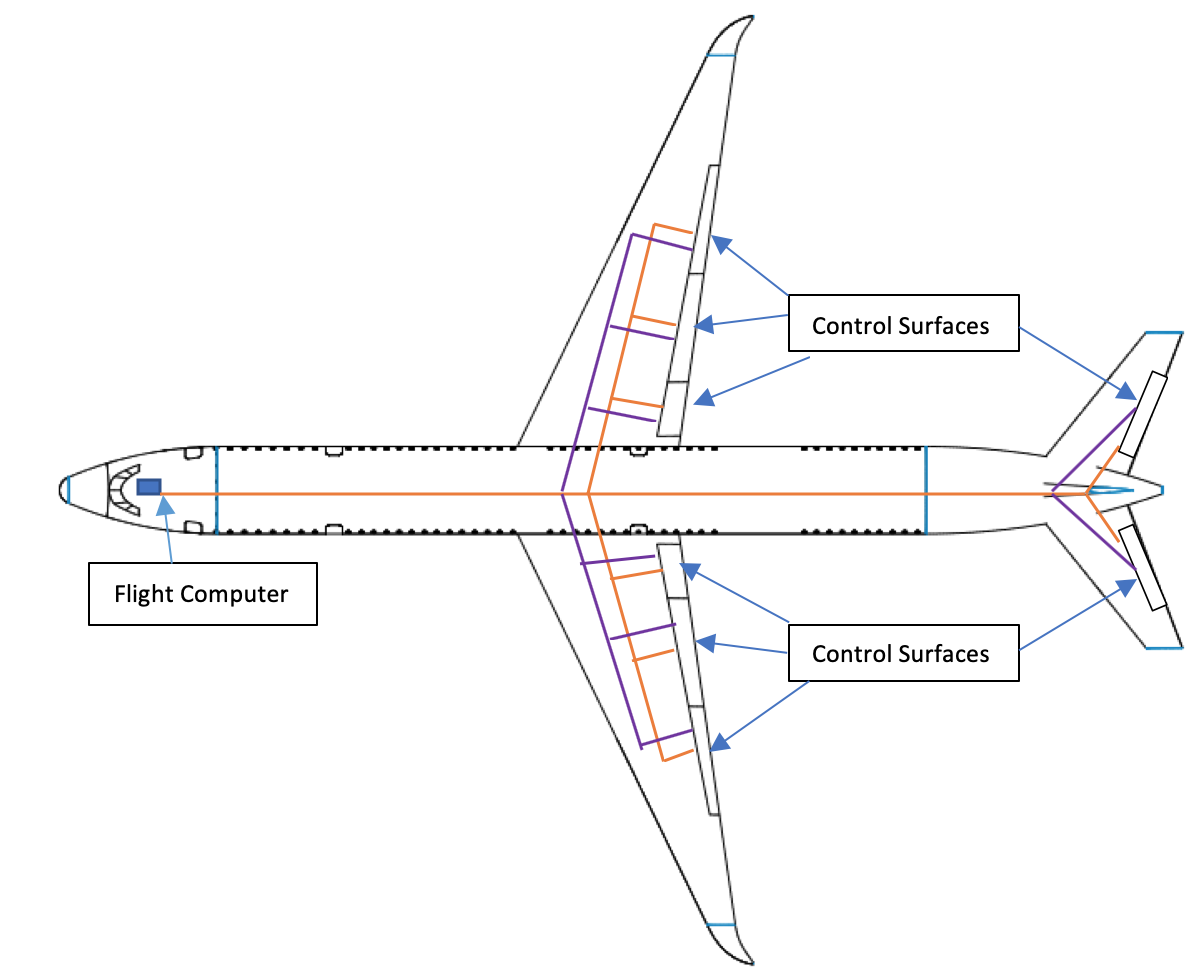
\includegraphics[width=.75\linewidth]{Photos/systems/flight_controls.png}
    \caption{Flight Controls Diagram}
    \label{flighte_controls}
\end{figure}

\subsection{Engine Controls}
The SAM Mark I will utilize a full authority digital engine control (FADEC), which will contain an engine control unit (ECU) and all components related to maintaining quality engine performance. The ECU's will be located on the engine's fan casing. The FADEC system was chosen because it provides the aircraft with optimum engine efficiency. The ECU within the FADEC system receives a variety of input data such as air density, engine pressure and throttle position, and after analyzing it, relays the information to FADEC which then computes the necessary engine parameters such as fuel flow, or air bleed valve position. The FADEC system is also responsible for engine starting and restarting, and during flight, applies calculated engine settings by sending electrical signals to the GE90-115B engines on the SAM Mark I. The one drawback to the FADEC system, however, is its inability to be overridden manually, meaning that the computer will have full control of all parameters of the engine. Although the automation of engine controls provides no room for human error during flight, if the FADEC system were to fail, all engines would fail as well. Therefore, a manual override will be installed in the cockpit capable of putting the aircraft's engines into manual mode in case the FADEC system experiences failure.  

\begin{figure}[H]
    \centering
    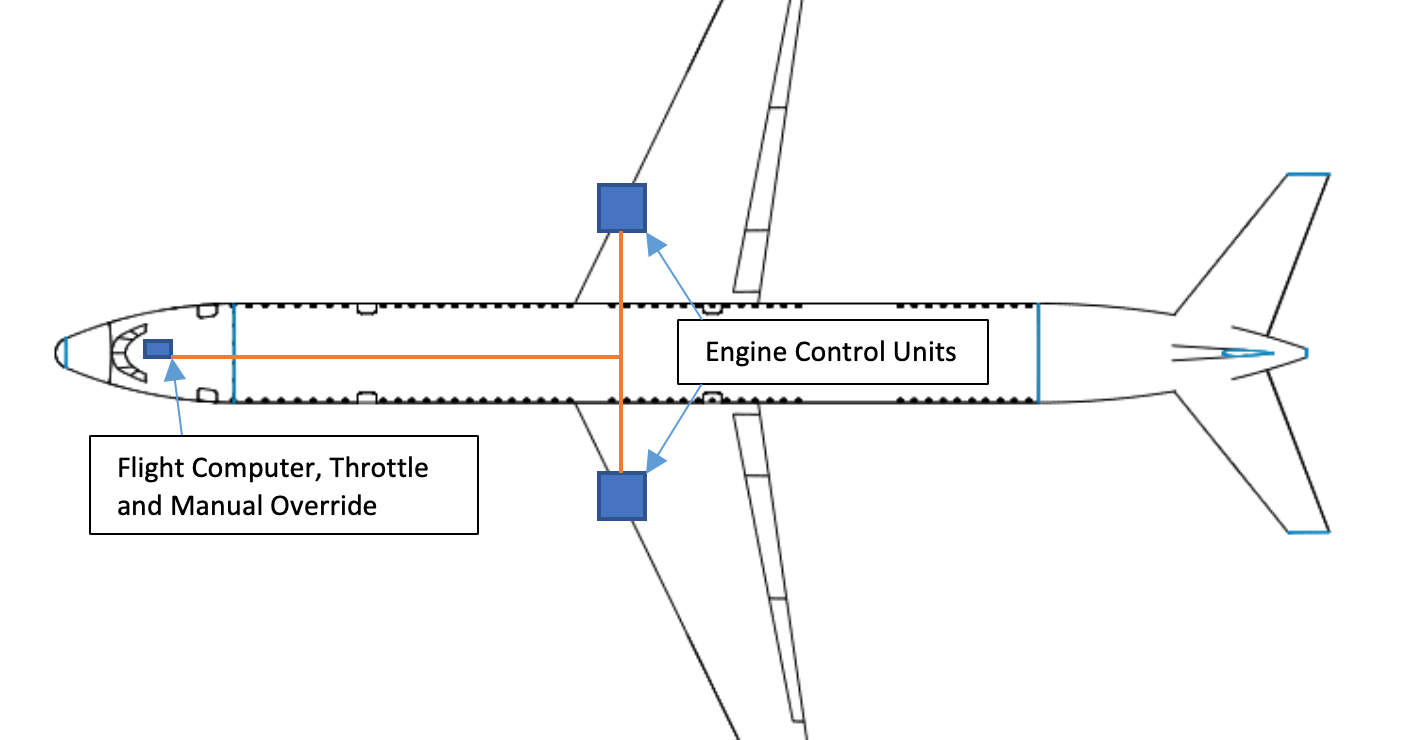
\includegraphics[width=.85\linewidth]{Photos/systems/engine_controls.png}
    \caption{Engine Controls Diagram}
    \label{engine_controls}
\end{figure}

\subsection{Fuel System}
The SAM Mark I’s fuel system is designed to effectively and safely feed the aircraft’s engines during flight. The SAM Mark I will store fuel in five tanks; two in the left wing, one center tank, and two in the right wing. Each fuel tank will contain two fuel boost pumps in order to supply the engine with fuel. This fuel system will also incorporate the use of the fuel quantity indicating system (FQIS) which is made up of ultrasonic sensors throughout the tanks. These sensors send signals to a processor which calculates the volume, density, and mass of the fuel, allowing the FQIS to determine the current amount of fuel in the tank, and take control of refueling commands for each fuel tank \cite{fuel_system}. Furthermore, the FQIS system is also responsible for maintaining the correct amount of fuel in each tank, and shutting off re-fuel valves when a fuel tank reaches its designated volume. Figure \ref{fuel_tank} demonstrates the placement of fuel tanks aboard the SAM Mark I with their connected fuel lines, and the FQIS system that sends fuel data back to the cockpit.

\begin{figure}[H]
    \centering
    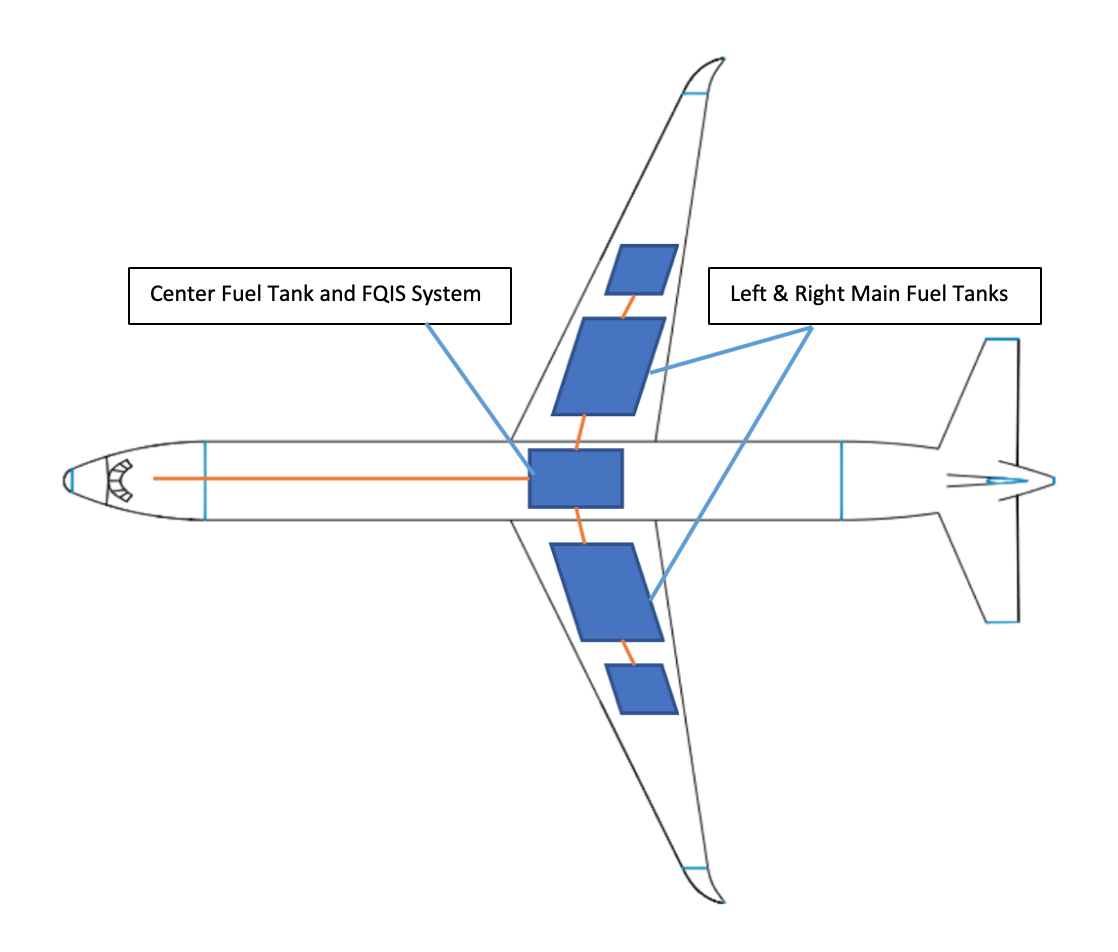
\includegraphics[width=.85\linewidth]{Photos/Fuel_tanks.png}
    \caption{Fuel System Diagram}
    \label{fuel_tank}
\end{figure}
 
\subsection{Hydraulic System}
The SAM Mark I will incorporate three hydraulic reservoirs as part of its hydraulics system. Each reservoir contains hydraulic fluid that is used to control the flap systems, actuators, brakes, landing gear, and thrust reversers. Since the SAM Mark I utilizes a fly-by-wire flight control system, the aircraft’s hydraulic system will only be used to operate control surfaces. Each reservoir will also contain an engine-driven pump (EDP) which provides hydraulic power to the system and transfers hydraulic fluid to each control surface. Each reservoir will also contain secondary motor-pumps in case of failure of the EDPs. The left and right hydraulic systems will each control their respective thrust reversers, along with each side’s respective ailerons, flaperons and elevators. The main center hydraulic system will supply pressurized hydraulic fluid in order to control the normal brake system, nose landing gear actuation and steering along with the main landing gear actuation and steering. Each hydraulic system will also have an indication system that consists of hydraulic sensors that measure and send the hydraulic pressure and temperature to the main flight computer. A detailed diagram of the SAM Mark I’s hydraulic system is presented in Figure \ref{hydrualics}. 

\begin{figure}[H]
    \centering
    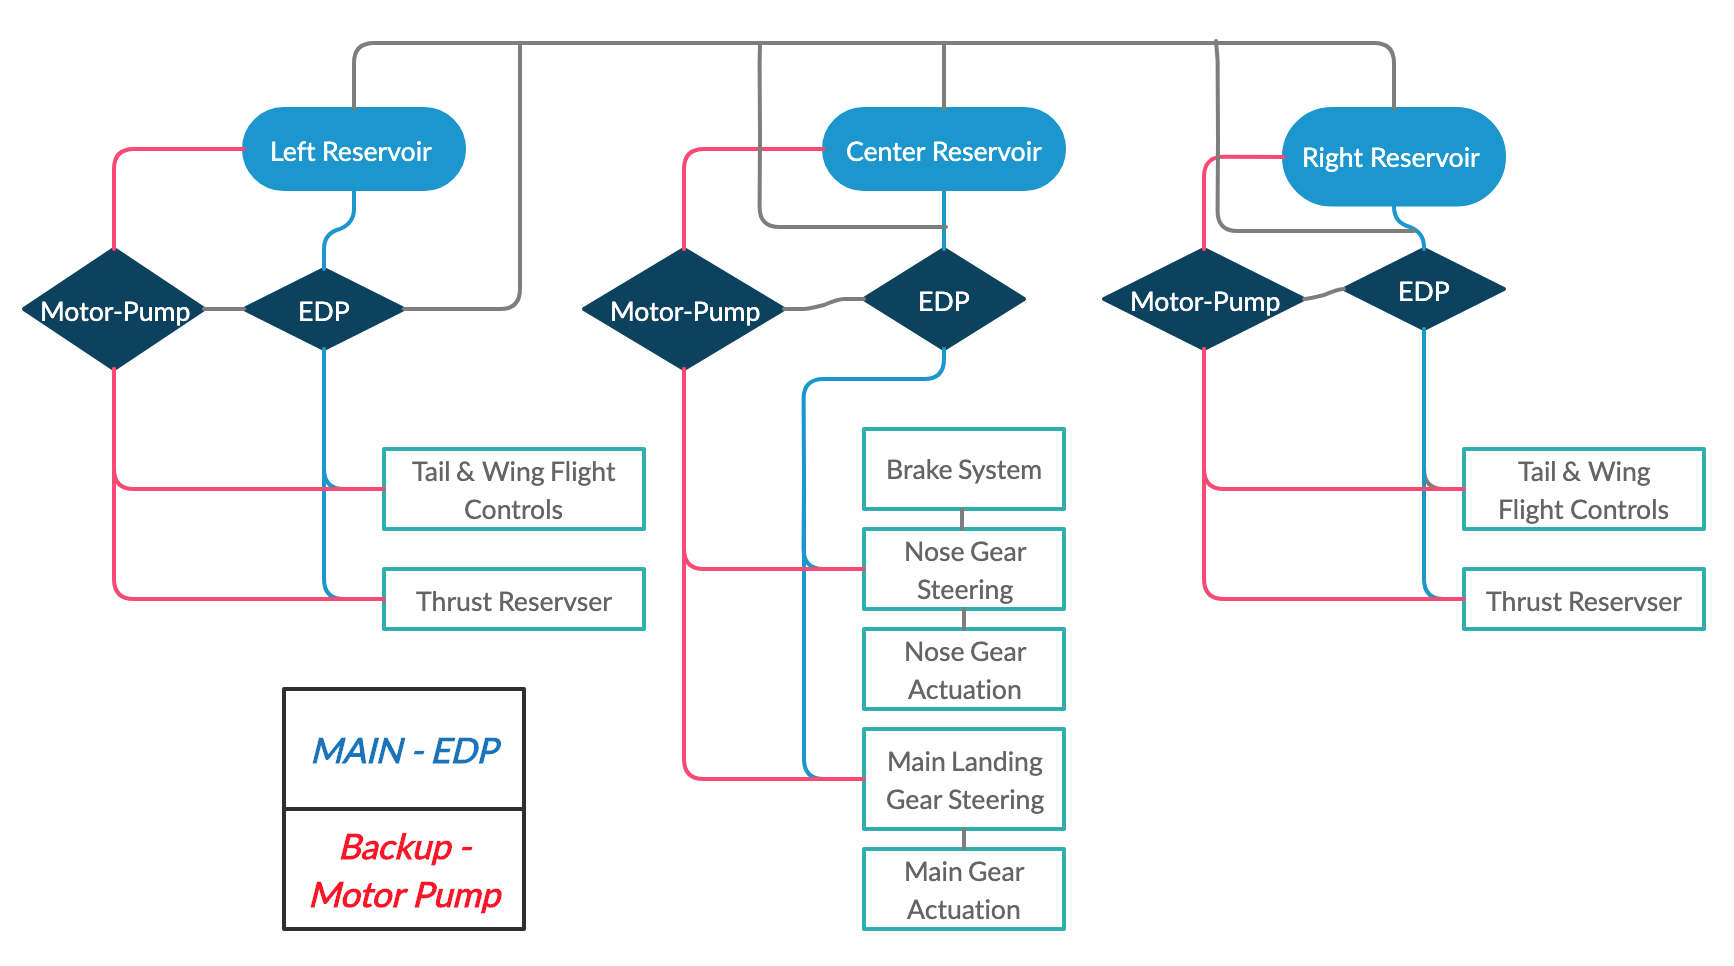
\includegraphics[width=.85\linewidth]{Photos/systems/Hydrualics.png}
    \caption{Hydraulic System Diagram}
    \label{hydrualics}
\end{figure}

\subsection{Electrical System}
Since the SAM Mark I is a large, multi-engine aircraft, it will contain two independent electrical systems: one main and one backup system. The main electrical system will consist of a generator located on each engine, a generator that is run by an auxiliary power unit (APU), three generator control units, one for each generator, and a bus power control unit. Three generators are included in this aircraft in order to share electrical loads and provide redundancy. Each of the main generators has the ability to serve either of one or both of the two main busses. The generator control units serve the purpose of regulating voltage and controlling frequency throughout the electrical systems \cite{electrical_system}. The bus power control unit is used to help the SAM Mark I distribute electrical power between the different busses on the aircraft. Two batteries will be included in the aircraft as well for powering the APU starting and backup systems. The backup electrical system also includes two engine-driven generators in case the main generators fail. Furthermore, each engine generator contains an integrated drive generator (IDG) which allows the drive to operate at constant speed \cite{electrical_system}. Each IDG also contains a generator circuit breaker which allows for the engine to operate its respective bus, and the two main busses are connected by a bus tie breaker. The bus tie breakers provide redundancy in case one of the IDGs fails, allowing the other engine IDG to power both busses. A detailed schematic of the electrical system is demonstrated in Figure \ref{electrical_system}. 

\begin{figure}[H]
    \centering
    \includegraphics[width=.75\linewidth]{Photos/systems/electrical_system.png}
    \caption{Electrical System Diagram}
    \label{electrical_system}
\end{figure}


\subsection{Pneumatic and Environmental Control System}
The SAM Mark I will incorporate an environmental control system in order to provide a comfortable flight experience for all passengers. The aircraft will contain an air conditioning and heating system that will regulate the air temperature throughout the cabin. The aircraft will contain an environmental control unit (ENCU) that will obtain compressed air from the compressor stages of the engines during flight. Inside the ENCU, the air is compressed to high pressure and temperature conditions and excess moisture is removed \cite{env_system}. After the air is conditioned, it is distributed throughout the aircraft at the desired temperature and pressure. Due to the 39,000 ft cruise flight, The SAM Mark I will also contain a pressurization system in order to set the cabin pressure to 8,000 ft pressure altitude at maximum flight altitude. The pressure will be maintained by two out-flow valves located on the aircraft, which will be opened sparingly throughout flight to prevent the fuselage from under or over pressurizing. The SAM Mark I will also contain a pneumatic bleed air system to prevent ice from forming on the aircraft’s surfaces including the wings, tail and control surfaces. The bleed air is collected from the aircraft jet engine’s compression stage, where it is then distributed to the wings, tails, and engine inlets through a series of piccolo tubes. These tubes then connect to holes located under the surfaces of the wings and control surfaces, where the hot bled air is then dispersed. This system allows the surfaces to stay above freezing temperature, and prevents ice from changing the shape of the wing, which leads to a decrease in performance.

\subsection{Emergency System(s)}
There will be a main emergency system put into place in the SAM Mark I that will focus on prevention of accidents and the protection of the passengers. The main flight computer will have the standard alarm and warning systems designated to notify the pilot of any problems the aircraft is experiencing. Fire detectors will be placed throughout the aircraft, and a fire extinguisher will be located in the cabin and rear of the aircraft. Under each seat there will be emergency life vests, and emergency oxygen masks will be stored in compartments above each passenger and crew seat. There will also be eight emergency exits on the aircraft, each immediately deploying evacuation slides in case of a crash. 

\subsection{Avionics (JJ)}
\subsubsection{Integrated Avionics System}
In order to determine which manufacturer and system provided the most holistic, yet economical avionics suite for the SAM Mark I, a comprehensive trade study was assessed on many contemporary civilian and military aircraft, as well as the updated systems offered for legacy aircraft.  Predominantly military aircraft were included because of their shared platform (tankers, reconnaissance) with older jetliners, as well as their perceived weight and cost savings at the minor expense of elegance: key for one of the most expensive aspects budget-driven design. 

\begin{table}[!h] 
    \centering
    \caption{IAS Throughout Industry}
    \begin{tabular}{ |c||c|c|c|c|c|}\toprule
    \textbf{Aircraft}  & Boeing 787 & Boeing 777 & Boeing 767/757 (Update) & Airbus A220 \\\hline 
    \textbf{IAS Provider} & General Electric & Honeywell & Rockwell Collins & Rockwell Collins  \\\hline
    \textbf{IAS System} & Common Core & AIMS & Flight2 & Pro Line Fusion \\\hline \hline
    \textbf{Aircraft}  & Lockheed C-130 & Boeing E-3 (707) & Northrop Grumman E-8 & Boeing KC-135 (707) \\\hline
    \textbf{IAS Provider} & Rockwell Collins & Rockwell Collins & Rockwell Collins & Rockwell Collins  \\\hline
    \textbf{IAS System} & Flight2 & Flight2 & Flight2 & Flight2
    \\ \bottomrule
    \end{tabular}\label{tab:ias}
\end{table}

From this study, the above (Table \ref{tab:ias}) three manufacturers and their respective integrated avionics systems (IAS) stood out as candidate systems for SAM Mark I.  To further adjudicate between, the accompanying flight control (autopilot) systems (FCS) capable of running parallel or integral to the IAS were analyzed, with Rockwell Collins' Flight2 system standing out due to the steadfast integration of a comprehensive, proven FAA-approved and certifiable FCS \cite{fcs7000pdf}.  Additionally, the military-derived simple flight deck \cite{flight2page} offered simple, rugged, ambient-air-cooled avionics \cite{flight2pdf} without the associated cost or weight of the large-format type displays found in the latest commercial aircraft \cite{flight2page}.  The IAS system will be stowed within the Electronics $\&$ Engineering (E $\&$ E bay beneath the forward galley, where there is easy access to electrical power and the cockpit.  Requiring no external cooling or other special considerations, installation should not be difficult.  Flight2 is also compatible with upgraded (all glass, large format) flight decks at carrier discretion \cite{flight2page}. 


\subsubsection{Flight Control System}
The latest RC Flight2 IAS features digital autopilot built off legacy systems which have been extensively proven through two decades of military and civilian use \cite{flight2page}.  RC's FCS-7000 is a complete FCS with a host of capabilities \cite{fcs7000pdf} including:

\begin{itemize}
    \item Fail passive, independently selectable dual autopilot computers capable of:
        \begin{itemize}
            \item IFR and VFR Flight
            \item Takeoff (selected from control yoke on ground)
            \item Go around (selected from control yoke in air)
            \item Pitch attitude hold
            \item Altitude hold (Reduced vertical separation minimum (RVSM) compliant)
            \item Altitude preselect (RVSM compliant)
            \item Flight level change (airspeed/mach/vertical speed selection)
            \item Vertical navigation (VNAV) (coupled to FMS) – RVSM compliant/altitude modes
            \item Terrain Following/Terrain Avoidance-growth
            \item Approach (Very High Frequency (VHF) Omni-Directional Range (VOR), ILS, Microwave Landing System (MLS), Global Positioning System (GPS) Localizer performance with vertical guidance (LPV))
            \item Pitch sync
        \end{itemize}
    \item Category II (Category IIIA capable) instrument landing
    \item Required Navigation Performance (RNP) RNAV 0.10, LPV (with GPS Wide Area Augmentation System (WAAS)) precision approaches
    \item FMS coupled VNAV for coupled climb, cruise, descent and approach performance/fuel optimization
    \item Gloved hand operation
    \item Flexible FD human-machine interface tailored to desired carrier systems
    \item Accommodation of a wide range of digital sensors, including display systems, as optioned by carriers
    \item FAA approved (TSO-C9c) and FAR part 23 and 25 certifiable, with design assurance level A (flight critical safety)
    \item 20-year guaranteed non-obsolescence
\end{itemize}

The decision to option an advanced FCS, significantly exceeding the AIAA RFP \cite{RFP} mandated requirements, was not taken lightly given the otherwise conservative and budget-centric nature of this aircraft. However, Toucan Aviation can not and will not discount the unequalable responsibility for the safety and well being of over 410 unique lives dependant upon the SAM Mark I for safe flight in all conditions.  Carriers will retain the option to work with RC to certify legacy Flight2-compatible autopilot systems with the FAA upon delivery.   

% \textcolor{red}{
% Discuss the follow subsystems. Each should include specifications, justifications, and
% configuration inside the aircraft as applicable. These auxiliary systems should integrate
% appropriately with other aircraft systems.
% o Flight Controls
% o Engine Controls
% o Fuel System
% o Hydraulics System
% o Electric System
% o Pneumatic System
% o Environmental Control System
% o Emergency System(s)
% o Avionics (Navigation \& Communication)}

\clearpage
\section{Cost Analysis (\textit{NZ})}    
\label{section: Cost}
\subsection{Production Cost Estimation}

The cost estimate for the Sam Mark I was done using a Development and Procurement Cost of Aircraft (DAPCA) IV Cost Model which estimated various production costs for the year 2012. These values were then subjected to inflation rates in order to gain correct estimation values for the year 2020. The DAPCA IV equations were based off a presentation made by Dr. Serkan Özgen of Middle East Technical University \cite{dapca}. The majority of the equations were based off of three dependent variables, the speed of the aircraft at cruise, the empty weight of the aircraft, and the number of units. From these three variables, it is possible to estimate the majority of the cost of an aircraft developmental program, which will be detailed in a table below.

The estimated cost of the aircraft had several uncertainties which had to be factored in and estimated, therefore it is most likely the case that the price of this aircraft is much lower than indicated. The DAPCA IV Model that was used assumes a standard material of aluminum for manufacturing, which is incorrect for the Sam Mark I material build-up. While the fuselage is metallic, the wings and stabilizers will be made of composite material, making up an estimated 43\% of the wetted area of the aircraft. According to a paper by Clifford Lester and Dr. Steven Nutt, the cost of a carbon fiber composite compared to aluminum for material and manufacturing costs is 5x \cite{compositecost}. Therefore, the manufacturing, tooling, engineering, quality, and manufacturing material cost was multiplied by a factor of 2.15 in order to account for the hybrid material design of the aircraft. The results of the DAPCA IV model are summarized in Table \ref{tab:prodcost}.

\begin{table}[!h]
    \centering
        \caption{Aircraft Cost Estimates For Varying Unit Rates}
    \begin{tabular}{|c||c|c|c|}\toprule
         & \textbf{500} & \textbf{1000} & \textbf{2000} \\\hline \hline
         \textbf{Engineering Cost} & \$ 12,373,064,000 & \$ 13,853,042,000 & \$ 15,510,044,000 \\ \hline
         \textbf{Tooling Cost} & \$ 8,092,626,000 & \$ 9,710,920,000 & \$ 11,652,826,000 \\ \hline
         \textbf{Manufacturing Cost} & \$ 40,848,815,000 & \$ 63,700,038,000 & \$ 99,334,457,000 \\ \hline
         \textbf{Quality Cost} &  \$ 8,627,232,000  & \$ 8,627,232,000 & \$ 8,627,232,000 \\ \hline
         \textbf{Development Support Cost} & \$ 971,889,000 & \$ 971,889,000 & \$ 971,889,000  \\ \hline
         \textbf{Flight Test Cost} &  \$ 23,907,000 & \$ 23,907,000 & \$ 23,907,000 \\ \hline
         \textbf{Manufacturing Materials Cost} &  \$ 25,056,881,000  &  \$ 43,596,335,000 &  \$ 75,853,032,000 \\ \hline
         \textbf{Investment Cost} & \$ 118,906,023,000 & \$ 118,906,023,000 & \$ 118,906,023,000 \\ \hline
         \textbf{Flyaway Cost} &  \$ 95,124,818,000 &  \$ 139,613,767,000 &  \$ 211,103,792,000 \\ \hline
         \textbf{Avionics Cost} &  \$ 5,620,000 & \$ 5,620,000 & \$ 5,620,000  \\ \hline
         \textbf{RDT\&E \& Production Cost} &  \$ 96,063,135,000 &  \$ 122,012,630,000 &  \$ 161,245,957,000   \\ \hline
         \textbf{Base Cost per Unit} &  \$ 192,126,000 &  \$ 96,063,000 &  \$ 48,031,000 \\ \hline
         \textbf{15\% Markup Cost per Unit} &  \$ 220,945,000 &  \$ 110,472,000 &  \$ 55,236,000 \\\bottomrule
    \end{tabular}
    \label{tab:prodcost}
\end{table}

Flight test cost was dependent on the number of flight test articles produced, which was estimated at 15. The avionics cost was estimated as \$6,000 per pound of avionics, with the mass of the avionic system being defined by Raymer \cite{raymer} in Section \ref{section: Mass Properties}. Everything else was purely dependent on the three variables mentioned earlier. The table shows that as the number of units is produced, the base cost of each unit decreases significantly. 

\subsection{Operating Cost Estimation}

According to Raymer \cite{raymer}, a civil transport aircraft flies about 2,500 - 4,500 flight hours per year \cite{raymer}. Due to the shorter mission profile required of the Sam Mark I, it was decided that 4,000 flight hours seemed to be a reasonable expectation of usage. From this assumption, all operating costs were estimated and then average per flight hour and per year. This can be seen in Table \ref{tab:opcost}.

\begin{table}[!h]
    \centering
        \caption{Estimated Aircraft Operating Cost}
    \begin{tabular}{|c||c|c|c|}\toprule
         & \textbf{Per 700 nmi Mission} & \textbf{Per Flight Hour} & \textbf{Per Year} \\\hline \hline
         \textbf{Fuel Cost} & \$ 79,728 & \$ 71,755 & \$ 287,020,800 \\ \hline
         \textbf{Insurance Cost} & \$ 880 & \$ 792 & \$ 3,168,000 \\ \hline
         \textbf{Crew Cost} &  \$ 9,876  & \$ 8,888 & \$ 35,555,555 \\ \hline
         \textbf{Maintenance Cost} & \$ 1,045 & \$ 939 & \$ 3,758,546  \\ \hline
         \textbf{Total Operating Cost} &  \$ 91,529 &  \$ 82,379 &  \$ 329,506,355 \\\bottomrule
    \end{tabular}
    \label{tab:opcost}
\end{table}

For the operational costs, it is estimated that the flight time of a 700 nmi mission is approximately 1.1 hours. From there, the fuel used was estimated and subjected to a price of \$ 6 per gallon as required by the RFP \cite{RFP}. According to Raymer, the oil price for an aircraft is insignificant when comparing to the fuel cost and can be ignored \cite{raymer}. Crew salary was estimated by using average salaries for flight attendants and pilots, averaging the yearly salary to a per hour basis, and then multiplying by the flight hours and number of employees needed \textbf{ADD CITATION FOR SALARY}. The cost estimation for this seems extremely high and will need further analysis. While the flight crew number only 10 per flight, due to labor laws and regulations, a much larger crew will be needed per aircraft in order to ensure no employee is working over their allowed hours. 

In order to create profit per flight, there are several cost models that airlines can follow in order to make a profit off of the operating cost which can be seen below in Table \ref{tab:tickets}.

\begin{table}[!h]
    \centering
        \caption{Estimated Ticket Price Per 700 nmi Mission}
    \begin{tabular}{|c||c|c|c|}\toprule
         & \textbf{Option 1} & \textbf{Option 2} & \textbf{Option 3} \\\hline \hline
         \textbf{Economy Ticket Price} & \$ 200 & \$ 225 & \$ 225 \\ \hline
         \textbf{Business Ticket Price} & \$ 400 & \$ 338 & \$ 450  \\ \hline
         \textbf{Total Ticket Revenue} & \$ 90,000 & \$ 95,650 & \$ 101,250 \\ \hline
         \textbf{Economy Cost per Flight Mile} &  \$ 0.286 &  \$ 0.321 &  \$ 0.321 \\ \hline
         \textbf{Business Cost per Flight Mile} &  \$ 0.571 &  \$ 0.483 &  \$ 0.642 \\\bottomrule
    \end{tabular}
    \label{tab:tickets}
\end{table}

The primary differences in the ticket cost is whether or not the business tickets are twice expensive as the economy tickets or if they are only 1.5 times as expensive. Also, these ticket costs are not completely accurate since many airlines sell tickets according to a fare class which oscillates the price of each ticket depending on a variety of factors such as number of tickets bought, how many seats are left open, if the customer is buying round trip tickets or one way, and how close the date of purchase is to the date of departure. Additionally, extra costs such as checked bagged fees, priority boarding, seat choice, and extra beverages and food on the flight will also help offset costs. These strategies help ensure that the airline is always making a profit.

\subsection{Cost Savings}

There are several ways in which the cost of the Sam Mark I system could be decreased, both from a technical and a business standpoint. From a technical standpoint, the most straightforward way to decrease production cost of the aircraft would be to switch to an all metal body rather than having a metal fuselage and composite wings. Composite materials have a much higher manufacturing, material, and engineering cost due to the difficulty in manufacturing, high equipment cost, and specialized techniques needed \cite{compositecost}. Additionally, choosing less advanced avionic systems that still meet minimum requirements would greatly decrease the base avionics cost and decrease the total empty weight of the aircraft as well.

From a business perspective, ensuring that production occurs in a tax attractive state is particularly beneficial to save on costs. Many states will waive taxes, or help subsidize the preliminary cost of building manufacturing facilities in order to make them more attractive to large corporations which would bring jobs to the area. Locating such a state could save millions in preliminary costs, and have extremely beneficial cost savings in the long run. Finally, ensuring fair treatment of workers would greatly decrease the chances of workers unionizing. While there is considerable debate on the benefits and disadvantages of labor unions, it cannot be denied that labor unions are a cost disadvantage for a company and should be avoided for the best interest of the bottom-line.

\subsection{Future Work}

Future work for the cost estimation will focus on achieving more accurate estimations, specifically in areas such as the depreciation cost, crew cost, and the maintenance cost. Additionally, work must be done to quantify the environmental impact of manufacturing and operation.

% https://www.law.cornell.edu/cfr/text/40/86.1816-08
% https://www.law.cornell.edu/cfr/text/14/appendix-Special_Federal_Aviation_Regulation_No_13
% https://www.geaviation.com/press-release/ge90-engine-family/ge90-115b-ges-best-ever-new-jet-engine-entry-airline-service

% \textcolor{red}{\begin{itemize}
%     \item include estimations for various production runs over a reasonable time period(s).
%     \item Direct Operating costs Include cost per flight hour, estimated for various operator flight hours/month.
%     \item Include cost per year, estimated for various for operator flight hours/month.
%     \subitem 500, 1000, and 2000 units
%     \item Discuss model uncertainties and inaccuracies.
%     \item Discuss 3 ways of cost saving.
%     \item Discuss future work
%     \item AIAA: A lifecycle Carbon Dioxide (CO2) emission estimate. This estimate should include CO2 emissions from manufacturing the aircraft as well as CO2 emissions while in service. (could also go w prop)
%     \item AIAA: Summary of cost estimate and a business case analysis. This assessment should identify the cost groups and drivers, assumptions, and design choices aimed at the minimization of production costs
%         \subitem Estimate the non-recurring development costs of the airplane including engineering, FAA/EASA certification, production tooling, facilities and labor
%         \subitem Estimate the fly away cost of each member of the family
%         \subitem Estimate the price that would have to be sold for to generate at least a 15 percent profit
%         \subitem Show how the airplane could be produced profitably at production rates ranging from 10-20 airplanes per month or another production rate that is supported by a brief market analysis
%     \item Estimate of direct operating cost on the 700 nmi reference mission:
%         \subitem Fuel, oil, tires, brakes, and other consumable quantities
%         \subitem Estimate of maintenance cost per flight
%         \subitem Flight and cabin crew costs per flight
%         \subitem Including other costs will strengthen the proposal!
% \end{itemize}}

\clearpage
\section{Acoustics (\textit{KP})}    
\label{section: Acoustics}
\subsection{Acoustic Requirements}
The Sam Mk. I is a twin engine-jet airplane with a maximum takeoff weight greater than 121,254 pounds. Due to this, the Sam Mk. I must comply with Chapter 14, Paragraph 14.4, Maximum Noise Levels of ICAO Annex 16, Volume I, Amendment 11-B acoustic requirements \cite{noise_14}. Chapter 14 sets maximum noise limits as a direct function of Maximum Take-off Mass in order to incorporate heavier, and louder airplanes \cite{noise_14}. There are three different positions of measuring points for aircraft noise certification: approach, lateral, and takeoff. In Chapter 14, all three points are then added up to create a cumulative effective perceived noise in decibels (EPNdB) value.    



\begin{figure}[H]
    \centering
    \includegraphics[width=\linewidth]{Photos/Noise_limits.png}
    \caption{Noise Levels and Limits for Jet Aircraft}
    \label{fignoise}
\end{figure}

\subsection{Acoustic Estimation and Model Inaccuracies} 



In order to estimate the Sam Mk. I's acoustic decibel value, multiple similar aircrafts with engines that were incorporated in the propulsion trade study were examined. Certification data was taken from the PW 4000, the RB Trent 7000, and the Sam Mk. I's engine, the GE90-115B. Cumulative noise levels from these engines were retrieved from the EASA database \cite{easa}, along with their respective limits in accordance to Chapter 14. The aircraft's max take-off weights with the engines described above were then plotted against their respective EPNdBs in Figure \ref{fignoise}. The aircraft GE90-115B engine data that was extracted from EASA \cite{easa} was almost double that of the SAM Mk. I's MTOW. To estimate the SAM Mk. I's acoustic levels, the aircraft's weight was proportionally halved, which resulted in an approximate cumulative noise level of 275-279.3 EPNdB, well below the Chapter 14 limit of 296.5 for a 365,000 lb aircraft. Since the aircrafts taken in the acoustic similarity analysis contain two engines, just like the SAM Mk. I, there is no need to account for additional engine noise. If there were a 3 EPnDB buffer to account for additional airframe noise, the SAM Mk. I would still be well below the required limit. Although the estimated noise levels are well below the limit outlined in Chapter 14, it is worth noting that this is not the guaranteed acoustic performance for the SAM Mk. I. This model is simply a preliminary estimation of the noise levels. The SAM Mk. I was proportionally halved from ohter aircraft with the GE90-115B engine, but there could have been slight EPNdB differences in doing so, and furthermore, exact fuselage and wing noise levels were not taken into account. Despite this, however, the difference the above parameters would create for this aircraft's noise levels would be small, and still not close to the noise limit required for the SAM Mk. I. 

There are multiple noise reduction techniques applied to the Sam Mk. I. The aircraft incorporates an engine with a high bypass ratio, which allows for less noise to be emitted from the thrust of engine. Porous concepts are also another technique that can be incorporated in the Sam Mk. I. NASA coordinated studies on experimental landing gear with fairings that are porous along their front and sound absorbing foam on the landing gear cavities, which resulted in overall reduction of airframe noise \cite{noise_reduction}. Although not present on current aircraft, when the Sam Mk. I goes into production in 10 years, these landing gear techniques will be included, leading to an even further reduction of noise. 


\clearpage
\section{Conclusion (\textit{JJ})}
\label{section: Conclusion}
Utilizing widespread market comparison studies of eight contemporary aircraft closely fitting the RFP \cite{RFP} requirement range and capacity from different manufacturers, eras, and continents, the team was able to formulate an initial design fulfilling or exceeding the requirements for a 400 passenger, short to medium haul aircraft. Since then, key decisions have been made to utilize newfound technological advantages in composites and high-lift devices in order to improve the characteristics of the aircraft of this size for short haul (hundreds of nmi) flights.  The steps towards iteratively sizing and measuring the performance of this aircraft have been made, as has a foundation for strong justification of team decisions regarding the final detailed design of the aircraft presented in this report.  Additionally, significant strides have be made defining the aircraft's hydraulic, electrical, and environmental control systems, including adaptation of a state of the art avionics suite fulfilling and exceeding the autopilot requirements set forth by the AIAA RFP \cite{RFP}.

A considerable amount of care has been taken in regards to further optimization of the aircraft's subsystems, with special attention regarding the wing and structure in order to fulfil the team goal of designing the best possible high capacity, short range, low budget aircraft. Further definition in CAD and proving in FEA proved an aircraft structure capable of safely handling gusts and extreme loads as defined by the FAA \cite{cfr}.  Additionally, a continuous verification of FAA CFR Part 25 \cite{cfr} requirements has been completed throughout all aspects of the aircraft and its design stages to ensure compliance across the aircraft.  As demonstrated in this report, Toucan's Sam Mk. I has undergone a build up analysis of each major system outlined in this report, as well as an estimation of production timelines and both initial and service-life maintenance cost.  Throughout this project, the team at Toucan has strode to develop a value-driven aircraft capable of exceeding client expectations while solving one of industry's toughest and omnipresent problems by applying a blend of new and proven technology and methodology to the design of the Toucan SAM Mk. I presented in this report.  



% \textcolor{red}{
% \begin{itemize}
%     \item Summarize your motivation, design objectives, proposed design, key performance metrics, and key differentiators. \checkmark (\textit{JC})
%     \item Discuss problems encountered (e.g. requirements not met) and recommendations for future study (if any). \checkmark (\textit{JC})
%     \item Summarize future work. \checkmark (\textit{JC})
% \end{itemize}}

%Finally, significant strides will be made defining the aircraft's hydraulic, electrical, and environmental control systems, including adaptation of a state of the art avionics suite fulfilling the autopilot requirements set forth by AIAA.

% \section{Appendix}
% Delete if not used

\label{section: Requirements}
% \begin{table}[h!]
%     \centering
%     \caption{Numerical Requirements}
%     \begin{tabular}{|c|c|} \toprule
%         Range & 3,500 nmi \\\hline
%          & 
%     \end{tabular}
%     \label{tab:my_label}
% \end{table}

\newpage
\bibliography{references.bib}

\end{document}